%!TEX root = ../PhD_thesis__Lilian_Besson

\chapter{Stochastic Multi-Armed Bandits Models}
\label{chapter:2}

\graphicspath{{2-Chapters/2-Chapter/Images/}}

\TODOL{Intégrer commentaires d'Emilie !}
\TODOL{Découper en deux chapitres, un pour le modèle et un pour Aggregator ? Si je découpe, il faut changer le dessin tikz et d'autres trucs}

\abstractStartChapter{}%
%
In this chapter, we present the common base of all the models studied in this thesis: the multi-armed bandit (MAB) model, restricting to the single-player and stationary stochastic case. We focus on decision-making models with a finite number of resources, called arms, and on stochastic models, where an arm is associated with a one-dimensional distribution.
%
We formalize this MAB model, then we quote some of its important applications.
We define the notion of regret of an algorithm, and quote important results from the literature. A short review of the most important families of MAB algorithms is then given.
We conclude this chapter by discussing the question of online algorithm selection.

\minitocStartChapter{}

% ----------------------------------------------------------------------

% ----------------------------------------------------------------------------
\section{Introduction}
\label{sec:2:introduction}

Multi-Armed Bandits (MAB) models were introduced by Thompson as early as in 1933 \cite{Thompson33}, and later studied from the 1950s by Robbins \cite{Robbins52} and others.
This family of models was first proposed for clinical trials, and later applied to a wide range of different problems.
Their name refers to one-armed bandits found in casinos, as shown in Figure~\ref{fig:2:example_of_a_5_arm_bandit_problem} below.
% The seminal paper by Lai and Robbins \cite{LaiRobbins85} was the first to introduce the measure of performance widely used in the literature, the notion of \emph{regret}, and to analyze a lower-bound on the performance of any algorithm against a fixed problem.
% Since then, many efficient algorithms were proposed, XXX
%
% In all this thesis, we only consider one-dimensional exponential families, and in particular Bernoulli distributions.
We formally define the model and the main notations used in all this document in Section~\ref{sec:2:notations}.
%
Multi-armed bandits have been applied to various fields, from recommender systems and information retrieval to healthcare and finance. We discuss some applications in Section~\ref{sec:2:applicationsofStochasticMAB}.
In the rest of this thesis, we focus on cognitive radio, an important field of research where bandits has already been applied with success in the last ten years.

% We then explain the main measure of performance used in this thesis, defined as the regret and written $R_T^{\cA}$ for algorithm $\cA$ and for horizon $T$. The regret compares the performance of the decision-making player and the oracle who knows in advance the best arm and always selects it.
% Other measures of performance, such as best-arm identification, are not used later on in this document.
% % , but they are also shortly discussed.
% %
% We explain the main theoretical result from previous works: a lower-bound on the regret of any algorithm, essentially showing that no algorithm can achieve sub-logarithmic regret on all problems, in this stochastic MAB model (\ie, $R_T^{\cA} = \Omega(\log(T))$).

A rich research literature has produced many different algorithms tackling the MAB problem, as suggested by the length of the reference book \cite{LattimoreBanditAlgorithmsBook}.
We give in Section~\ref{sec:2:famousMABalgorithms} an overview of the main families of algorithms designed to tackle stochastic MAB problems, and we mainly focus on the $\UCB_1$, \klUCB{} and Thompson sampling algorithms, as they are used in the rest of the manuscript.
% We present SMPyBandits in the next Chapter~\ref{chapter:3}, a Python open-source library, designed to run numerical simulations of MAB problems, one of the main contributions of this thesis.
% We use it to compare the empirical performances of the most famous and most efficient algorithms, in terms of regret and by evaluating them on different problems.
% %
% In the point-of-view of numerical simulations or real-world applications of bandits on embedded systems, one must also take care of two other measures of performance: time and memory complexities, which can vary greatly between different families of algorithms.
% We also empirically compare different algorithms for these two measures in Section~\ref{sec:3:timeAndMemoryCosts}.
%
% We then give regret upper-bounds of the two main algorithms used in this thesis, $\UCB_1$ and \klUCB, to highlight the difference between their finite-time regret upper-bounds. They are order-optimal as they attain a logarithmic regret.
% proving their order optimality.
% (\ie, their regret upper-bound asymptotically matches the lower-bound up-to a constant factor).
% Moreover, \klUCB{} is known to be optimal for a wide range of arms distributions.
% A sketch of the proof of both results is given in Appendix.
%
Finally, we explore in Section~\ref{sec:2:chooseYourPreferredBanditAlgorithm} the problem of algorithm selection: as there are many different algorithms, all having different qualities and properties, how one can decide which algorithm to use for a particular application?
We present one of the first contributions made during my PhD \cite{Besson2018WCNC}, consisting of an efficient algorithm for aggregating algorithms,
and we illustrate its performance empirically.
% , but no satisfactory theoretical result is given, as the bound we had hoped for has been proven unachievable since then.


\textbf{About notations.}
%
We use in this thesis the usual notations from the MAB literature,
% , and we follow closely the formalism of \cite{Kaufmann12PhD}, as well as \cite{Slivkins2019,LattimoreBanditAlgorithmsBook,Bubeck12}.
and a summary is included in the Nomenclature, included in the Appendix in Part~\ref{part:Conclusion} (Page~\pageref{chapter:nomenclature}).


\textbf{Main references for the curious reader.}
%
For more details and a more formal introduction to multi-armed bandits, we suggest to the interested reader to work on a very recent text-book by Slivkins \cite{Slivkins2019}.
Another excellent but reasonably short survey is the book by Bubeck and Cesa-Bianchi \cite{Bubeck12}, while the more recent book by Lattimore and Szepesv{\'a}ri \cite{LattimoreBanditAlgorithmsBook} is the most complete resource about bandit algorithms.
Finally, we recommend \cite{bouneffouf2019survey} for a short but good survey on applications of MAB.


\textbf{Publication.}
%
The first Sections~\ref{sec:2:notations}, \ref{sec:2:applicationsofStochasticMAB}, \ref{sec:2:lowerUpperBoundsRegret} and \ref{sec:2:famousMABalgorithms} of this chapter are based on existing works,
and Section~\ref{sec:2:chooseYourPreferredBanditAlgorithm} in this chapter is based on our article \cite{Besson2018WCNC}.


% \newpage


% ----------------------------------------------------------------------------
\section{The stochastic Multi-Armed Bandit models}
\label{sec:2:notations}



A MAB is a model of a decision-making game, where a \emph{player} has to sequentially select one action in a (usually finite) set of actions, and only receives a (random) feedback about the selected action, also called a \emph{reward}.
\textbf{We always consider $K\in\N, K\geq2$ arms, and discrete times $t\in\N^*$}.
When the player decides at time $t$ to play (or pull) the arm $A(t)\in\{1,\dots,K\}=[K]$, she receives a reward $r(t) \eqdef Y_{A(t),t}\in\R$, and so on for a finite number of steps $t$ (or rounds), from $t=1$ until $t=T$ for an \emph{horizon} $T$.
%
A commonly studied goal for the player is to maximize its sum of received rewards, $\sum_{t=1}^T r(t)$
(or its \emph{mean} in stochastic and stationary models).


The difficulty of this decision-making game comes from balancing the trade-off between \emph{exploration}, because the player has to observe as much as possible all the arms to get more knowledge about the distributions of their rewards, and \emph{exploitation}, because she also has to select as much as possible the best arm.
The MAB model is a famous example of a \textbf{reinforcement learning} model, where the decision-making process has to adapt to an unknown environment using noisy observations and a discrete time, alternating between decisions and observations.
We illustrate this cycle in Figure~\ref{fig:2:ReinforcementLearningCycleMABmodel} below.
For more details on reinforcement learning, in particular about more generic models, we refer to the famous book by Sutton and Barto \cite{SuttonBarto2018}.


\tikzstyle{block} = [align=center, draw, fill=gray!25, rectangle, minimum height=3em, minimum width=6em]
\begin{figure}[h!]
    \centering
    \resizebox{0.50\textwidth}{!}{
        \begin{tikzpicture}[auto, node distance=5cm, >=latex]
            %
            % We start by placing the blocks
            \node [block] (player) at (0,0) {Player};
            % We draw an edge between the player and system block to
            \node [block] (environment) at (4,0) {MAB problem};
            % Once the nodes are placed, connecting them is easy.
            \draw [->] (player) to[bend left=90] node[pos=0.5] {Chooses a \textbf{discrete} action $k=A(t) \in\{1,\dots,K\}$} (environment);
            \draw [->] (environment) to[bend left=90] node[pos=0.5] {Observes a \textbf{real-valued} reward $r(t)=Y_{k,t} \in \R$} (player);
            %
        \end{tikzpicture}
    }
\caption{Reinforcement learning cycle in a MAB model, for time steps $t=1,\dots,T$.}
\label{fig:2:ReinforcementLearningCycleMABmodel}
\end{figure}


This quantity $\sum_{t=1}^T r(t)$ can indeed be random, and it usually depends on two aspects.
First, the rewards may depend on the randomness of the environment, \ie, the unknown and unpredictable values $r(t)=Y_{A(t),t}$.
Then this quantity also depends on the player's decision-making policy, \ie, the choices $A(t)$, that are based on (all) the \emph{past} observations, \ie, $A(1)$, $Y_{A(1),1}$, $\dots$, $A(t-1)$, $Y_{A(t-1),t-1}$, and possibly on an external source of randomness.
%
Without loss of generality, it can be given by a sequence $U_0,U_1,\dots$ of \iid{} random values, uniformly distributed on $[0,1]$, and that has to be independent from the samples $Y_{k,t}$.
External randomness is used in most MAB algorithms, \eg, to break ties uniformly in an index policy.


% ----------------------------------------------------------------------------
\subsection{Finite arms and stochastic rewards}


In all this thesis, we focus on the model with finite arms, and binary or real-valued stochastic rewards, that is $A(t)\in\{1,\dots,K\}$ for a fixed and known number of arms $K\in\N,K\geq2$, and $Y_{A(t),t}\in\R$.
%
% Restricting to models with a finite number of arms
% rules out an entire domain of the recent research on MAB, in particular we do not consider linear nor contextual bandits (for more details, see Parts V and VI of \cite{LattimoreBanditAlgorithmsBook}).
%
We also restrict to \emph{stochastic} rewards, that is we associate a real-valued distribution to each arm, denoted $\nu_k$ for arm $k\in\{1,\dots,\}=[K]$.
Rewards are stationary, meaning that $(Y_{k,t})_{t\in\N^*}$ is independent and identically distributed (\iid), $Y_{k,t} \sim \nu_k$ for any $t\geq1$.

The most common objective for the player is to maximize its expected rewards $\E[\sum_{t=1}^T r(t)] = \sum_{t=1}^T \E[Y_{A(t),t}]$.
The expectation $\E[\bullet]$ is taken on the rewards $(Y_{k,t})_{k,t}$, as well as on the external random variables $(U_s)_s$ (\ie, on the algorithm's decisions).
%
Other commonly studied objectives include best-arm identification (BAI) \cite{audibert2010best}.

% DONE Je dois unifier les notations, et utiliser $Y_{k,t}$ pour les flux qui sont iid et $r(t)$ pour les récompenses effectivement observées (comme dans les chapitres 5 et 6)

\paragraph{An interactive demo to discover the MAB problem (for the novice).}
\label{par:2:interactiveDemoDiscoverMAB}
%
If you are discovering here the concept of bandits, I would like to recommend you to go online and play a few times with an interactive demonstration.
On this demo, you will be facing a MAB problem with $K=5$ arms, and you have $T=100$ decisions to make.
The demo is hosted on my website, at \href{https://perso.crans.org/besson/phd/MAB\_interactive\_demo/}{\texttt{perso.crans.org/besson/phd/MAB\_interactive\_demo/}}, and it is illustrated below.

% \begin{figure}[h!]  % [htbp]
%     \centering
%     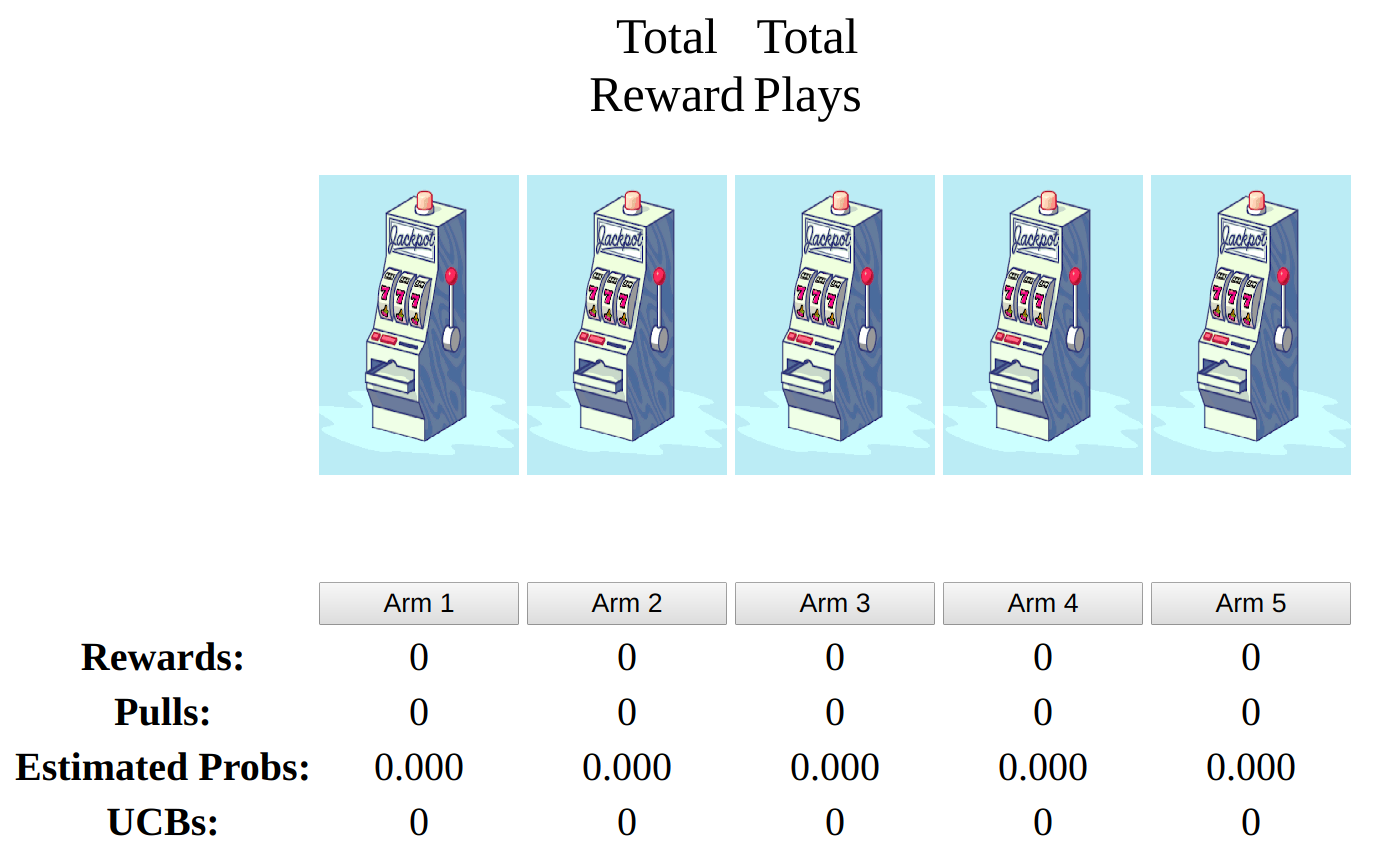
\includegraphics[width=0.75\linewidth]{2-Chapters/2-Chapter/Images/example_of_a_5_arm_bandit_problem__step0.png}
%     \caption{See }
%     \label{fig:2:example_of_a_5_arm_bandit_problem__step0}
% \end{figure}

\begin{figure}[h!]  % [htbp]
    \centering
    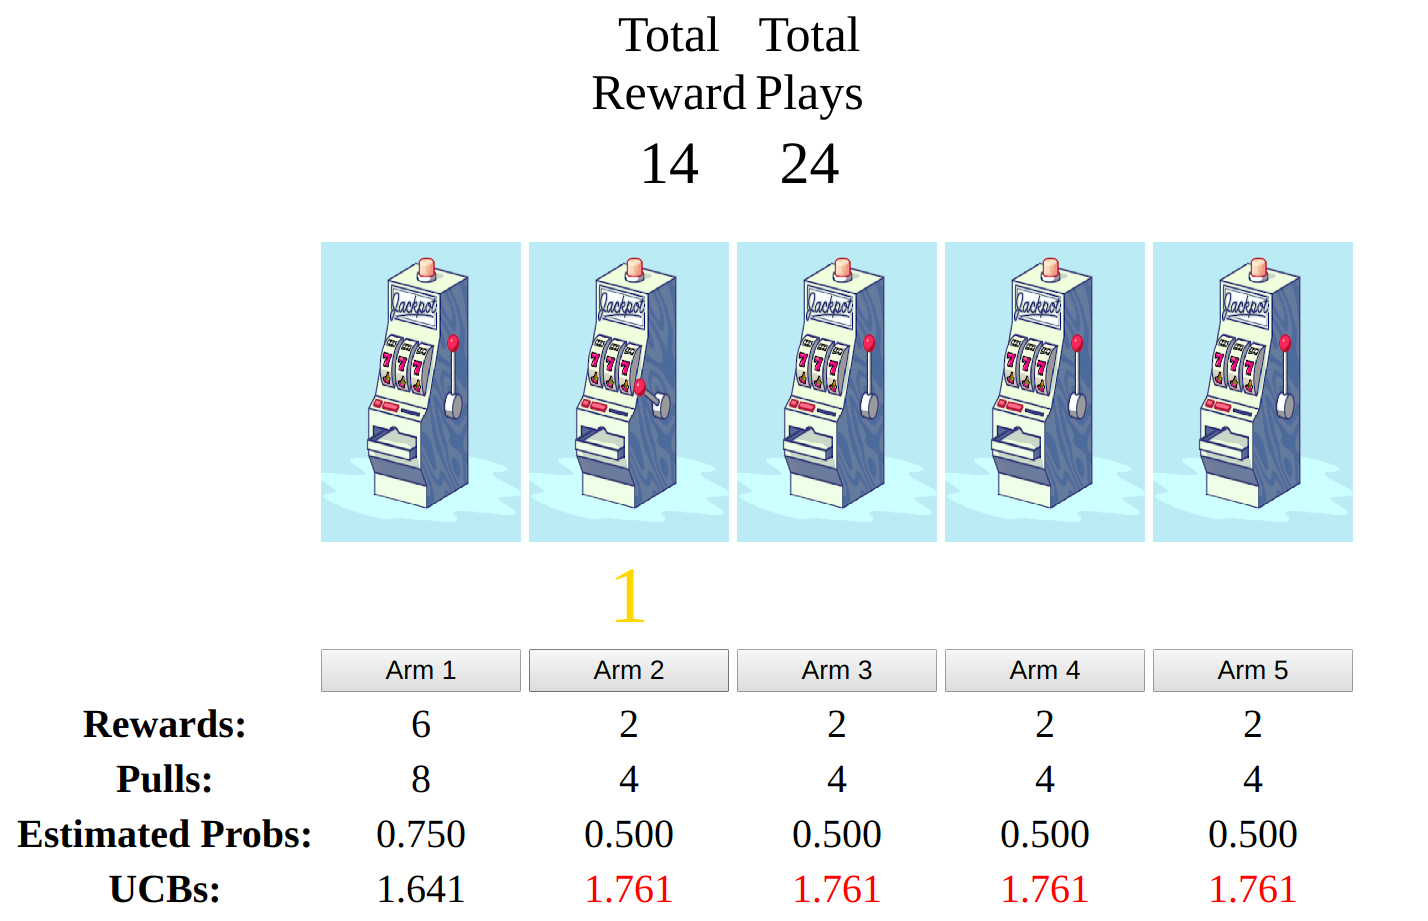
\includegraphics[width=0.85\linewidth]{2-Chapters/2-Chapter/Images/example_of_a_5_arm_bandit_problem.png}
    \caption[Screenshot of the demonstration for a current step of $t=24$.]{Screenshot of the demonstration available online on my website, for a current step of $t=24$.}
    \label{fig:2:example_of_a_5_arm_bandit_problem}
\end{figure}


The webpage looks like Figure~\ref{fig:2:example_of_a_5_arm_bandit_problem} below.
The arms follow Bernoulli distributions, \ie, $\nu_k = \mathcal{B}(\mu_k)$, of unknown means $\mu_k\in[0,1]$, and your goal in this interactive demonstration is to obtain the highest possible cumulated reward in $T=100$ steps, \ie, to maximize $\sum_{t=1}^{100} r(t)$.
Your decisions are made sequentially: at time $t$, you pick one of the arms, $A(t) \in\{1,2,3,4,5\}$, then the demo shows the random reward obtained from this (virtual) casino machine (in \textcolor{gold}{yellow}), \ie, the binary value $r(t)\in\{0,1\}$, that is sampled \iid{} from $\nu_k$.
%
The UI of the demo also shows the current value of $t$ (``total plays'') and $\sum_{s=1}^t r(s)$ the ``total reward''.
For each arm, we show the sum of rewards obtained from that arm, \ie, $X_k(t) \eqdef \sum_{s=1}^t r(s) \mathbbm{1}(A(s) = k)$, in the ``Rewards'' line, and the number of pulls of that arm, \ie, $N_k(t) \eqdef \sum_{s=1}^t \mathbbm{1}(A(s) = k)$ in the ``Pulls'' line.
%
The demo also shows the estimated probability of each arm, that is $\widehat{\mu_k}(t) \eqdef X_k(t) / N_k(t)$ (when $N_k(t)>0$), in the ``Estimated Probs'' line.

In the first Figure~\ref{fig:2:example_of_a_5_arm_bandit_problem}, the current state of the game is shown at time $t=24$.
% Currently at time $t=24$ (out of $T=100$ total time steps),
At this step, the player has collected a sum of rewards of $14$, by observing $X(t) = [6,2,2,2,2]$ rewards of value $1$ in the $K=5$ different arms. Arms were sampled $N(t) = [8,4,4,4,4]$ times, meaning that the value $0$ was seen respectively $[2,2,2,2,2]$ times, and currently arm $1$ appears to be the best one. The true means of the arms are $\bm{\mu}=[0.6, 0.2, 0.55, 0.7, 0.5]$, and (much) more samples are needed before the player can accurately identify arm $4$ as the best arm.
%
In the second Figure~\ref{fig:2:example_of_a_5_arm_bandit_problem__step100} below, we display the result of an example of run, when the player was following the $\UCB_1$ algorithm from \cite{Auer02} (we present it below in Section~\ref{sub:2:IndexPolicies}).
After $T=100$ steps, the player obtained a cumulated reward of $56$, by playing mostly arms $4,3,5,1,0$ (in decreasing order of number of plays). The empirical means $\widehat{\mu_k}(T)$ correctly identify the best arm (arm $4$), but do not correctly rank the arms as arms $1$ and $3$ obtained means of $\widehat{\mu_1}(T) = 0.5 < \widehat{\mu_3}(T)=0.6$ but the true means are $\mu_3 = 0.55 < \mu_1 = 0.6$.
Other examples of such results, for different algorithms, and $T=100$ or $T=10000$, are given in Section~\ref{sub:2:shortNumericalExperiments}.

\begin{figure}[h!]  % [htbp]
    \centering
    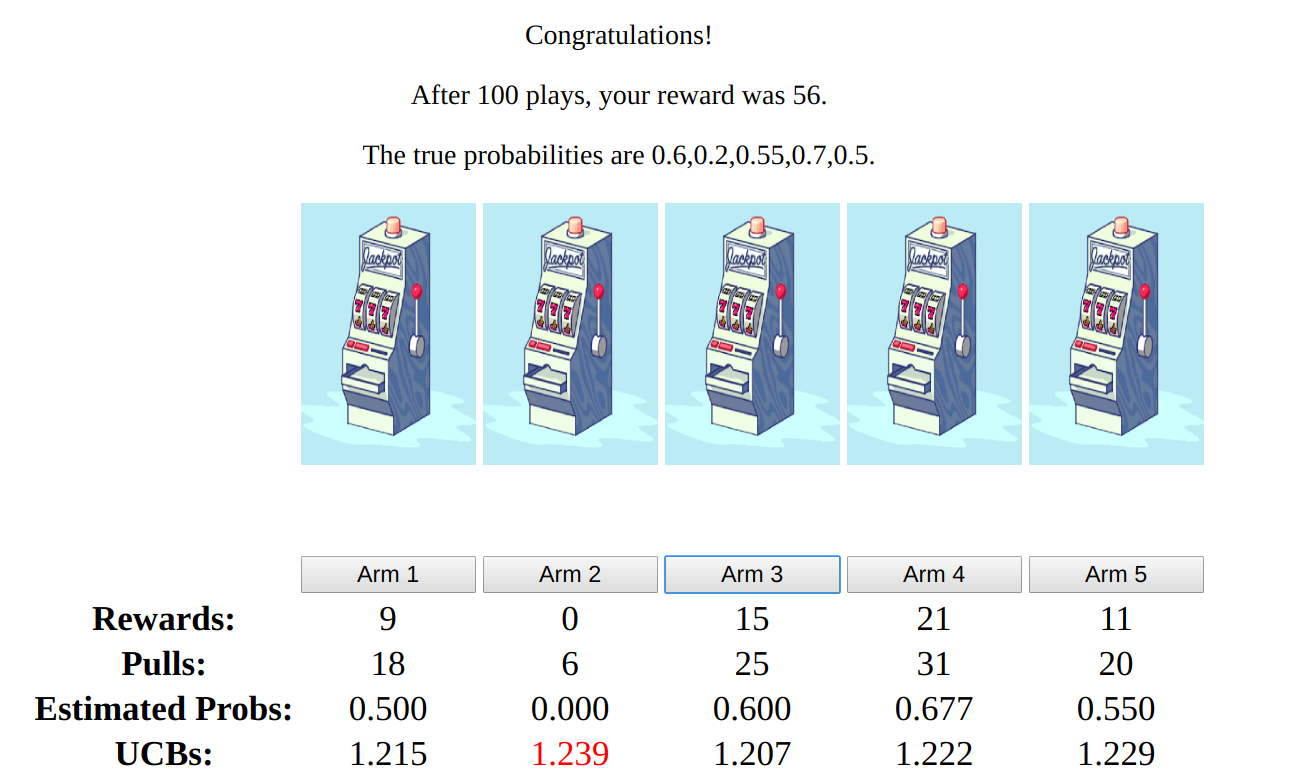
\includegraphics[width=0.85\linewidth]{2-Chapters/2-Chapter/Images/example_of_a_5_arm_bandit_problem__step100.png}
    \caption[Screenshot of the demonstration, at the end of the game after $T=100$ steps]{Screenshot of the demonstration, at the end of the game after $T=100$ steps, where the player suffers from an empirical regret of $R^{\UCB_1}_T = \mu^* T - 56 = 0.7 T - 56 = 14$ after following the $\UCB_1$ algorithm.
        You can try it on \href{https://perso.crans.org/besson/phd/MAB\_interactive\_demo/}{\texttt{perso.crans.org/besson/phd/MAB\_interactive\_demo/}}}
    \label{fig:2:example_of_a_5_arm_bandit_problem__step100}
\end{figure}


\paragraph{Decisions can (and should) depend on the past observations.}

A \emph{bandit algorithm} $\cA$ is also referred to as a strategy or a policy.
% and sometimes it is denoted by $\pi$ or $\rho$ in the literature.
The algorithm $\cA$ selects an arm $A(t)$ at time $t$, possibly by using the past observations and the past external randomness.
As shown below, being oblivious to the past yields very poor performance (cf. the pure exploration policy in Section~\ref{sub:2:naiveSimpleStrategies}), so efficient policies indeed depend on the successive feedbacks.
%
More formally, an algorithm can be defined as a sequence of \emph{measurable} functions $(\cA_t)_{t\geq1}$,
where $\cA_t$ maps the past observations $O_t \eqdef (U_0, Y_{A(1),1}, U_1, \dots, Y_{A(t-1),t-1}, U_{t-1})$
to an arm $\cA_t(O_t) \eqdef A(t) \in[K]$
(we remind that we denote $r(s) = Y_{A(s),s}$ the $s$-th reward).
The initial information is reduced to $O_1 = (U_0)$, and the first decision is $A(1) = \cA_1(O_1)$. Usually, most algorithms starts by selecting $A(1)=1,\dots,A(K)=K$ (or a permutation of the $K$ arms) in the $K$ first steps $t=1,\dots,K$ (\eg, Algorithm~\ref{algo:2:indexPolicy}).
% as illustrated for example in Algorithm~\ref{algo:2:indexPolicy} below.
%
An algorithm is said to be \emph{deterministic} if it does not depend on the external randomness $U_0,U_1,\dots$, but in this thesis \textbf{we only use non-deterministic algorithms}
(in particular, index policies need $U_t$ to break ties in the $\argmax$, see Algorithm~\ref{algo:2:indexPolicy} below).


% ----------------------------------------------------------------------------
\subsection{Common assumptions on the reward distributions}

In the example above, we consider Bernoulli distributions, but other real-valued distributions have been studied in the literature.
From now on and until the last chapter of this thesis, \textbf{we only consider stochastic rewards}. The piece-wise stationary model is studied in Chapter~\ref{chapter:6}.
%
% Everything is implemented and documented at
% https://smpybandits.github.io/docs/Arms.html
\textbf{We also focus only on real-valued rewards}, meaning that $Y_{k,t}\in\R$ for all arm $k$ and time $t$.

An important hypothesis is whether rewards are bounded or not,
and whether the player knows if they are bounded or not before starting the bandit game.
Moreover, if rewards are known to be bounded, let say in an interval $[a,b]$, another important hypothesis is whether the player knows the values of $a$ and $b$ or not.
%
Intuitively, the bandit game is easier if the player knows the support of the distributions, and we restrict to this case in all the thesis, \ie, \emph{$a,b$ are always supposed to be known}.
Most of the algorithms proposed in the literature follow this hypothesis as well.
%
The mostly used
infinitely supported distributions are Gaussian, exponential and Poisson,
while in the literature, the Bernoulli distribution is the most common case of finitely supported distributions.
Continuous-valued distributions with finite support also included truncated versions of infinitely supported distributions, in particular \emph{truncated} Gaussian are used for numerical experiments in lots of research articles.

% Just bounded, in $[a,b]$ but without loss of generality in $[0,1]$ etc.
\paragraph{The normalization trick.}
\label{par:2:normalizationTrick}
%
If the player knows that reward are bounded in an interval $[a,b]$, and if she knows $a$ and $b$ (for $a<b$), then with no loss of generality we can restrict to the interval $[0,1]$, as if $r\in[a,b]$, the player can instead consider the normalized reward $r' = \frac{r-a}{b-a}$ that lies in $[0,1]$.
Note that this ``normalization trick'' is implemented for any policy in our library SMPyBandits, with the \texttt{lower} and \texttt{amplitude} optional arguments, respectively representing $a$ the lower-bound on rewards and $b-a$ the length of the interval of possible values of rewards.

% Bernoulli, Gaussian, sub-Bernoulli, sub-Gaussian, Exponential, sub-Exponential...

% \paragraph{We restrict to one-dimensional exponential family.}
%
% On one-dimensional exponential family...

In the literature, parametric assumptions on the rewards are sometimes considered, typically the assumption that rewards belong to a real-valued distribution lying in an exponential families.
%  or bounded distributions.
One-dimensional exponential families include Bernoulli and Poisson distributions, as well as Gaussian distributions with a fixed variance.
Our main interest is Bernoulli distributions, but we prefer to present the more general notations of exponential families in one dimension.
% We follow the notations from the course on statistical learning (Stat 260) taught in 2010 by Michael Jordan at the University of Berkeley \cite{JordanCourseStatBerkeley}, that are also the notations used for instance in Emilie Kaufmann's PhD in 2014 \cite{Kaufmann12PhD}.

Given a measure $\lambda$, that is usually the natural Lebesgue measure on $\R$, an exponential family of probability distributions is defined as the distributions whose density (relative to $\lambda$) can be written as
% \begin{equation}\label{eq:2:exponentialFamily}
$ \Pr(x | \lambda) = h(x) \exp \left( \eta x - A(\eta) \right)$,
% \end{equation}
for a parameter vector $\eta$ (the canonical parameter), and a sufficient statistic that we restrict to be $T(x)=x$, and a function $h$.
The cumulant function $A(\eta)$ is entirely determined by the $\eta$ and $h$,
as $A(\eta) = \log \left( \int h(x) \exp(\eta x) \lambda(\mathrm{d} x) \right)$.
%
The natural parameter space is the set of values of $\eta$ such that this integral $A(\eta)$ is finite,
and usually the literature focusses on regular and minimal exponential families (when the natural parameter space is an non-empty open set in $\R$).

We have to quote two important results on exponential families:

\begin{enumerate}
    \item
    \emph{A distribution in such family is entirely characterized by its parameter $\eta$}.
    That is why one-dimensional distributions are entirely characterized by their mean, as $\mu = \E_{\eta}[X]$.

    \item
    A second important result is a simplified form for the \emph{Kullback-Leibler divergence} \cite{KullbackLeibler51}, for two distributions lying in the same exponential family.
    The KL divergence is also called the relative entropy is a measure of how one probability distribution is different from a second, reference probability distribution.
\end{enumerate}

\begin{definition}\label{def:2:KLDivergence}
\begin{leftbar}[defnbar]  % XXX leftbar defnbar, comment if needed
    The \emph{Kullback-Leibler divergence} between distributions $d_1$ and $d_2$ is defined as
    \begin{align}\label{eq:2:Kullback-LeiblerDivergenceExpFamily1}
        \KL\left(d_1, d_2\right) \eqdef \int d_1 \log\left(\frac{d_2}{d_1}\right) \lambda(\mathrm{d}x) = \E_{d_1} \left[ \log\left(\frac{d_2}{d_1}\right) \right] \in \mathbb{R}\cup\{\pm\infty\}.
    \end{align}
% \vspace*{-5cm}  % FIXME vspace negative to compensate the \end{leftbar}
\end{leftbar}  % XXX leftbar defnbar, comment if needed
\end{definition}

Following this Definition~\ref{def:2:KLDivergence} for two distributions
$d_1=\Pr(x|\eta_1)$ and $d_2=\Pr(x|\eta_2)$,
we can use a shorter notation and write $\KL( \eta_1, \eta_2 ) \eqdef \KL(\Pr(x|\eta_1), \Pr(x|\eta_2))$, which can be simplified to use only the two parameters $\eta_1$ and $\eta_2$ of $d_1$ and $d_2$,
and $\mu_1 = \E_{\eta_1}[X]$ the mean of distribution $d_1$,
%
% \begin{equation}\label{eq:2:Kullback-LeiblerDivergenceExpFamily2}
$\KL\left( \eta_1, \eta_2 \right) = \E_{d_1}[ (\eta_1 - \eta_2) X ] - A(\eta_1) + A(\eta_2) = (\eta_1 - \eta_2) \mu_1 - A(\eta_1) + A(\eta_2)$.
% \end{equation}
%
Without diving more in the details of exponential families,
it is interesting to illustrate this definition and the notations with two important examples:

\label{par:2:notationsExponentialFamiliesBernoulliGaussian}
\begin{itemize}
    \item
    % $\bullet$
    \textbf{Bernoulli distributions} can be seen as an exponential family with $h(x) = 1$,
    and for a Bernoulli distribution of mean $\mu\in[0,1]$, denoted $B(\mu)$,
    the parameter is $\eta = \mu / (1 - \mu)$, giving $A(\eta) = \log(1 + \mathrm{e}^{\eta})$
    (with the limit behavior $\eta=+\infty$ if $\mu=0$).

    The KL divergence between $B(x)$ and $B(y)$, of parameters $\eta$, $\eta'$ is given by
    $\kl(x,y) \eqdef \KL_{B}(\eta,\eta') = x \log(x/y) + (1-x) \log((1-x)/(1-y))$,
    and it is also called the \emph{relative binary entropy}.
    It satisfies $\kl(x,y) \geq d_{1/4}(x,y)$ (Pinsker's inequality).

    \item
    % $\bullet$
    \textbf{Gaussian distributions} of a fixed variance are a one-dimensional exponential family,
    and in this thesis we do not consider Gaussian with an unknown variance.
    For a variance of $\sigma^2$, the family uses
    % $T(x) = [x ; x^2]^T$ and
    $h(x) = 1/\sqrt{2\pi\sigma^2} \exp(-x^2/(2\sigma^2))$,
    and for a Gaussian distribution with mean $\mu\in\R$, denoted $\cN(\mu,\sigma^2)$,
    the parameter is $\eta = \mu/\sigma^2$, giving $A(\eta) = \mu^2/(2\sigma^2)$.
    % % For a generic variance,
    % This shows that the Gaussian distributions
    % % are a two-dimensional exponential families,
    % with a fixed variance $\sigma^2$ form indeed a one-dimensional exponential family.

    The KL divergence between $\cN(x,\sigma^2)$ and $\cN(x,\sigma^2)$, of parameters $\eta$, $\eta'$ is given by
    $d_{\sigma^2}(x,y) \eqdef \KL_{\cN,\sigma^2}(\eta,\eta') = (x-y)^2 / (2\sigma^2)$
    (see Chapter~8 of \cite{JordanCourseStatBerkeley}).
\end{itemize}


\paragraph{Hypotheses in this thesis.}
%
In the rest of this thesis, \textbf{we only consider bounded rewards in the mathematical developments}, and we mostly focus on Bernoulli distributions, because they are usually the most relevant choice for the considered applications.
First, we restrict for simplicity to Bernoulli distributions for the simulations shown in Chapter~\ref{chapter:3}, even if our library does implement all the distributions commonly found in the literature (including unbounded one-dimensional exponential families and even Markov models).
In Chapter~\ref{chapter:4}, we only study models with binary rewards.
%
Then, when we study multi-players bandits in Chapter~\ref{chapter:5}, we explain that restricting to the Bernoulli case is interesting and not restrictive, as it is actually the hardest case (since continuous distributions has a null mass on $Y_{k,t}=0$, they yield a much simpler problem as the sensing/no sensing distinction no longer makes sense).
%
Finally, in Chapter~\ref{chapter:6} we analyze our proposed algorithm for bounded distributions, without restricting to Bernoulli distributions, but we use the fact that bounded distributions on $[0,1]$ are sub-Bernoulli, and we use the Bernoulli Kullback-Leibler divergence $\kl$ in our analysis.


\paragraph{Other kind of hypothesis: sub-Gaussian and sub-Bernoulli distributions.}
%
A lot of research works considers rewards distributions that are not Gaussian but sub-Gaussian, of a known variance, for instance $1/4$.
For instance, bounded distributions on $[0,1]$ are known to be $1/4$ sub-Gaussian, and this fact is used for instance in \cite{Maillard2018GLR}.
It means that their moment generating function is dominated by that of a Gaussian distribution with the same mean and a variance $1/4$.
In Chapter~\ref{chapter:6}, we instead consider sub-Bernoulli distributions, formally introduced in Definition~\ref{def:6:subBernoulliDistributions}.
%
Such hypothesis is also proposed for other families of distributions, for instance the recent article \cite{KimTewari2019} analyses their Follow-the-Perturbed-Leader algorithm for perturbations following any sub-Weibull distribution (sub-Weibull distributions generalize both sub-Gaussian and sub-Exponential distributions).



\paragraph{About Markov models.}
%
% Markov models: we do not present it in this thesis.
Finally, we note that Markov models, while being implemented in SMPyBandits, are not used in this thesis.
They were introduced in the 1980s, by Whittle in \cite{Whittle1988} and Anantharam and others in \cite{Anantharam87b}.
A Markov MAB model maps an arm to a Markov chain \cite{Norris98}, instead of a distribution, and thus they are no longer stochastic nor stationary.
Such Markov models come in two flavors: rested or restless.
For $K$ arms, each Markov chain has a finite number of states $s$, each corresponding to a (constant) reward that the player obtains if she selects this arm while its Markov chain is in state $s$.
Rested Markov models means that only the state of the selected arm's Markov chain can change, following its Markov transition matrix.
Restless models remove this hypothesis, making them harder to track and solve.
%
Such models were less studied than stationary or adversarial models, but some interesting works focused on Markov models in the last 10 years\footnote{~
For instance, \cite{Melian15} proposed a cognitive radio model mixing MAB and Hidden Markov Models (HMM), solved by a mixed policy called UCB-HMM.}.
A curious reader about Markov chains could start to read Chapter~3 of \cite{LattimoreBanditAlgorithmsBook} (Section~3.2) and then refer to the famous book \cite{Norris98}.


% ----------------------------------------------------------------------------
\section{Different applications of stochastic MAB}
\label{sec:2:applicationsofStochasticMAB}

The blooming success of the research on multi-armed bandits is easily explained by the different spectrum of applications of MAB models to real-world discrete-time decision making problems.
This research field has been very active since the years 2010s, but it started as early as 1933 with \cite{Thompson33}, and was active since the 1980s and the seminal works by Lai and Robbins \cite{LaiRobbins85} and by Anantharam and others \cite{Anantharam87a}.
%
MAB have been applied successfully to various decision making problems, like the following:

\textbf{Clinical trials} have been the first historical application of MAB models, where an arm represents a treatment, and the distribution associated with such treatment can be a Bernoulli distribution: a reward of $0$ means the drug did not heal the disease, and a reward of $1$ indicates a success. The mean of an arm, in this application, represents the mean success rate of a treatment, and the goal of a doctor in a clinical trial is to identify the best treatment, \ie, the arm with highest mean, in a number of trials as short as possible.
%
% After introducing formally the notations used in all this thesis, we review below possible applications of multi-armed bandits.

% Other popular applications include the following.
%
% \begin{itemize}
%     \item
    \textbf{A/B testing}, for instance for websites, is a popular application of the best arm identification problem,
    where the task is purely exploratory and the player is asked to identify the best of two options (or more), in a finite number of steps \cite{audibert2010best}.
    The problem can either consider a fixed budget and no freedom on the ending of the game (\ie, an known horizon $T$), or a fixed confidence and a certain freedom on the budget (\ie, the identified arm must be the true best arm with probability at least $1-\delta$) \cite{Garivier16BAI}.
    The theoretical complexity of this problem
    % use of bandit for A/B testing
    was first studied in \cite{Kaufmann14},
    and a more practical point-of-view was proposed in \cite{Jamieson17ABTest}.

    % \item
    MAB can also be applied to a broader setting of \textbf{online content recommandation},
    with more than two options.
    The seminal work of \cite{Li10} studies the application of contextual bandit to news article recommendation, as it is used in practice on platforms such as Microsoft's Bing news website,
    or in applications like Netflix.
    In such models, the arms correspond to items to recommend (\eg, articles or movies), and the contexts contain features about each user of the system.
    An interesting work is \cite{Louedec16}, who studies slowly-varying non-stationary models applied to recommender systems.

    % \item
    Using bandit algorithms for \textbf{improved machine learning} models or algorithms has been an active research domain for the last ten years or so.
    As presented below in Section~\ref{sec:2:chooseYourPreferredBanditAlgorithm}, a certain ``leader'' bandit algorithm can be used to select on the run the best bandit algorithm from a pool of ``followers'' algorithms.
    Other possible use cases include hyper-parameter optimization, or features selection.
    Hyper-parameters include real-valued parameters, like $\alpha\in[\frac{1}{2},\infty)$ for the $\UCB_1$ or $\varepsilon\in(0,1)$ for the $\varepsilon$-greedy bandit algorithms, a step size multiplier in a gradient method, or the width of a radial based function (RBF) kernel method.
    Discrete-valued parameters are also common, like a choice in a fixed set of kernel functions or the depth of neural networks,
    and higher dimensional or more complex hyper-parameters can for instance be the entire architecture of a neural network.

The different applications detailed above are still active research directions,
and a curious reader can find other interesting applications of MAB models and algorithms in \cite{bouneffouf2019survey}, such as game tree search or network routing in Section~1.2 of \cite{LattimoreBanditAlgorithmsBook}.


\textbf{Applications for Opportunistic Spectrum Access.}
% Detail the previous work from our team SCEE on bandits + OSA : Wassim, Navik
%
As highlighted in Chapter~\ref{chapter:1},
the focus of this work is on cognitive radio and IoT networks, where arms can represent wireless orthogonal channels, but more generally any resource characterizing the communication between a wireless device and a gateway (\eg, spreading factor for LoRa \cite{KerkoucheAlami18}, power allocation for NOMA etc).
% In cognitive radio using centralized supervision, for instance if the gateway can decide the allocation of devices to resources, MAB can also be used to let the gateway explore different allocations and learn by itself a good allocation, see for instance this article that consider 5G-like networks with small cells \cite{Maghsudi16}.
%
% Previous works of our SCEE team showed that MAB can be used to model the problem of spectrum access for a secondary user accessing a licensed spectrum.
% In this model, arms represent a finite set of orthogonal channels, \ie, different frequency bands in a licensed spectrum.
In the model of Opportunistic Spectrum Access (OSA) with sensing, the samples $Y_{k,t}$ represents the feedback obtained by the CR-equipped device after sensing the channel $k$ at time $t$.
A reward of $r(t) = 1$ indicates that no Primary User was sensed, while a reward of $r(t)=0$ indicates that the channel $k$ is busy at time $t$ and no uplink message can be sent.
%
This model was first introduced by Wassim Jouini during his PhD thesis,
in \cite{Jouini09} and later studied in both \cite{Jouini10,Jouini12}.
Proof-of-concepts using real-world radio hardware was first proposed in \cite{MoyWSR2014,RobertSDR2014}.
%
We study a similar model of using MAB for Cognitive Radio but without the OSA strucutre of Primary and Secondary users, \ie, without sensing information but only a collision indicator, in Chapters~\ref{chapter:4} and \ref{chapter:5}.


% ----------------------------------------------------------------------------
\section{Definition, decomposition and lower-bounds on the regret}
% : definition, decomposition, and lower bounds
\label{sec:2:lowerUpperBoundsRegret}

As explained above, the main objective of a player facing a bandit game is to maximize its (expected) cumulated reward.
An efficient algorithm should see its mean reward converge to the maximum reward.
We introduce in this section the notion of \emph{regret}, and the equivalence for a player between maximizing its sum of rewards and minimizing its regret.
In Machine Learning, we usually prefer to aim at minimizing certain quantities, such as the error rate in supervised learning, or the distance to the optimum in an optimization problem,
but the main interest of studying the regret is to be able to obtain higher-order information about the convergence of the mean reward to the max reward,
or in other words, to quantify the speed of convergence of a MAB algorithm.


\subsection{Measuring performance with the (mean) regret}

Let us first introduce some notations.
We consider a stochastic and stationary MAB problem, with $K$ arms of distributions $\nu_1,\dots,\nu_K=(\nu_k)_k$, that generates \iid{} samples $Y_{k,t} \sim \nu_k$, for any time $t$.
% with $r(t)=Y_{A(t),t}$).
We focus on distributions fully characterized by their means, that can be Bernoulli or any one-dimensional exponential family.
We denote $\mu_k \eqdef \E[Y_{k,t}] \in \R$ the mean of the distribution of arm $k$ (it will be referred to as the \emph{mean of arm $k$}).
%
% \paragraph{Defining the regret.}
%
To define the regret, we first need to distinguish between \emph{optimal} and \emph{sub-optimal} arms.

\begin{definition}\label{def:2:optimalSubOptimalArms}
\begin{leftbar}[defnbar]  % XXX leftbar defnbar, comment if needed
    % [Optimal and sub-optimal arms]
    Consider a bandit problem of $K$ arms with distributions of means $\bm{\mu}=\mu_1,\dots,\mu_k$.
    Denote $\mu^* \eqdef \max_k \mu_k$ the largest mean.
    The best arm can be non unique, and any arm $k$ having $\mu_k = \mu^*$ is said to be \emph{optimal},
    while arms satisfying $\mu_k < \mu^*$ are called \emph{sub-optimal}.
\end{leftbar}  % XXX leftbar defnbar, comment if needed
\end{definition}

If the goal of the player is to maximize $\E\left[\sum_{t=1}^T r(t)\right]$,
the optimal strategy for this bandit problem is to always pull one of the optimal arms (it can be not unique), but it is unrealistic as the player does not know the true means, nor the optimal arms (as long as they are not all optimal, \ie, in non trivial problems).
%
Comparing the difference between the performance of a fixed baseline and that of the player is a common approach in machine learning research,
and here we can compare with the oracle strategy that always obtains an (expected) reward of $\mu^*$.
%
For a fixed horizon $T$, if $k^*$ denotes the index of any optimal arm,
let us introduce the (mean) regret $R_T^{\cA}$ of an algorithm $\cA$ as
$R_T^{\cA} \eqdef \E\left[ \sum_{t=1}^T (Y_{k^*,t} - r(t)) \right]$.
%
As the rewards from arm $k^*$ are \iid{} (as for all arms), and by linearity of the expectation, we can rewrite this expression to obtain the following definition of the regret:
\begin{align*}
    R_T^{\cA}
    & = \E\left[ \sum_{t=1}^T (Y_{k^*,t} - r(t)) \right]
    = \E\left[ \sum_{t=1}^T \underbrace{Y_{k^*,t}}_{\text{\iid{} from $\nu_{k^*}$}} \right] - \E\left[ \sum_{t=1}^T r(t) \right] \\
    & = T \times \E\left[ Y_{k^*,1} \right] - \sum_{t=1}^T \E\left[ r(t) \right]
    = T \mu^* - \sum_{t=1}^T \E\left[ r(t) \right].
\end{align*}
% This is the definition we give below.


\begin{definition}[Regret]\label{def:2:regret}
\begin{leftbar}[defnbar]  % XXX leftbar defnbar, comment if needed
    For an algorithm $\cA$, a bandit problem of $K$ arms characterized by their means $\mu_1,\dots,\mu_K$, with $\mu^* \eqdef \max_k \mu_k$, then its \emph{(mean) regret} at horizon $T$ is $R_T^{\cA}$ defined as
    %
    \begin{align}\label{eq:2:regret}
        R_T^{\cA}
        \eqdef \E\left[ \sum_{t=1}^T (Y_{k^*,t} - r(t)) \right]
        % = T \mu^* - \sum_{t=1}^T \E\left[ Y(t) \right]
        = T \mu^* - \sum_{t=1}^T \E\left[ r(t) \right].
    \end{align}
% \vspace*{-20pt}  % FIXME vspace negative to compensate the \end{leftbar}
\end{leftbar}  % XXX leftbar defnbar, comment if needed
\end{definition}

One first need to observe that $R_T^{\cA} \geq 0$ for any $T$ and $\cA$, and that $R_T^{\cA} \leq \mu^* T$ (if rewards lie in $[0,1]$).
Thus any algorithm has $R_T^{\cA} = \bigO{T}$, which justifies why we are interested in efficient algorithms that achieve at least a sub-linear regret, \ie, $R_T^{\cA} = \smallO{T}$.

\paragraph{A useful decomposition of the regret.}
%
Remember that $N_k(t) \eqdef \sum_{s=1}^t \mathbbm{1}(A(s) = k)$ denotes the number of times arm $k$ was selected between times $1$ and $t$,
%
and that the samples $Y_{k,t}$ are all \iid{} of mean $\mu_k$.
The \emph{gap} between any arm $k\in[K]$ and an optimal arm is defined as $\Delta_k \eqdef \mu^* - \mu_k$
(an arm $k$ is thus sub-optimal if and only if $\Delta_k > 0$),
and thus we can write the following decomposition on the regret.

\begin{lemma}[Regret decomposition]\label{lem:2:RegretDecomposition}
\begin{leftbar}[lemmabar]  % XXX leftbar lemmabar, comment if needed
    The (mean) regret $R_T^{\cA}$ can be decomposed as a sum of the number of selections of sub-optimal arms $k$, weighted by their gaps:
    \begin{align}\label{eq:2:RegretDecomposition}
        R_T^{\cA} = \sum_{k=1}^K \Delta_k \; \E[ N_k(T) ]
        = \sum_{\substack{k=1,\dots,K\\\Delta_k > 0}} \Delta_k \; \E[ N_k(T) ].
    \end{align}
    % \vspace*{-20pt}  % FIXME vspace negative to compensate the \end{leftbar}
\end{leftbar}  % XXX leftbar lemmabar, comment if needed
\end{lemma}
%
\begin{smallproof}\label{proof:2:RegretDecomposition}
    We use the chain rule of expectation and a conditioning on $O_t$,
    because the expectation is taken on the randomness of the (\iid) samples $(Y_{k,t})_t$ and on the decisions of the player $(A(t))_t$, which are measurable wrt to the past observations $O_t = (U_0, Y_{A(1),1}, U_1, \dots, Y_{A(t-1),t-1}, U_{t-1})$.
    Thus we can rewrite the expected cumulated reward as follows:
    %
    % FIXME add a blank line or a negative space if it looks weird
    %
    % \vspace*{-20pt}
    \begin{align*}
        \E \left[ \sum_{t=1}^T r(t) \right]
        &= \E \left[ \sum_{t=1}^T \sum_{k=1}^K Y_{k,t} \mathbbm{1}(A(t) = k) \right]
        = \sum_{k=1}^K \sum_{t=1}^T \E \left[ Y_{k,t} \mathbbm{1}(A(t) = k) \right] \\
        &= \sum_{k=1}^K \sum_{t=1}^T \E \Bigl[ \E \left[ Y_{k,t} | O_t \right] \mathbbm{1}(A(t) = k) \Bigr]
        = \sum_{k=1}^K \sum_{t=1}^T \E \Bigl[ \E \left[ Y_{k,1} \right] \mathbbm{1}(A(t) = k) \Bigr] \\
        &= \sum_{k=1}^K \underbrace{\E \left[ Y_{k,1} \right]}_{\mu_k} \underbrace{\sum_{t=1}^T \E \left[ \mathbbm{1}(A(t) = k) \right]}_{= N_k(T)}
        % = \sum_{k=1}^K \mu_k \E \left[ \sum_{t=1}^T \mathbbm{1}(A(t) = k) \right]\\
        = \sum_{k=1}^K \mu_k \E \left[ N_k(T) \right].
    \end{align*}
    %
    Thus $R_T^{\cA} = T \mu^* - \sum_{t=1}^T \E\left[ r(t) \right] = T \mu^* - \sum_{k=1}^K \mu_k \E[ N_k(T) ] = \sum_{k=1}^K (\mu^* - \mu_k) \E[ N_k(T) ]$,
    as $\sum_{k=1}^K  \E[ N_k(T) ] = T$.
    The sum can then be simplified to only account for sub-optimal arms, \ie, arms $k$ such that $\Delta_k > 0$.
\end{smallproof}


\paragraph{Consequences.}
%
Such decomposition of the regret can be useful for at least two reasons:

% \begin{itemize}
%     \item
On the one hand, from a numerical simulation point-of-view, when we run a finite number of repetitions of the same stochastic experiment, if we want to compute and visualize the regret, we can either use the definition with the rewards, or the decomposition and simply sum the gaps $\Delta_k$ with the number of sub-optimal draws.
Both quantities are indeed equal \emph{in expectation}, but with only a finite number of trajectories and observations, the first estimate is more noisy than the second one, since the randomness on the rewards is (partially) removed in the decomposition \eqref{eq:2:RegretDecomposition} (thanks to the conditioning on $O_t$ done in the proof).
In our library SMPyBandits, we implement both estimators, and all values of regret used in this thesis are based on the one using the decomposition of Lemma~\ref{lem:2:RegretDecomposition}, because it gives faster convergence, and also ``smoother'' plots.
\label{remark:2:moreAccurateCountofRegretForSimulations}

    % \item
On the other hand, this decomposition is necessary as theoretical analyses of the regret of (single-player) MAB algorithms are usually based on controlling the suboptimal draws $N_k(T)$ and not directly the regret $R_T^{\cA}$.
Even if we prove that controlling $N_k(T)$ is no longer sufficient to obtain low regret for the multi-players case, we extend this decomposition in Chapter~\ref{chapter:3} (in Lemma~\ref{lem:5:DecompositionRegret}), and it is the first quantity we prove to be bounded by $\bigO{\log(T)}$ when we prove the regret upper-bound of our proposal \MCTopM-\klUCB.
% \end{itemize}


\subsection{Regret lower bounds}

We include here two well-known results about what bandit algorithms \emph{cannot} do.
First, a \emph{problem-dependent lower-bound} states that any algorithm suffers a regret at least $\Omega(\log T)$ on any problem (from \cite{LaiRobbins85}).
Then, a \emph{worst-case result} states that any algorithm can perform as badly as $\Omega(\sqrt{K T})$ on a certain problem instance, designed specifically to make it perform badly (a result from \cite{Auer02NonStochastic}),
%
In certain families of problems, \eg, $K$ Bernoulli distributed arms, the difficulty of a problem is characterized by a constant that depends only on the arms means. This measure of difficulty of a problem is hidden in the $\Omega$ notation in these lower-bounds.

In all this section, we restrict to stationary stochastic problems with $K\geq2$ arms.
We do not give proofs of the following theorems, as they can be found in the historical papers, and simpler proofs are given in recent references, such as \cite{Bubeck12}, \cite{LattimoreBanditAlgorithmsBook}, or Chapter~2 in \cite{Slivkins2019} for instance.
%
Let $\cI$ denote the set of all problem instances, with $K \geq 2$ arms. We assume the rewards lie in $[0,1]$ (but no additional hypothesis).
To specify the dependency on an instance $I$, we denote the regret of $\cA$ on instance $I$ and horizon $T$ by $R_T^{\cA}(I)$.


\paragraph{Problem-dependent lower-bound in $\Omega(\log T)$.}
%
The following two theorems were proven in \cite{LaiRobbins85}.
These lower-bounds are of highest interest to design efficient algorithms,
and a significant part of the research literature on MAB algorithms has focused on finding algorithms that matches the Lai and Robbins' lower-bound asymptotically.
This means that an upper-bound is proven on the regret of algorithm $\cA$, that asymptotically matches the lower-bound, with the same constant in the big-$\cO$ notation (in which case we say that the algorithm is \emph{optimal}), or with a larger constant (the algorithm is said to be \emph{order-optimal} in such case).


\begin{theorem}\label{thm:2:firstLogTLowerBound}
\begin{leftbar}[theorembar]  % XXX leftbar theorembar, comment if needed
    \emph{No algorithm $\cA$ can achieve} a (mean) regret $R_T^{\cA}(I) = \smallO{c_I \log(T)}$ for all problem instances $I \in \cI$,
    where this notation means that the ``constant'' $c_I$ can depend on the problem instance $I$ (\eg, on the means and on $K$) but not on the time horizon $T$.
\end{leftbar}  % XXX leftbar theorembar, comment if needed
\end{theorem}

We consider uniformly efficient\footnote{This notion is then extended to ``\emph{strongly uniformly efficient} algorithms'', in the multi-players case with Definition~\ref{def:5:DecentralizedUniformEfficiency}, where we also include a notion of (expected) fairness.} algorithms, to rule out algorithms achieving low regret on some problem instances while achieving linear regret on other instances.
In particular, it is necessary to rule out algorithms that always pick the same arm, as on some problem instances such fixed-arm algorithms can achieve zero regret.

\begin{definition}\label{def:2:uniformlyEfficientAlgorithm}
\begin{leftbar}[defnbar]  % XXX leftbar defnbar, comment if needed
    An algorithm $\cA$ is \emph{uniformly efficient} if its (mean) regret satisfies
    $R_T^{\cA}(I) = \smallO{C_{I,\alpha} T^{\alpha}}$,
    for any value $\alpha>0$ and any problem instance $I\in \cI$,
    where this notation means that the ``constant'' $C_{I,\alpha}$ can depend on the problem instance $I$ and on $\alpha$, but \emph{not} on the time horizon $T$.
\end{leftbar}  % XXX leftbar defnbar, comment if needed
\end{definition}

This family is non-empty as it contains for instance the $\UCB_1$ algorithm, since its regret is proven to be logarithmic on any problem instance with bounded rewards (in Theorem~\ref{thm:2:UCBregretBound} below).
Now we can state the second logarithmic lower-bound, for algorithms in this family:

\begin{theorem}\label{thm:2:secondLogTLowerBound}
\begin{leftbar}[theorembar]  % XXX leftbar theorembar, comment if needed
    If $\cA$ is uniformly efficient,
    then for any arbitrary problem instance $I$,
    there exists a constant $C_I$ depending only on $I$,
    and a time $T_0$ such that $\forall T \geq T_0, \;\;\; R_T^{\cA}(I) \geq C_I \log(T)$.
\end{leftbar}  % XXX leftbar theorembar, comment if needed
\end{theorem}

This third theorem specifies possible values of the constants $C_I$ for the two previous results.

\begin{theorem}\label{thm:2:forSecondLogTLowerBound}
\begin{leftbarnospace}[theorembar]  % XXX leftbar theorembar, comment if needed
    Let $\cA$ denote a uniformly efficient algorithm,
    and $I$ an arbitrary problem instance.
    \begin{itemize}
        \item
        The bound from Theorem~\ref{thm:2:secondLogTLowerBound} holds with,
        % \begin{equation}\label{eq:2:forSecondLogTLowerBound}
        $C_I = \mu^* (1 - \mu^*) \sum\limits_{k: \Delta_k > 0} \frac{1}{\Delta_k}$.
        % \end{equation}
        \item
        For any $\varepsilon>0$, the bound from Theorem~\ref{thm:2:secondLogTLowerBound} also holds with,
        % \begin{equation}\label{eq:2:forSecondLogTLowerBound2}
        $C_I = \sum\limits_{k: \Delta_k > 0} \frac{\Delta_k}{\KL(\mu_k, \mu^*)} - \varepsilon$.
        % \end{equation}
    \end{itemize}
\end{leftbarnospace}  % XXX leftbar theorembar, comment if needed
\end{theorem}

Moreover, it is interesting to note that the second lower-bound of Theorem~\ref{thm:2:forSecondLogTLowerBound} can be directly used to design efficient algorithms\footnote{~Tracking this quantity, by using empirical estimates of the means, is used for instance in the OSSB algorithm proposed in \cite{Combes17}, which is proven to attain the lower-bound for a wider range of problems (for problems called structured stochastic bandits).}, as thanks to the regret decomposition given in Lemma~\ref{lem:2:RegretDecomposition} above, the expression of $C_I$ essentially says that any efficient algorithm
should sample each sub-optimal arm $k$ about $\log(T)/\KL(\mu_k,\mu^*)$ times in the total of $T$ time steps.


Many algorithms have been proven to achieve logarithmic regret in the stochastic case,
and in particular it is the case of the algorithms used in this thesis, $\UCB_1$ from \cite{Auer02}, Thompson sampling from \cite{Thompson33} and analyzed in \cite{AgrawalGoyal11,Kaufmann12Thompson}, and \klUCB{} from \cite{Garivier11KL,KLUCBJournal}.
%
Such bounds are valid in different settings, and in particular $\UCB_1$ is order-optimal for bounded rewards or one-dimensional exponential families,
while Thompson sampling is optimal for bounded rewards, and \klUCB{} have been proven to be optimal for both cases.
%
For more details, we refer to Chapter~16 of \cite{LattimoreBanditAlgorithmsBook}.


\paragraph{Worst-case lower-bound in $\Omega(\sqrt{T})$.}
%
For a fixed horizon $T$, it is interesting to note that one can find instances $I$ that are so ``hard'' that a logarithmic regret (lower or upper) bound that uses a constant $C_I$ no longer brings any information.
Indeed, we can naively bound the regret by $R_T^{\cA} \leq (\max_k \Delta_k) T$, and thus if $(\max_k \Delta_k)$ can be taken so small that $C_I \log(T) \gg (\max_k \Delta_k) T$, and thus a regret upper bound like $R_T^{\cA} \leq C_I \log(T)$ is useless.
%
\begin{smallproof}\label{proof:2:worstCaseLowerBound}
    For an example, consider any large horizon $T>10$, and $K=2$ Bernoulli arms.
    Chose any small $\varepsilon$ such that $\varepsilon \ll \sqrt{4 \log(T) / T}$, then chose let $\mu_1 = 1/2$ and $\mu_2 = 1/2 - \varepsilon$.
    The constant $C_I$ from the first case of Theorem~\ref{thm:2:forSecondLogTLowerBound} is $C_I = 1 / (4 \varepsilon)$ and $\Delta=\varepsilon$ and it becomes so large that
    the logarithmic upper-bound is useless in such case, as
    $\varepsilon \ll \sqrt{\frac{4 \log(T)}{T}} \Longleftrightarrow \frac{1}{4\varepsilon} \log(T) \gg \Delta T$.
\end{smallproof}

For this reason, the research literature has also been interested by another family of regret bounds, that are not problem-dependent but worst-case, or also called minimax \cite{Audibert2009minimax,audibert2010minimax} or problem-independent.
Hence it is interesting to quote another lower-bound on the regret, that can bring useful information in such settings.
The following theorem is from \cite{Auer02NonStochastic}.
%
For more details, we refer to Chapter~15 of \cite{LattimoreBanditAlgorithmsBook}.

\begin{theorem}\label{thm:2:worstCaseLowerBound}
\begin{leftbar}[theorembar]  % XXX leftbar theorembar, comment if needed
    Fix the number of arms $K$, and an algorithm $\cA$.
    Then for any horizon $T$, there exists a problem instance $I_T$ on which the algorithm suffers at least a regret $R_T^{\cA}(I_T) \geq \Omega(\sqrt{K T})$.
\end{leftbar}  % XXX leftbar theorembar, comment if needed
\end{theorem}

Similarly to what is considered for the first lower-bound,
a natural question is to know if there is an algorithm that achieve a regret upper-bound of the form $R_T^{\cA}(I) \leq \bigO{\sqrt{K T}}$ for any instance, independently on the problem difficulty.
It is the case for the Exp3 algorithm from \cite{Auer02}, for example.
Since a few years, some algorithms were shown to achieve both a problem-dependent logarithmic and a minimax upper-bounds,
like MOSS in \cite{Audibert2009minimax} or recently \KLUCBpp{} in \cite{Menard17},
and such results are usually referred to as ``best of both worlds''.


% % do not detail too much, don't explain the tools behind the result

% \begin{itemize}
%     \item
%     - [Lai and Robbins] lower-bound in $\Omega(\log(T))$ \cite{LaiRobbins85}
%     \item
%     - Worst case lower-bound in $\Omega(\sqrt{T})$ \cite{Auer02,Auer02NonStochastic,Bubeck12}
%     \item
%     - Adversarial lower-bound in $\Omega(\sqrt{T})$ (also useful for piece-wise stationary models) \cite{Auer02NonStochastic}
% \end{itemize}


\subsection{Other measures of performances}

In this thesis, we only study analytically the mean regret $R_T^{\cA}$ (in Chapters~\ref{chapter:5} and \ref{chapter:6}), but we quickly mention other measures of performances used in our work.

% - Quantile regret or just histogram of regrets
First, when doing numerical experiments about bandits, if one studies the regret as an empirical mean based on a ``large'' number of random repetitions (\eg, $N=1000$ repetitions), it is important to not only show the mean value but also the variance of the values taken by the regret on each repetition, to verify that all algorithms perform consistently.
Indeed, by only visualizing the mean of $1000$ values, it is possible that we miss some ``bad runs'': if $1$ run out of the $1000$ gives linear regret (\ie, $R_T^{\cA} \propto T$) and the $999$ other give logarithmic regret, then the mean will appear logarithmic.
This is the case of the \Selfish{} algorithm that is defined and explored in Chapter~\ref{chapter:5}.
By visualizing the entire \emph{distribution} (as an histogram), or the variance of the values of $R_T^{\cA}$, and if the number $N$ is reasonably large, we can verify that the regret appears logarithmic for all runs.

% DONE on s'en fout !
% % - Best Arm Identification?
% Other measures of performance that has been studied in the literature include
% the best arm identification (BAI) rate
% and the best arm selection (BAS) rate.
% The BAI rate counts the frequency at which an algorithm $\cA$ correctly identified the best arm(s) at the horizon $T$,
% while the BAS rate counts the total number of time steps during which $\cA$ selected (one of) the best arm(s).
% Both quantities are computed and stored in all numerical simulations using SMPyBandits, but visualizations for both have not been included in this thesis.

% - Worst case regret (max $R_T^{r}$ for $r$ index of Monte-Carlo simulation?)
The \textbf{switching cost} $\mathrm{SC}^{\cA}(T)$ counts how many times the player's decision has changed from one time step to the next one, \ie, $\mathrm{SC}^{\cA}(T) \eqdef \sum_{t=1}^{T-1} \indic(A(t) \neq A(t+1))$.
It has recently gained interest in the literature, for instance the authors of \cite{Koren17} proposed an algorithm that adaptively tries to balance the trade-off between minimizing the regret and minimizing the switching cost.
%
Indeed, in single-player models it is easy to show that achieving logarithmic regret directly implies a logarithmic upper-bound on the switching cost, and conversely the lower-bound from \cite{LaiRobbins85} also gives an asymptotic logarithmic lower-bound.
But even if $\mathrm{SC}^{\cA}(T) = \Theta(\log T)$ for an efficient algorithm, it can be interesting to numerically evaluate this quantity, as a large value might indicate an algorithm that is alternating too much between the optimal arm and other arms.
%
% \TODOL{Enlever ça, juste une phrase qui dit "on le fait plus tard".}
We find more interesting to study $\mathrm{SC}^{\cA_1,\dots,\cA_M}(T)$, the sum of the switching costs of the $M$ players in a multi-players bandit game (if player $j$ uses algorithm $\cA_j$ for $j=1,\dots,M$), as studied in Chapter~\ref{chapter:5}.
% Indeed in this case it is possible that the players attain a logarithmic centralized regret, by following an efficient centralized or decentralized algorithm, while still suffering from a linear switching cost.
% %
% It is very satisfying to obtain a logarithmic switching cost for our algorithm \MCTopM-\klUCB{} in Chapter~\ref{chapter:5}, even if minimizing the switching cost was not one of our objective, and the bound we obtain on $\mathrm{SC}^{\cA_1,\dots,\cA_M}(T)$ is just a consequence of our proof of the control we give on the regret $R^{\cA}(T)$.
% % - Switching cost? \cite{modiDemo2016} \cite{Koren17}
% On a more experimental note, it was shown in \cite{modiDemo2016} that the previous state-of-the-art policy for multi-players bandits, \rhoRand, could be tuned to run in batches\footnote{~The batch bandit setting implies that all players use the same decisions for instance for $50$ consecutive times, and update their decisions only once every $50$ time steps. For more details, see \cite{modiDemo2016} for experiments on the multi-players case, or \cite{perchet2016,gao2019batched,kolnogorov2019multi} for theoretical developments on the single-player case.}, in order to reduce by a certain multiplicative factor its switching cost while only adding an additive factor on its regret. While such ideas can interest a practitioner, they does not change the asymptotic behavior of $\mathrm{SC}^{\cA_1,\dots,\cA_M}(T)$, which is $\Theta(\log(T))$ for any efficient policy.


% - Fairness ?
Finally, another interesting measure of performance is the \textbf{fairness}.
It was not studied much for single-player problems, and usually it means that each arm must be explored at least a given fraction of the total horizon $T$ (\ie, ``arm-wise fairness'').
It was studied in a very recent article \cite{Patil2019stochastic},
where a different notion of regret is introduced to account for the fairness constraint. The authors show that different algorithms, based on $\UCB_1$ or Thompson sampling, can achieve logarithmic regret while respecting the fairness constraints.
%
% \TODOL{Enlever ça, juste une phrase qui dit "on le fait plus tard".}
In this thesis, we only consider fairness in the multi-players bandit models,
in Chapter~\ref{chapter:5}, where fairness refers to a different notion (\ie, ``cooperative fairness'').
% When $M<K$ players learn in a decentralized way, they will essentially converge to an orthogonal affectation of players to arms, so that each player uses a unique arm among the $M$ best arms (most of the times).
% The fairness constraint says that, in average, no user is arbitrarily going to converge more frequently on a better arm than another user, and it is for instance the case for permutation invariant decentralized algorithms.
We refer to Section~\ref{sub:5:betterLowerBound} for more details.


% ----------------------------------------------------------------------------
\section{Review of stochastic MAB algorithms}
\label{sec:2:famousMABalgorithms}

This Section starts by discussing two naive strategies which fail dramatically,
%
and then we present two simple strategies which performs efficiently, only if they are tuned using a prior knowledge of the problem difficulty, but are thus unusable for practical applications.
%
We focus then on index policies, with a first efficient policy, $\UCB_1$, that uses upper confidence bounds (UCB) on the means estimates, and is known to be order-optimal for bounded rewards.
Two other well-known and optimal algorithms are exposed: \klUCB{} extends the idea of $\UCB_1$ but use smaller confidence intervals and thus it typically obtains better theoretical results, and Thompson sampling which replaces the principle of ``optimism under uncertainty'' by a Bayesian point-of-view.
%
Finally, we conclude by briefly exposing other families of algorithms.


\textbf{Implementation.}
%
We describe our library SMPyBandits in more details in Chapter~\ref{chapter:3}, but all the algorithms described in this chapter are implemented in SMPyBandits, in the \texttt{Policies} module, alongside with many more algorithms (there are about 65 for single-player stochastic problems).
A complete list of the implemented policies can be found on the following web page on the documentation,
\href{https://smpybandits.github.io/docs/Policies.html}{\texttt{SMPyBandits.GitHub.io/docs/Policies.html}}.


% ---------------------------------------------------
\subsection{Naive or simple strategies}
\label{sub:2:naiveSimpleStrategies}


\paragraph{Naive strategies: pure exploitation or pure exploration.}

Let us first describe two naive strategies, that both fail dramatically.
They are detailed in Algorithm~\ref{algo:2:naiveStrategies} below.
We recall the notations introduced above in Section~\ref{par:2:interactiveDemoDiscoverMAB}, the sums of rewards are $X_k(t) \eqdef \sum_{s=1}^t r(s) \mathbbm{1}(A(s) = k)$, and the numbers of samples are $N_k(t) \eqdef \sum_{s=1}^t \mathbbm{1}(A(s) = k)$.
%
The estimated means, or empirical averages, are $\widehat{\mu_k}(t) \eqdef X_k(t) / N_k(t)$ (when $N_k(t)>0$).

-- The uniform strategy always plays the $K$ arms uniformly at random.
The player \textcolor{darkgreen}{\emph{only explores}} without using the collected information, and this strategy fails dramatically for any non trivial problem (\ie, linear regret).
Indeed it obtains a linear (mean) regret $R_T = \frac{1}{K} \sum_{k=1}^K \Delta_k T$
which gives $R_T \propto T$ for any problem with at least one sub-optimal arms (\ie, all non trivial problems, rulling out the case where $\mu_1=\mu_2=\dots=\mu_K$).

% Why Follow-the-Leader (EmpiricalMeans https://smpybandits.github.io/docs/Policies.EmpiricalMeans.html) don't work, example.
-- The ``\emph{Follow-the-Leader}'' strategy consists in first playing once each arm, then always playing $A(t)\in\argmax \widehat{\mu_k}(t)$.
The player \textcolor{blue}{\emph{only exploits}} the collected information, and this strategy can fail dramatically, \ie, obtain linear regret in some problems.
Indeed consider $K=2$ Bernoulli arms of means $\mu_1=1/2$ and $\mu_2=\varepsilon$ where $\varepsilon < 1/2$, then with probability $\varepsilon/2$ the player observes a reward of $0$ for arm $1$ then $1$ for arm $2$ on the first rounds, and so she will play arm $2$ for the $T-2$ remaining rounds, giving a linear (mean) regret $R_T \geq \frac{\varepsilon}{2}\left(\frac{1}{2} - \varepsilon\right) (T-1)$.

% \begin{small} % XXX remove if needed
\begin{figure}[h!]
	\centering
    \begin{framed}
	\begin{algorithm}[H]
		% \begin{small} % XXX remove if needed
		\For(){$t = 1, 2, \dots, T$}{
            \uIf{\textcolor{darkgreen}{pure exploration}}{
                Play uniformly at random \textcolor{darkgreen}{$A(t) \in \cU(\{1,\dots,K\})$}
                \tcp*[f]{Explore}
            }
            \uIf{\textcolor{blue}{pure exploitation}}{
                Play uniformly among the arms of maximal empirical mean: \textcolor{blue}{$A(t) \in \cU(\arg\max\limits_{1\leq k \leq K} \widehat{\mu_k}(t))$}
                \tcp*[f]{Exploit}\\
                Observe a reward $r(t)$, and update $X_k(t)$, $N_k(t)$ and $\widehat{\mu_k}(t)$
            }
		}
		\caption[Naive strategies: pure exploitation or pure exploration.]{Naive strategies: \textcolor{darkgreen}{pure exploitation} or \textcolor{blue}{pure exploration}.}
		\label{algo:2:naiveStrategies}
		% \end{small} % XXX remove if needed
	\end{algorithm}
	\end{framed}
\end{figure}
% \end{small} % XXX remove if needed


% ---------------------------------------------------
\paragraph{Simple efficient strategies: $\varepsilon$-greedy and Explore-then-Exploit.}

As illustrated by the two previous examples, an efficient strategy needs to solve the trade-off between exploration and exploitation.
The two following solutions both consist in splitting the $T$ time steps into $T_0$ steps of exploration and $T-T_0$ steps of exploitation.
%  either in an alternative way or in a fixed way (``explore then exploit'').
They are detailed in Algorithm~\ref{algo:2:simpleStrategies}.

% https://smpybandits.github.io/docs/Policies.EpsilonGreedy.html
-- The \textcolor{deeppurple}{$\varepsilon$-greedy strategy} consists in alternating exploration and exploitation at a certain ratio \cite{SuttonBarto2018,Bubeck12,LattimoreBanditAlgorithmsBook}.
Fix $0<\varepsilon<1$, then at each round, with probability $\varepsilon$ the player selects an arm uniformly at random (exploration) and with probability $1-\varepsilon$ the arm with highest empirical mean is selected (exploitation).
On the one hand, if $\varepsilon$ is constant, then the (mean) regret still grows linearly, as it is lower bounded by $(\varepsilon \frac{1}{K} \sum_{k=1}^K \Delta_k) T$.
In average, $T_0 = \varepsilon T$ steps are spent on exploration.
%
On the other hand, if a lower-bound $d$ on the positive gaps is known beforehand,
we can consider a sequence $(\varepsilon_t)_{t\in\N^*}$ decreasing with time $t$, for instance $\varepsilon_t = \varepsilon_0 / t$ with $\varepsilon_0 = 6 K / d^2$, for a constant $0 < d < \min_{k: \Delta_k > 0} \Delta_k$.
Then it was shown in \cite{Auer02} that the regret of $\varepsilon$-greedy is of the order of $K \log(T) / d + \smallO{T}$, which leads to an order-optimal regret of $\bigO{K \log(T)}$.
Here again, an average of $T_0 \leq \varepsilon_0 \log(T)$ steps are spent on exploration.

% \begin{small} % XXX remove if needed
\begin{figure}[h!]
	\centering
    \begin{framed}
	\begin{algorithm}[H]
		% \begin{small} % XXX remove if needed
		\For(){$t = 1, 2, \dots, T$}{
            \uIf{\textcolor{deeppurple}{$\varepsilon$-greedy}}{
                Sample a value uniformly in $[0,1]$: $U_t\sim\cU([0,1])$\\
                \uIf{\textcolor{deeppurple}{$U_t < \varepsilon$ (\ie, with probability $\varepsilon$)}}{
                    Play uniformly at random $A(t) \in \cU(\{1,\dots,K\})$
                    \tcp*[f]{Explore}
                }
                \uElse{
                    Play uniformly among the arms of maximal empirical mean: $A(t) \in \cU(\arg\max\limits_{1\leq k \leq K} \widehat{\mu_k}(t))$
                    \tcp*[f]{or Exploit}
                }
            }
            \uIf{\textcolor{deepgold}{Explore-then-Exploit}}{
                \uIf{$t \leq \textcolor{deepgold}{T_0}$}{
                    Play sequentially $A(t) \in 1 + (t \mod K)$
                    \tcp*[f]{Explore}
                }
                \uElse{
                    \uIf{$t = \textcolor{deepgold}{T_0}$}{
                        Pick one arm $A(\textcolor{deepgold}{T_0})=k$ uniformly among the arms of maximal empirical mean: \textcolor{deepgold}{$A(t) \in \cU(\arg\max\limits_{1\leq k \leq K} \widehat{\mu_k}(\textcolor{deepgold}{T_0}))$}
                        \tcp*[f]{then Exploit}
                    }
                    Play the same arm $A(t) = A(\textcolor{deepgold}{T_0})$
                }
            }
            Observe a reward $r(t)$, and update $X_k(t)$, $N_k(t)$ and $\widehat{\mu_k}(t)$
		}
		\caption[Simple efficient strategies: $\varepsilon$-greedy and Explore-then-Exploit.]{Simple efficient strategies: \textcolor{deeppurple}{$\varepsilon$-greedy} and \textcolor{deepgold}{Explore-then-Exploit}.}
		\label{algo:2:simpleStrategies}
		% \end{small} % XXX remove if needed
	\end{algorithm}
	\end{framed}
\end{figure}
% \end{small} % XXX remove if needed


% https://smpybandits.github.io/docs/Policies.ExploreThenCommit.html
-- The ``\textcolor{deepgold}{Explore-then-Exploit}'' strategy, as studied for instance in \cite{GarivierETC2016}, first explores uniformly the $K$ arms for $T_0$ time steps, then only exploits the arm identified as the best arm after these first $T_0$ steps
(\ie, one of the arms with highest empirical means, after $T_0/K$ samples of each arm).
Usually we restrict to $T_0$ being a multiple of $K$.
On the one hand, we can lower bound its regret by
$R_T \geq K (\min_{k: \Delta_k > 0} \Delta_k) T_0/K + p (T - T_0)$,
if $p$ denotes the probability that the chosen arm is not optimal.
And we can show that $p$ only depends on the number of collected samples $T_0$ and the gaps $\Delta_k$,
so if $T_0$ is fixed independently of $T$ and the problem difficulty, the regret is again growing linearly, \ie, $R_T = \Omega(T)$.

On the other hand, if a lower-bound $d>0$ on the positive gaps is known beforehand, one can find a tuning of $T_0$ that gives a logarithmic regret.
%
To prove a bound on $p$, we use Hoeffding's inequality from \cite{hoeffding1963probability}, reminded below in Lemma~\ref{lem:2:HoeffdingInequality}.
%
We have $R_T \leq (\max_{k: \Delta_k > 0} \Delta_k) T_0 + p (T - T_0)$, thus Hoeffding's inequality gives $R_T \leq K T_0 + K \exp(-T_0 d^2/4) T$. Optimizing on $T_0$ gives $T_0 = K (4/d^2) \log(d^2 T / 4)$
and proves that the ``explore-then-exploit'' strategy can also obtain an order-optimal regret, $R_T \leq K (4/d^2) (1 + \log(d^2 T / 4)) = \bigO{K \log(T)}$, if it is tuned with a fixed time $T_0$ using prior knowledge on the problem (\ie, $d$) and the horizon $T$.
%
We note that this strategy can also achieve $R_T = \bigO{T^{2/3} (K \log(T))^{1/3}}$ without prior knowledge on the problem, as shown in Section~1 of \cite{Slivkins2019}.
%
\begin{smallproof}\label{proof:2:tuningExploreThenCommit}
    Let us prove the inequality $p \leq 2 K \exp(-T_0 d^2 / 4)$.\\
    \indent
    %
    First for the case of two arms:
    if the distributions are Bernoulli (or sub-Gaussian), we can use Hoeffding's inequality to control this probability $p$.
    %
    If $\mu_1 = \mu_2 + \Delta$, then
    $p = \bP(\widehat{\mu_1} < \widehat{\mu_2}) \leq \bP(\widehat{\mu_1} < \mu_1 - \Delta/2) + \bP(\widehat{\mu_2} > \mu_2 + \Delta/2)$, and both terms can be bounded by using Hoeffding's inequality with a (non-random) number of samples $n=T_0/2$,
    to obtain $p \leq 2 \exp(-T_0 \Delta^2 / 4)$.\\
    \indent
    %
    Then for $K\geq2$ arms, a simple union bound gives
    $p \leq 2 K \exp(-T_0 d^2 / 4)$, if $d$ is a lower-bound on the positive gaps $\Delta_k$.
    %
    In all cases, we showed that $p$ is controlled by $T_0$.
\end{smallproof}

\begin{lemma}\label{lem:2:HoeffdingInequality}
\begin{leftbar}[lemmabar]  % XXX leftbar lemmabar, comment if needed
    Let $Z_1,\dots,Z_n$ be $n$ \iid{} samples from a Bernoulli distribution of parameter $\mu$ (where $n$ is fixed),
    of empirical mean $\widehat{Z_n} \eqdef \frac{1}{n} \sum\limits_{i=1}^n Z_i$, \emph{Hoeffding's inequality} gives both
    \begin{align}\label{eq:2:HoeffdingInequality}
        \begin{cases}
            \forall x < \mu, \;\;\; & \bP(\widehat{Z_n} < x) \leq \exp(-2 n (x-\mu)^2),
            \\
            \forall x > \mu, \;\;\; & \bP(\widehat{Z_n} > x) \leq \exp(-2 n (x-\mu)^2).
        \end{cases}
    \end{align}
    % \vspace*{-20pt}  % FIXME vspace negative to compensate the \end{leftbar}
\end{leftbar}  % XXX leftbar lemmabar, comment if needed
\end{lemma}

An extension of this strategy is to consider not a fixed time $T_0$ but a random time $\tau$ at which exploration stops.
This time $\tau$ must be a \emph{stopping time}\footnote{See Chapter~3 of \cite{LattimoreBanditAlgorithmsBook}, and we use this notion again in Section~\ref{sec:6:GLRklUCB_Algorithm}.},
in the sense that it is a measurable random variable, dependent of the past observations. The strategy is then referred to as ``explore-then-commit'' (ETC), and the idea is to use a statistical test at every time step $t$, and stop as soon as enough samples were collected to effectively identify the best arm with a certain confidence level $\delta$.
Choosing $\delta \propto 1/T$ and using a lower-bound $d$ on the gaps typically lead to an order-optimal algorithm as shown in \cite{GarivierETC2016}.


For both cases, the strategy obtains sub-optimal regret if it is tuned independently of the problem at hand, but can be tuned to be efficient (\ie, with logarithmic regret) if a lower-bound on the gaps $\Delta_k$ is known.
%  \ie, they require a prior knowledge on the problem difficulty.
As such, this weakness makes the presented strategies unapplicable on an unknown problem, and so they are less interesting from a practical point-of-view.


% ----------------------------------------------------------------------------
\subsection{Index policies: $\UCB_1$, \klUCB{} and others}
\label{sub:2:IndexPolicies}

A large family of algorithms are index based, as they compute an index $U_k(t)$ on each arm $k$ at time $t$.
The indexes should represent the expected quality of each arm, thus index policies play the arm that maximizes their index, \ie, $A(t) = \argmax_k U_k(t)$.
If more than one indexes maximize $(U_k(t))_k$, the arm is chosen among the set, usually in a uniformly random manner: $A(t) \sim \cU(\argmax_k U_k(t))$.
%
The Algorithm~\ref{algo:2:indexPolicy} below details a generic index policy, that includes well known and efficient algorithms such as $\UCB_1$, \klUCB{} and many others.

% \begin{small} % XXX remove if needed
\begin{figure}[h!]
	\centering
    \begin{framed}
	\begin{algorithm}[H]
		% \begin{small} % XXX remove if needed
		\For(){$t = 1, 2, \dots, T$}{
            \uIf{$t \leq K$}{
                Play arm $A(t) = t$\;
            }
			\Else(){
                For each arm, compute the \textcolor{blue}{index $U_k^{\cA}(t)$}\;
                Play arm $A(t)$ uniformly among the arms of maximal index: \textcolor{blue}{$A(t) \in \cU(\arg\max\limits_{1\leq k \leq K} U_k^{\cA}(t))$}\;
            }
            Observe a reward $r(t)$ and update $X_k(t)$, $N_k(t)$ and $\widehat{\mu_k}(t)$\;
		}
		\caption[{A generic index policy $\cA$, using indexes $U_k(t)$ (\eg, $\UCB_1$, \klUCB{} etc).}]{A generic \textcolor{blue}{index} policy $\cA$, using \textcolor{blue}{indexes $U_k^{\cA}(t)$} (\eg, $\UCB_1$, \klUCB{} etc).}
		\label{algo:2:indexPolicy}
		% \end{small} % XXX remove if needed
	\end{algorithm}
	\end{framed}
\end{figure}
% \end{small} % XXX remove if needed


\textbf{The $\UCB_1$ index policy: using Hoeffding's inequality to build confidence intervals.}\\
%
Let us consider another approach for adaptive exploration, known as ``optimism under uncertainty'': assume each arm is as good as it can possibly be given the observations so far, and choose the best arm based on these optimistic estimate.
%
This intuition leads to the $\UCB_1$ algorithm, initially introduced in \cite{Auer02}.
For a parameter $\alpha$, the \UCB{} indexes are computed as follows, as a sum of
the \emph{average reward} $\widehat{\mu_k}(t) \eqdef \frac{X_k(t)}{N_k(t)}$
and a \emph{confidence radius} $\xi_k(t) \eqdef \sqrt{\alpha \frac{\log\left(t\right)}{N_k(t)}}$.
%
\begin{align}\label{eq:2:UCB_index}
    U_k^{\UCB_1}(t) = \UCB_k(t) \eqdef \underbrace{\frac{X_k(t)}{N_k(t)}}_{\text{Exploitation }\; \widehat{\mu_k}(t)} + \underbrace{\sqrt{\alpha \frac{\log\left(t\right)}{N_k(t)}}}_{\text{Exploration }\; \xi_k(t)}.
\end{align}

This selection rule $A(t) \in \cU(\arg\max\limits_{1\leq k \leq K} U_k^{\cA}(t))$ makes sense for the following reasons:
an arm $k$ is chosen at step $t$ because it has a large $\UCB_k(t)$, which can happen for two reasons.
$i)$ Because the average reward $\widehat{\mu_k}(t)$ is large, in which case this arm is likely to have a high mean reward $\mu_k$,
$ii)$ and/or because the confidence radius $\xi_k(t)$ is large, in which case this arm has not been explored much.
Either reason makes this arm worth choosing.
One can also observe that $\xi_k(t)\to\infty$ if $t\to\infty$ while $N_k(t)\ll\log(t)$, which can be used to prove that the $\UCB_1$ algorithm tries all arms at least $\Omega(\log(T))$ times (in average).
%
Furthermore, these two terms $\widehat{\mu_k}(t)$ and $\xi_k(t)$ in the \UCB{} defined in \eqref{eq:2:UCB_index} respectively represent \emph{exploitation} and \emph{exploration}, and summing them up is a natural way of dealing with the exploitation/exploration trade off.
The constant parameter $\alpha$ in $\xi_k(t)$ also controls this trade-off, and the theoretical analysis suggests to restrict to $\alpha\geq1/2$, and to choose $\alpha=1/2$ for optimal uniform performance (\ie, on all problems, \cite{Auer02}).

We present the regret bound, which was first stated in \cite{Auer02}, and to explain how Hoeffding's inequality is used we prove it below.
Note that for the rest of the manuscript, we use the \klUCB{} algorithm (and more subtle concentration inequality) whenever we analyze the regret of a newly introduced algorithm (\ie, in Chapters~\ref{chapter:5} and \ref{chapter:6}),
but we think the simpler proof of $\UCB_1$ is enlightening for the reader.
% but we preferred to start with a simpler proof in the single-player stationary case.
%
This theorem shows that $\UCB_1$ achieves an order-optimal problem-dependent regret, bounded by $\cO(K\log(T)/\Delta^2)$ (if $\Delta \eqdef \min\limits_{k: \Delta_k>0} \Delta$), and the result also has the advantage of being non asymptotic.

\begin{theorem}[Regret bound for $\UCB_1$]\label{thm:2:UCBregretBound}
\begin{leftbar}[theorembar]  % XXX leftbar theorembar, comment if needed
    For any instance $I$ with $K$ arms with bounded distributions in $[0,1]$,
    of means $\mu_1,\dots,\mu_k$, and any horizon $T>K$,
    the $\UCB_1$ algorithm with its parameter\footnotemark{} $\alpha=2$ verifies the following finite-time regret bound
    \begin{equation}\label{eq:2:UCBregretBound}
        R_T^{\UCB_1}(I) \leq \left(\sum_{k: \Delta_k>0} \frac{8}{\Delta_k}\right) \log(T) + \sum_{k: \Delta_k>0} \Delta_k \left(1 + \frac{\pi^2}{3}\right)
        = \bigO{ \left(\sum_{k: \Delta_k>0} \frac{8}{\Delta_k}\right) \log(T)}.
    \end{equation}
    % \vspace*{-20pt}  % FIXME vspace negative to compensate the \end{leftbar}
\end{leftbar}  % XXX leftbar theorembar, comment if needed
\end{theorem}
%
\footnotetext{~For simplicity we present the theorem and its prove in the restricted case of $\alpha=2$. More details on this proof can be found for instance in Section~1.3 of \cite{Slivkins2019}, while for instance Chapter~2 of \cite{Bubeck12} Theorem~2.1) and Chapter~7 of \cite{LattimoreBanditAlgorithmsBook} (Theorem~7.2) both give more general proofs, in particular for any value of $\alpha\geq\frac{1}{2}$.}%
%
\vspace*{-10pt}  % FIXME vspace negative
\begin{smallproof}\label{proof:2:UCBregretBound}
    As we focus on bounded distributions in $[0,1]$, for which Hoeffding's inequality gives the inequality \eqref{eq:2:HoeffdingInequality}, as stated above in Lemma~\ref{lem:2:HoeffdingInequality}.
    Thanks to the regret decomposition from Lemma~\ref{lem:2:RegretDecomposition}, we can focus on bounding $\E[N_k(T)]$ for any sub-optimal arm $k$.\\
    %
    \indent
    The first trick consists in writing the following, which is true for any $n \geq 1$:
    \begin{equation}\label{eq:2:trickInUCBProof}
        N_k(T) = 1 + \sum_{t=K+1}^T \indic(A(t) = k)
        \leq 1 + n + \sum_{t=n}^T \indic(A(t) = k, N_k(t) \geq n).
    \end{equation}

    % \TODOL{J'aimerai bien rajouter des couleurs sur $k$ et $k^*$ partout plus bas ? si c'est bien fait, ça peut aider la lecture, par exemple \textcolor{darkgreen}{$k$} et \textcolor{gold}{$k^*$}.}

    Remember that $\UCB_a(t) = \widehat{\mu_a}(t) + \xi_a(t)$ for any arm $a$.
    According to the Algorithm~\ref{algo:2:indexPolicy} (see line~6),
    a suboptimal arm $k$ can be chosen only if $\UCB_k(t) \geq \UCB_{k^*}(t)$.
    Both $\widehat{\mu_a}(t)$ and $\xi_a(t)$ use $n=N_k(t)$ samples of arm $a$,
    but as \eqref{eq:2:trickInUCBProof} above started to isolate $N_k(t)$, we add the freedom of considering different number of samples (using $n$), so we introduce the notation
    $\widehat{\mu}_{a,n}(t)$ and $\xi_{a,n}(t)$ where $N_k(t)$ is replaced with $n$ if $n \leq N_k(t)$,
    \ie, $\widehat{\mu}_{a,n(t)} = \frac{1}{n} \sum_{s=1}^{t-1} r(s) \indic(A(s)=k, N_k(s) \leq n)$ and $\xi_{a,n}(t) = \sqrt{2\log(t) / n}$.
    %
    Thus, we can continue from \eqref{eq:2:trickInUCBProof} and write
    %
    \begin{align}\label{eq:2:decompositionInUCBProof}
        N_k(T)
        & \leq 1 + n + \sum_{t=n}^T \indic(A(t) = k, N_k(t) \geq n) \nonumber \\
        & \leq 1 + n + \sum_{t=n}^T \indic(\widehat{\mu}_{k^*,N_{k^*}(t)}(t) + \xi_{k^*,N_{k^*}(t)}(t) < \widehat{\mu}_{k,N_k(t)}(t) + \xi_{k,N_k(t)}(t), N_k(t) \geq n)  \nonumber \\
        & = 1 + n + \sum_{t=n}^T \indic\left(\min_{0 < n_{k^*} \leq t} \widehat{\mu}_{k^*,n_{k^*}}(t) + \xi_{k^*,n_{k^*}}(t) < \max_{n < n_k \leq t} \widehat{\mu}_{k,n_k}(t) + \xi_{k,n_k}(t) \right)
    \end{align}
    So two union bounds on $n_{k^*}$ for the $\min$ and on $n_k$ for the $\max$ give two sums
    \begin{align}\label{eq:2:decompositionInUCBProof2}
        N_k(T)
        & \leq 1 + n + \sum_{t=n}^T \sum_{n_{k^*}=1}^t \sum_{n_{k}=n}^t  \indic\left( \widehat{\mu}_{k^*,n_{k^*}}(t) + \xi_{k^*,n_{k^*}}(t) < \widehat{\mu}_{k,n_k}(t) + \xi_{k,n_k}(t) \right)
    \end{align}

    Now, at time $t$, this event $\widehat{\mu}_{k^*,n_{k^*}}(t) + \xi_{k^*,n_{k^*}}(t) < \widehat{\mu}_{k,n_k}(t) + \xi_{k,n_k}(t)$
    implies at least one of the following three events:
    \begin{align*}
        \begin{cases}
        I_1 \; \eqdef \; & ( \widehat{\mu}_{k^*,n_{k^*}}(t) \leq \mu_{k^*} - \xi_{k^*,n_{k^*}}(t) ), \\
        I_2 \; \eqdef \; & ( \widehat{\mu}_{k,n_k}(t) \geq \mu_k + \xi_{k,n_k}(t) ), \\
        I_3 \; \eqdef \; & ( \mu_{k^*} < \mu_k + 2 \; \xi_{k,n_k} (t) ).
        \end{cases}
    \end{align*}

    \begin{itemize}
        \item
        For the first two events $I_1$ and $I_2$, we carefully fixed the number of samples so they are no longer random (they are respectively to $n_{k^*}$ and $n_k$), we can use Hoeffding's inequality to obtain $\Pr(I_j) \leq 1 / t^{4}$ (for $j=1,2$).

        \item
        For the last event $I_3$,
        observe that $\mu_{k^*} < \mu_k + 2 \xi_{k,n_k}(t)$ means $\Delta_k - 2 \sqrt{2\log(t) / n_k} < 0$, where we remind the notation of the gap $\Delta_k \eqdef \mu_{k^*} - \mu_k$.
        Thus if $n_k \geq \left\lceil \frac{8 \log(T)}{\Delta_k^2} \right\rceil \geq \left\lceil \frac{8 \log(t)}{\Delta_k^2} \right\rceil$,
        then this inequality actually cannot happen:
        $\Pr(\Delta_k - 2 \sqrt{2\log(t) / n_k} < 0) = 0$,
        so as soon as $n_k \geq \frac{8 \log(T)}{\Delta_k^2}$, $\Pr(I_3) = 0$.
    \end{itemize}
    %
    Taking the expectation of $N_k(T)$ from \eqref{eq:2:decompositionInUCBProof},
    and setting $n = n_T \eqdef \lceil \frac{8 \log(T)}{\Delta_k^2} \rceil$ thus gives
    %
    \begin{align}\label{eq:2:decompositionInUCBProof3}
        \E[ N_k(T) ]
        & \leq 1 + \frac{8 \log(T)}{\Delta_k^2} + \sum_{t=n_T}^T \sum_{n_{k^*}=1}^t \sum_{n_{k}=n_T}^t  \Pr\left( \widehat{\mu}_{k^*,n_{k^*}}(t) + \xi_{k^*,n_{k^*}}(t) < \widehat{\mu}_{k,n_k}(t) + \xi_{k,n_k}(t) \right) \nonumber \\
        & \leq 1 + \frac{8 \log(T)}{\Delta_k^2} + \sum_{t=n_T}^T \sum_{n_{k^*}=1}^t \sum_{n_{k}=n_T}^t \bigl[ \underbrace{\Pr(I_1)}_{=1/t^4} + \underbrace{\Pr(I_2)}_{=1/t^4} + \underbrace{\Pr(I_3)}_{=0} \bigr] \nonumber \\
        & \leq 1 + \frac{8 \log(T)}{\Delta_k^2} + \sum_{t=n_T}^T \sum_{n_{k^*}=1}^t \sum_{n_{k}=n_T}^t  2 \frac{1}{t^4} \nonumber \\
        \intertext{We actually have that $\sum\limits_{n_{k^*}=1}^t \sum\limits_{n_{k}=n_T}^t  2 \frac{1}{t^4} \leq 2 \sum\limits_{n_{k^*}=1}^t \frac{1}{t^3} \leq 2 \frac{1}{t^2}$, whose sum for $t=1$ to $\infty$ is $2\frac{\pi^2}{6}$.}
        & \leq \frac{8 \log(T)}{\Delta_k^2} + 1 + 2 \sum_{t=1}^T \frac{1}{t^2}
        \leq \frac{8 \log(T)}{\Delta_k^2} + 1 + 2 \sum_{t=1}^{\infty} \frac{1}{t^2}
        \leq \frac{8 \log(T)}{\Delta_k^2} + 1 + \frac{\pi^2}{3}.
    \end{align}
    %
    To sum up, we obtain the following finite-time bound on $N_k(T)$ for any sub-optimal arm $k$
    \begin{align*}
        \E[N_k(T)] \leq \frac{8 \log(T)}{\Delta_k^2} + \left(1 + \frac{\pi^2}{3}\right).
    \end{align*}
    %
    By using the regret decomposition from Lemma~\ref{lem:2:RegretDecomposition}, this gives
    \begin{align*}
        R_T^{\UCB_1} &= \sum_{k: \Delta_k>0} \Delta_k \E[N_k(T)] \\
        & \leq \sum_{k: \Delta_k>0} \frac{8}{\Delta_k} \log(T) + \sum_{k: \Delta_k>0} \Delta_k \left( 1 + \frac{\pi^2}{3} \right)
        = \sum_{k: \Delta_k>0} \frac{8}{\Delta_k} \log(T) + \smallO{\log(T)}.
    \end{align*}
\end{smallproof}

We see that the $\UCB_1$ algorithm has the advantage of not relying on any prior knowledge of the problem difficulty, of being anytime, and computationally simple, for both memory and time aspects, and it achieves an order-optimal problem-dependent regret upper bound in $\cO((\sum_{k: \Delta_k>0} \frac{1}{\Delta_k})\log(T))$.
%
$\UCB_1$ requires a constant storage capacity for each arm (storing $X_k(t)$ and $N_k(t)$ require two integers or a \texttt{float} and an integer, \ie, $\bigO{1}$), giving a storage capacity of $\bigO{K}$, independently of the horizon $T$.
It also needs to perform some mathematical operations, but a square-root and a logarithm are cheap, thus it costs a $\bigO{1}$ constant time for each arm and time step, thus a time $\bigO{K T}$ for the $T$ time steps.
%
We use $\UCB_1$ as the base building block for other policies in Chapter~\ref{chapter:4}, for these reasons.
Moreover, the $\UCB_1$ algorithm has the advantage of being easy to explain and understand, and its decisions can be interpreted clearly: by reading the values of $\widehat{\mu_k}(t)$ and $\UCB_k(t)$, anyone can see why an arm was chosen at anytime.
This is why it is used in our demonstration presented in Section~\ref{sec:4:gnuradio}.


\paragraph{The \klUCB{} index policy.}
%
The \klUCB{} algorithm follows the same spirit as the $\UCB_1$ algorithm presented above,
it is an index policy (see Algorithm~\ref{algo:2:indexPolicy}),
which also builds upper confidence bounds on the unknown mean of each arm.
The KL-\UCB{} algorithm was first proposed in \cite{Garivier11KL} for one-dimensional exponential families,
and then the \klUCB{} algorithm was introduced in \cite{KLUCBJournal} for bounded rewards.
In all this thesis, we either restrict to exponential families or to bounded rewards in $[0,1]$ and use the fact that they are sub-Bernoulli, thus we prefer to only present \klUCB.

Instead of using a confidence radius $\xi_k(t)$ based on Hoeffding's inequality,
the \klUCB{} algorithm rather use the Chernoff concentration inequality for the considered exponential family
% such as Chernoff-Hoeffding for Gaussian (or sub-Gaussian) rewards.
% It yields improved upper confidence bounds (\ie, with smaller $\xi_k(t)$) that are based on Kullback-Leibler divergence.
The indexes are computed as follows, for an exploration function $f(t)$
that is typically chosen as $f(t) \eqdef \log(t)+c\log(\log(t))$ for the theoretical analyses (with $c \geq 3$),
and $f(t) \eqdef \log(t)$ in practice.
The constant $c>0$ is usually chosen as $c = 1$.
\begin{align}\label{eq:2:klUCB_index}
    U_k^{\klUCB}(t) \eqdef \sup\limits_{q \in [0, 1]} \left\{ q : \kl\left(\frac{X_k(t)}{N_k(t)}, q\right) \leq \frac{f(t}{N_k(t)} \right\}.
\end{align}

For Bernoulli distributions, the previous claim that \klUCB{} builds smaller confidence intervals (\ie, more accurate) than $\UCB_1$, \ie, $U_k^{\klUCB}(t) < U_k^{\UCB}(t)$,
is justified by Pinkser's inequality which gives $\kl(x,y) \geq 2(p-q)^2$.
%
The \KLUCB{} and \klUCB{} algorithms achieve finite-time regret logarithmic upper-bounds on their regret, and have been proven to be asymptotically optimal, respectively for one-dimensional exponential families and for bounded rewards distributions \cite{Garivier11KL,KLUCBJournal}.


\paragraph{A note about the implementation of \klUCB{} algorithms.}
%
Implementing this kind of policy requires to implement two things.
The first piece is usually easy: one has to implement a way to compute $\kl(x,y)$ the Kullback-Leibler divergence of the considered one-dimensional family,
for instance $\kl$ for Bernoulli distributions has a closed form and is easy to compute.
The second piece is less obvious: one has to solve the optimisation problem defining the $\sup$ in \eqref{eq:2:klUCB_index}.
Any iterative algorithm for numerical optimization of one-dimensional functions can be used (\eg, see \cite{BoydVanderberghe04} for a survey), but as the $\kl(x,\bullet)$ function is usually convex (for any $x$), two practical and mathematically correct solutions are Newton's method or a bisection search.
The search space for $q$ can be restricted to $[ X_k(t) / N_k(t), 1 ]$ instead of $[0,1]$,
and for simplicity and efficiency, in this case a naive bisection search works well.
% and Newton's method guarantees that a small number of steps yield a given precision level $\varepsilon$.
For instance, $\varepsilon=10^{-8}$ is enough for numerical simulations, and typically the bisection search terminates in between $5$ to $20$ steps.

If we perform numerical simulations with \klUCB{} algorithms, we are interested in having efficient implementations, and ideally \klUCB{} should not be significantly slower than \UCB. The bottleneck of the performance is the computations of the $\KL$ functions and the optimization problem,
and we note that our library SMPyBandits implements both parts in both a naive Python implementation (file \href{https://github.com/SMPyBandits/SMPyBandits/blob/master/SMPyBandits/Policies/kullback.py}{\texttt{kullback.py}}) and in a Python module written in a
C file\footnote{~Note that we also wrote an intermediate implementation that uses Cython \cite{cython}, to have a file with a syntax closer to Python, while gaining from almost the same performance speed-up as with the optimized C version, see file \href{https://github.com/SMPyBandits/SMPyBandits/blob/master/SMPyBandits/Policies/kullback_cython.pyx}{\texttt{kullback\_cython.pyx}}.
    These implementations of $\KL(x,y)$ and \klUCB{} indexes are also published as an independent Python package, hosted on \href{https://github.com/Naereen/Kullback-Leibler-divergences-and-kl-UCB-indexes}{\texttt{GitHub.com/Naereen/Kullback-Leibler-divergences-and-kl-UCB-indexes}} and installable from Pypi.
    A Julia version of the same package is also available at \href{https://github.com/Naereen/KullbackLeibler.jl}{\texttt{GitHub.com/Naereen/KullbackLeibler.jl}},
    and installable with \texttt{Pkg.add("KullbackLeibler")}.
},
in an optimized way (file \href{https://github.com/SMPyBandits/SMPyBandits/blob/master/SMPyBandits/Policies/C/kullback_py3.c}{\texttt{kullback\_py3.c}}).
For the supported families of distributions (including Bernoulli, Gaussian, exponential and Poisson), we wrote both a naive and an optimized version of $\KL(x,y)$ and the $\sup_q \KL(x,q) \leq z$ optimization problem, using Newton's method.


\textbf{Variants on $\UCB_1$.}
%
Many variants of the $\UCB_1$ algorithms have been studied in the multi-armed bandits literature.
For instance, \UCB-H replaces the $\log(t)$ by a $\log(T)$ (as well as \klUCB-H), and it actually corresponds to the first algorithm analyzed in \cite{Auer02}.
Using an estimator for the variance of the arms' samples gives \UCB-V, which was for instance proven to be efficient against Gaussian distributions with unknown variance.
Other variants include \UCB$^+$, $\UCB^{\dagger}$ from \cite{Lattimore2018refining}, {\UCB}oost, and many more.
%
All these variants are usually comparable to the original $\UCB_1$ algorithm, in terms of time and memory complexity, and they achieve improved regret upper bounds in the same setting or some extensions of the initial setting.


% \textbf{Other policies inspired by \UCB.}
% %
% The ``Successive Elimination'' policy also uses confidence bounds, and use both Upper and Lower Confidence Bounds (LCB).
% After playing each active arms once, it eliminates arm $a$ if it is statistically identified as sub-optimal, \ie, if there is another arm $a' \neq a$ such that $\UCB_a(t) < \mathrm{LCB}_{a'}(t)$.
% It also achieves a $\bigO{\log(T)}$ problem-dependent regret upper bound, and a $\bigO{\sqrt{K T \log(T)}}$ problem-independent bound.


% ----------------------------------------------------------------------------
\subsection{Bayesian policies}
\label{sub:2:BayesianPolicies}

% Idea behind Thompson sampling and Bayesian philosophy.

% The Beta posterior and others (https://smpybandits.github.io/docs/Policies.Posterior.html) and Thompson Sampling.

Thompson sampling is the oldest known MAB algorithms, dating back from the first paper by Thompson in 1933 \cite{Thompson33}.
It became popular since its asymptotical and finite-time analyses in \cite{AgrawalGoyal11,Kaufmann12Thompson}.
%
Thompson sampling uses a Bayesian point of view:
instead of building confidence intervals on the means of the arms like $\UCB_1$ does,
it starts with a prior $\pi_k(0)$ on the $K$ distributions (\eg, a flat uniform prior), and then after every observation $(k, r(t))$ it updates the posterior distribution of the arm $k$ with a new data $r(t)$, from $\pi_k(t)$ to $\pi_k(t+1)$.
Thompson sampling makes its decision at time $t$ by first sampling a random sample $s_k \sim \pi_k(t)$, and then playing according to the ``optimism under uncertainty'' philosophy if these samples represent the arms (expected) quality, \ie, $A(t) \in \argmax_k s_k$.

For problems with Bernoulli distributions on the $K$ arms,
the best choice of prior is a Beta distribution, that starts as an initially uniform prior (\ie, $\forall k, \pi_k(0) \eqdef \mathrm{Beta}(1,1)$),
and maintain a distribution $\pi_k(t) \eqdef \mathrm{Beta}(X_k(t)+1,N_k(t)-X_k(t)+1)$,
as $X_k(t)$ counts the number of successes observed on arm $k$, and $N_k(t)-X_k(t)$ counts the number of failures.
%
We detail the Thompson sampling algorithm in this case, below in Algorithm~\ref{algo:2:ThompsonSampling}, as it corresponds to the case used in Chapter~\ref{chapter:4} in Section~\ref{sub:41:numericalResults}.
%
In this setting as well as for Gaussian distributions,
Thompson sampling was proven to achieve asymptotical optimal problem-dependent bounds \cite{Kaufmann12Thompson,AgrawalGoyal11}.


% \begin{small} % XXX remove if needed
\begin{figure}[h!]
	\centering
    \begin{framed}
	\begin{algorithm}[H]
        % \begin{small} % XXX remove if needed
		\For(){$t = 1, 2, \dots, T$}{
            For each arm, sample $s_k(t) \sim \pi_k(t-1)$ from the posterior of arm $k$, $\pi_k(t-1)=\mathrm{Beta}(X_k(t-1)+1,N_k(t-1)-X_k(t-1)+1)$\;
            Play arm $A(t)$ uniformly among the arms of maximal random sample: $A(t) \in \cU(\arg\max\limits_{1\leq k \leq K} U_k(t))$\;
            Observe a reward $r(t)$ and update $X_k(t)$ and $N_k(t)$\;
            %  and $\widehat{\mu_k}(t)$
		}
		\caption{Thompson Sampling for Beta prior and posteriors, on Bernoulli rewards.}
		\label{algo:2:ThompsonSampling}
		% \end{small} % XXX remove if needed
	\end{algorithm}
	\end{framed}
\end{figure}
% \end{small} % XXX remove if needed


Bayes-UCB from \cite{Kaufmann12BUCB} also uses the Bayesian point of view, updated like for Thompson sampling, but used in a different way.
Instead of sampling from the posteriors and playing the arms with maximum sample, Bayes-UCB computes the $(1-1/(t (\log(t))^5)$ quantile of each arm, at time $t$, and plays the arm with the largest quantile.
It was also proven to achieve asymptotical optimal problem-dependent bounds \cite{Kaufmann12BUCB}.
%
Bayes-UCB is comparable to Thompson sampling in terms of memory complexity, but it can be slower, as computing a quantile is generally more costly than just sampling from a distribution.
% a Beta prior and posterior, initially uniform (\ie, $\mathrm{Beta}(1,1)$) (\texttt{BayesUCB}).
% But in particular for Bernoulli distributed arms and for Beta posteriors and priors, Bayes-UCB is only about twice as slow as Thompson sampling.

For curiosity, we mention a third Bayesian algorithm, AdBandits introduced in \cite{Truzzi13}, mainly because it has not gained any popularity despite its good empirical performance.
%  using $\alpha=1$ (\texttt{AdBandits}).
AdBandits follows the same assumptions as Thompson sampling and Bayes-UCB, and for instance for Bernoulli problems it uses a Beta posterior on each arm.
It uses a random mixture between the two algorithms, and with a certain probability it uses the Thompson sampling decision rule, otherwise it uses the Bayes-UCB decision rule.
It was proposed in this article \cite{Truzzi13} and illustrated on empirical simulations, but no theoretical analysis was given.
We found that in practice it can achieve very good performance, as illustrated in Section~\ref{sec:3:reviewSPAlgorithms}.
%  and it did not gain popularity since then.
% In practice, AdBandits is usually (slightly) more efficient than both Thompson sampling and Bayes-UCB in terms of regret, it is comparable in terms of computation times, but costs more memory.

Finally, we would like to mention that a recent work \cite{KimTewari2019} presented an approach that closes the gap between the two aforementioned point-of-views, frequentist algorithms such as UCB and Bayesian algorithms such as Thompson sampling.
%  the principle of optimism under uncertainty and the Bayesian point-of-view.
%  underlying the approaches based on UCB, might not be necessary at all.
% With perturbation: maybe we don't need optimism in face of uncertainty, we just need uniform sampling!
The authors of \cite{KimTewari2019} showed that their Randomized Confidence Bound (RCB) algorithm can achieve the same regret upper bounds as $\UCB_1$ or Thompson sampling, with uniformly distributed perturbations.
Their RCB algorithm ressembles $\UCB_1$, and builds the same confidence interval $\left[ \mathrm{LCB}_k(t), \UCB_k(t) \right]$ on arm $k$ at time $t$ (the lower confidence bound is $\mathrm{LCB}_k(t) \eqdef \widehat{\mu_k}(t) - \xi_k(t)$),
but instead of maximizing the UCB, a random sample is taken on each interval $s_k \sim \cU(\left[ \mathrm{LCB}_k(t), \UCB_k(t) \right])$, and the played arm is the one maximizing this sample, \ie, $A(t) \in \argmax_k s_k$.
% https://smpybandits.github.io/docs/Policies.RandomizedIndexPolicy.html


% ----------------------------------------------------------------------------
\subsection{Other policies}
\label{sub:2:OtherPolicies}

We can briefly mention other families of policies.

% It's a good opportunity to show that I worked on my own on some non-standard policies.

% - One of the first paper I read in 2016 was defining AdBandits, https://smpybandits.github.io/docs/Policies.AdBandits.html, a mixture between Thompson sampling and BayesUCB (very efficient in practice)
% - I especially love the BESA algorithm by [? and ? and Maillard].

\textbf{BESA} (Best Empirical Sampled Average) was introduced in \cite{Baransi2014}, in order to fix a simple observation:
if arm $1$ has $100$ samples and arm $2$ has $50$ samples, it should make more sense to only use $50$ samples of arm $1$ to compute and compare their empirical means.
Based on this idea, the BESA algorithm for $K=2$ arms is quite simple: at each time step, if arms $1$ and $2$ have respectively $n_1$ and $n_2$ samples, and if $n_1>n_2$ (for instance), first it sub-samples $n_2$ observations from $n_1$, then it computes the mean of these observations, and play the arm maximizing this mean (now that there is the same number of observations for both arms, it makes more sense to compare these quantities).
It was analyzed partially, for the two-armed case it was proven to be asymptotically optimal for one-dimensional exponential families, and the authors illustrated that it can be very efficient empirically.
Analyzing it in the generic case was found to be difficult, and it is still an open problem.
% We implemented it using a binary tournament implement in a naive but efficient way (not using recursive functions, \ie, using the \texttt{BESA} class with \texttt{''non\_recursive''=True}).
% By using such binary tournament, the extension $K>2$ arms is costly in terms of both time and memory, as illustrated below, and suffers from an exponential blow-up when $K$ increases.


% ----------------------------------------------------------------------------
\textbf{Policies for adversarial bandits.}
%
Another important family of bandits algorithms are the algorithms proposed for the adversarial setting \cite{Auer02NonStochastic}.
The first of them is the Exp3 policy, for ``\emph{Exp}onential weights for \emph{Exp}loitation and \emph{Exp}loration'',
which is an example of the well-known \emph{multiplicative weights update algorithm}\footnote{~For more details see
% on Wikipedia \href{https://en.wikipedia.org/wiki/Multiplicative_weight_update_method}{\texttt{en.wikipedia.org/wiki/Multiplicative\_weight\_update\_method}},
this blog post by Jeremy Kun, \href{https://jeremykun.com/2017/02/27/the-reasonable-effectiveness-of-the-multiplicative-weights-update-algorithm/}{\texttt{JeremyKun.com/2017/02/27/the-reasonable-}}\\
\href{https://jeremykun.com/2017/02/27/the-reasonable-effectiveness-of-the-multiplicative-weights-update-algorithm/}{\texttt{effectiveness-of-the-multiplicative-weights-update-algorithm}},
which comes with an interactive online demonstration to help understanding the behavior of the algorithm, hosted at \href{https://j2kun.github.io/mwua/index.html}{\texttt{j2kun.GitHub.io/mwua/}} (accessed the 24th of May 2019). More details can be found in the survey \cite{Arora2012multiplicative}.},
a family of algorithms developed since the 1950s, and applied to a wide range of different domains.
% https://smpybandits.github.io/docs/Policies.Exp3.html
%
The Exp3 policy maintains weights $w_k(t)$ on the $K$ arms, and at time $t$ it samples an arm from the distribution which is a mixture of $\bm{w}(t)=[w_1(t),\dots,w_K(t)]$ and the uniform distribution, \ie,
$\Pr(A(t)=k) \eqdef (1-\gamma) w_k(t) + \gamma \frac{1}{K}$.
The weights are initially uniform, \ie, $w_k(0)=1/K$, and then at each time after observing a reward $Y_{k,t}$ from arm $k$, Exp3 updates the weight of the chosen arm multiplicatively, using $w_k(t+1) = w_k(t) \times \exp(\widehat{r_k}(t) / (\gamma N_k(t)))$. The weights are then renormalized, to have a sum $\sum_k w_k(t+1) = 1$.
This notation $\widehat{r_k}(t)$ means an unbiased estimator of the reward $r(t)=Y_{k,t}$, that is, $\widehat{r_k}(t) = r(t) / \Pr(A(t)=k)$.
%
Like for the $\varepsilon$-greedy policy, the parameter $\gamma$ can be constant, or can be a non-increasing sequence $(\gamma_t)_{t\in\N^*}$.
%
It was proven in \cite{Auer02NonStochastic} that Exp3 with constant parameter $\gamma$ achieves $R_T = \bigO{\sqrt{K T \log(T)}}$ problem-independent regret,
while using a decreasing sequence, such as $\gamma_t = \sqrt{\log(K) / K} \log(t) / t$ gives an order-optimal problem-independent regret upper-bound of $\bigO{\sqrt{K T}}$.
A short proof of this results and more details on Exp3 are given in \cite{Bubeck12}.
%
Many other policies have been proposed for adversarial bandits, like Follow-the-Perturbed-Leader or Follow-the-Regularized-Leader for linear adversarial bandits,
% but we do not study them in this thesis,
and we refer to Parts~III and VI of \cite{LattimoreBanditAlgorithmsBook} for more details.


% ----------------------------------------------------------------------------
\textbf{Hybrid policies.}
%
As explained before, in the last few years, the MAB research community has been interested in finding algorithms which achieves both a problem-dependent logarithmic and a minimax upper-bounds.
We present here some solutions that are index-based (see Algorithm~\ref{algo:2:indexPolicy}).
The first example is MOSS from \cite{Audibert2009minimax}, or \KLUCBpp{} in \cite{Menard17},
and they use the following indexes:
\begin{align}\label{eq:2:indexes_for_MOSS_klUCBpp}
    U^{\mathrm{MOSS}}_k(t) & \eqdef \frac{X_k(t)}{N_k(t)} + \max\left(0, \sqrt{ \frac{\log\left(\frac{t}{K N_k(t)}\right)}{N_k(t)} } \right). \\
% \end{align}
% \begin{align}\label{eq:2:indexes_for_MOSS_klUCBpp2}
    U^{\KLUCBpp}_k(t) & \eqdef \sup\limits_{q \in [a, b]} \left\{ q : \kl\left(\frac{X_k(t)}{N_k(t)}, q\right) \leq \frac{g(N_k(t), T, K)}{N_k(t)} \right\}.
\end{align}
%
If we denote $g(t, T, K) = \log^+(y(t) (1 + \log^+(y(t))^2))$, and $y(t) = \frac{T}{K t}$, with $\log^+(x) = \max(0, \log(x))$.

Both algorithms are index policies, but they are not anytime.
For any $K$, $T$, and problem instances $I$ in a certain family $\cI$ (\eg, with Bernoulli distributions),
they enjoy regret bounds like the following, for two constants $c_{\cA}$ and $c'_{\cA}$ that depend on the algorithm, and a constant $C_I$ that depend on the problem instance only: $R_T^{\cA} \leq \min( c_{\cA} \sqrt{K T}, c'_{\cA} C_I \log(T))$.

More recently, the \klUCB-switch from \cite{Garivier18} is the first algorithm to be proven to
enjoy simultaneously a distribution-free regret bound of optimal order $\sqrt{KT}$, and a distribution-dependent regret bound of optimal order as well, that is, matching the $C_I \ln(T)$ lower bound by \cite{LaiRobbins85}.
It is an index policy that uses a modified version of the indexes of the \klUCB$^+$ algorithm (see \cite{Honda2019} for more details), for arms that are not sampled much, and a modified version of the indexes of the MOSS$^+$ algorithm, for the other arms.
To detail this, first let $f(T, K) = \lfloor (T/K)^{\gamma}\rfloor$ for $\gamma=1/5$,
then \klUCB-switch use the index defined as follows:
\[
    U^{\klUCB\text{-}\mathrm{switch}}_k(t) & \eqdef \begin{cases}
        U^{\KLUCB+}_k(t) & \text{if } N_k(t) \leq f(T, K), \\
        U^{\mathrm{MOSS}+}_k(t) & \text{if } N_k(t) > f(T, K).
    \end{cases}.
\]

If the two indexes $U^{\KLUCB+}_k(t)$ and $U^{\mathrm{MOSS}+}_k(t)$ are defined by
%
% \vspace*{-20pt}   % FIXME??
\begin{align*}
    U^{\mathrm{MOSS}+}_k(t) & \eqdef \frac{X_k(t)}{N_k(t)} + \max\left(0, \sqrt{ \frac{\log\left(\frac{T}{K N_k(t)}\right)}{N_k(t)}} \right). \\
% \end{align*}
% \begin{align*}
    U^{\KLUCB+}_k(t) & \eqdef \sup\limits_{q \in [a, b]} \left\{ q : \kl\left(\frac{X_k(t)}{N_k(t)}, q\right) \leq \frac{\log(\frac{T}{K N_k(t)})}{N_k(t)} \right\}
% \end{align*}
% \begin{align*}
    % U^{\klUCB\text{-}\mathrm{switch}}_k(t) & \eqdef \begin{cases}
    %     U^{\KLUCB+}_k(t) & \text{if } N_k(t) \leq f(T, K), \\
    %     U^{\mathrm{MOSS}+}_k(t) & \text{if } N_k(t) > f(T, K).
    % \end{cases}.
\end{align*}

% Recent work.
% https://smpybandits.github.io/docs/Policies.MOSS.html
% https://smpybandits.github.io/docs/Policies.IMED.html
% https://smpybandits.github.io/docs/Policies.klUCBPlusPlus.html
% https://smpybandits.github.io/docs/Policies.klUCBswitch.html

% Talk about these?
% https://smpybandits.github.io/docs/Policies.OCUCB.html
% https://smpybandits.github.io/docs/Policies.OSSB.html

% https://smpybandits.github.io/docs/Policies.Exp3PlusPlus.html
Finally, it is worth mentioning the Exp3$^{++}$ algorithm, as a recent variant of Exp3, proposed by \cite{Seldin17},
that uses an adaptive tuning of its parameters.
It is anytime, and it was also proven to obtain good ``best-of-both-world'' performance.
% meaning that it achieves $\cO(K\log(T)/\Delta^2)$ regret for problem-dependent bounds, and $\cO(\sqrt{KT})$ for problem-independent bounds.


% \subsection{A first numerical experiment on the example Bernoulli problem}
\subsection{Comparison of the main algorithms on the example Bernoulli problem from the online interactive demonstration}
\label{sub:2:shortNumericalExperiments}

\TODOL{Si je dois gagner de la place, je peux ne pas inclure cette section...}

We finish this Section~\ref{sec:2:famousMABalgorithms} by illustrating the performance of different algorithms, on the small MAB problem used in the online demonstration shown above (see Figures~\ref{fig:2:example_of_a_5_arm_bandit_problem} and \ref{fig:2:example_of_a_5_arm_bandit_problem__step100}).
We consider $K=5$ arms following Bernoulli distributions, of means $\mu_1=0.6,\mu_2=0.2,\mu_3=0.55,\mu_4=0.7,\mu_5=0.5$ (unknown to the algorithms), and first an horizon $T=100$ (like in the online demo) then a large value of $T=10000$.
The best arm is $\mu_4$ and the smallest gap is $\Delta = 0.1$, thus a lower-bound on the gaps is taken as $d=\Delta$.
% (used to tune the two algorithms from Section~\ref{sub:2:naiveSimpleStrategies}).

The different algorithms being compared are the following, in the order they were presented above:
%
first we include the pure-exploration and
pure-exploitation algorithms,
then the $\varepsilon$-greedy (with $\varepsilon_t=\varepsilon_0/t$ and $\varepsilon_0=6K/d^2=3000$) and
Explore-then-Commit (with $T_0=K4/d^2 \log(d^2T/4)=2000\log(T/400)$) algorithms
from Section~\ref{sub:2:naiveSimpleStrategies}, which both uses a tuning based on a prior knowledge of $\Delta$ (that gives large values of $\varepsilon_0$ and $T_0$ yielding linear regret for small horizon).
%
We then include efficient algorithms, that do not need prior knowledge of the $T$ (they are anytime) nor $\Delta$ (their are robust and efficient on unknown problems):
$\UCB_1$ (with $\alpha=1$),
\klUCB{} (with Bernoulli $\kl = \KL_{B}$),
and Thompson sampling (with Beta posteriors and flat uniform priors).
%

We first give in Table~\ref{table:2:oneShotResult} the cumulated rewards as well as the estimated regrets\footnote{~First, the rewards are computed as $\frac{1}{N} \sum_{j=1}^N \sum_{t=1}^T r^{(j)}_{A(t)}(t)$, where $r^{(j)}_{k}(t)$ means the reward stream of the different runs $j=1,\dots,N$. Then the estimated regret is \emph{not} computed as $\frac{1}{N} \sum_{j=1}^N \sum_{t=1}^T r^{(j)}_{k^*}(t) - r^{(j)}_{A(t)}(t)$, as this first formula could give a negative regret and is more noisy, but as $\mu^* T - \frac{1}{N} \sum_{j=1}^N \sum_{k=1}^K \mu_k N^{(j)}_{k}(T)$, as this later formula gives a more robust estimator, as noted the proof of Lemma~\ref{lem:2:RegretDecomposition} (in Page~\pageref{remark:2:moreAccurateCountofRegretForSimulations} above).}
of the different algorithms, \emph{for one simulation}.
%
It shows that the performance can \textcolor{red}{fluctuate a lot}, as on both cases the pure exploitation strategy was very lucky and obtains close-to-optimal performance, even though we proved that it suffers from a linear mean regret.

% Final ranking for this environment #0 : (using more accurate estimate of the regret)
% - Policy 'Pure exploration'     was ranked      7 / 7 for this simulation
%         (last regret = 20.9,    total regret = 20.9,    total reward = 46,      total weighted selection = 49.1).
% - Policy 'Pure exploitation'    was ranked      1 / 7 for this simulation
%         (last regret = 1.15,    total regret = 1.15,    total reward = 65,      total weighted selection = 68.85).
% - Policy '$\varepsilon$-greedy' was ranked      6 / 7 for this simulation
%         (last regret = 20.85,   total regret = 20.85,   total reward = 50,      total weighted selection = 49.15).
% - Policy 'Explore-then-Exploit' was ranked      5 / 7 for this simulation
%         (last regret = 15,      total regret = 15 ,      total reward = 49,      total weighted selection = 55).
% - Policy 'UCB($\alpha=1$)'      was ranked      2 / 7 for this simulation
%         (last regret = 10.3,    total regret = 10.3,    total reward = 63,      total weighted selection = 59.7).
% - Policy 'Bernoulli kl-UCB'     was ranked      4 / 7 for this simulation
%         (last regret = 12.4,    total regret = 12.4,    total reward = 56,      total weighted selection = 57.6).
% - Policy 'Thompson sampling'    was ranked      3 / 7 for this simulation
%         (last regret = 12.2,    total regret = 12.2,    total reward = 51,      total weighted selection = 57.8).


% Final ranking for this environment #0 : (using more accurate estimate of the regret)
% - Policy 'Pure exploration'     was ranked      7 / 7 for this simulation
%         (last regret = 1877.6,  total regret = 1886.4,  total reward = 5171,    total weighted selection = 5113.6).
% - Policy 'Pure exploitation'    was ranked      1 / 7 for this simulation
%         (last regret = 0.95,    total regret = 0.95,    total reward = 6997,    total weighted selection = 6999).
% - Policy '$\varepsilon$-greedy' was ranked      5 / 7 for this simulation
%         (last regret = 380.44,  total regret = 382.25,  total reward = 6657,    total weighted selection = 6617.8).
% - Policy 'Explore-then-Exploit' was ranked      6 / 7 for this simulation
%         (last regret = 1199.8,  total regret = 1199.8,  total reward = 5766,    total weighted selection = 5800.2).
% - Policy 'UCB($\alpha=1$)'      was ranked      4 / 7 for this simulation
%         (last regret = 78.45,   total regret = 78.45,   total reward = 6920,    total weighted selection = 6921.5).
% - Policy 'Bernoulli kl-UCB'     was ranked      3 / 7 for this simulation
%         (last regret = 70.174,  total regret = 70.25,   total reward = 6922,    total weighted selection = 6929.7).
% - Policy 'Thompson sampling'    was ranked      2 / 7 for this simulation
%         (last regret = 44.054,  total regret = 44.2,    total reward = 6949,    total weighted selection = 6955.8).

\begin{table}[ht]
    \begin{small}  % WARNING
        \centering
        \begin{tabular}{c|cc|cc}
        \textbf{Algorithms} & $\sum\limits_{t=1}^{T=100} r(t)$ & $R_{T=100}^{\cA}$ & $\sum\limits_{t=1}^{T=10000} r(t)$ & $R_{T=10000}^{\cA}$ \\
            \hline
            Pure exploration
                & $46$ & $20.9$
                & $5171$ & $1886.4$ \\
            \textbf{Pure exploitation}
                & $\mathbf{65}$ & $\mathbf{1.15}$
                & $\mathbf{6997}$ & $\mathbf{0.95}$ \\
            \hline
            $\varepsilon$-greedy
                & $50$ & $20.9$
                & $6657$ & $382.2$ \\
            Explore-then-Commit
                & $49$ & $15$
                & $5766$ & $1199.8$ \\
            \hline
            $\UCB_1$
                & $63$ & $10.3$
                & $6920$ & $78.4$ \\
            \klUCB{}
                & $56$ & $12.4$
                & $6922$ & $70.2$ \\
            \hline
            Thompson sampling
                & $51$ & $12.2$
                & $6949$ & $44.2$ \\
        \end{tabular}
        \caption{Cumulated rewards and regret, for horizons $T=100$ and $T=10000$, \emph{for only one run of the simulation}, for different algorithms.}
        \label{table:2:oneShotResult}
    \end{small}  % WARNING
\end{table}

Then in Table~\ref{table:2:meanResults} we show the \emph{results of the average on $N=1000$ independent runs}.
%
%
We also include in Figures
% \ref{fig:2:meanRewardsAsFunctionOfTimeForDifferentAlgorithmsT100N1000}, \ref{fig:2:meanRegretAsFunctionOfTimeForDifferentAlgorithmsT100N1000},
\ref{fig:2:meanRewardsAsFunctionOfTimeForDifferentAlgorithmsT10000N1000}, \ref{fig:2:meanRegretAsFunctionOfTimeForDifferentAlgorithmsT10000N1000} below the mean cumulated rewards and mean regrets as functions of the current time step $t$, for $T=10000$ (and $N=1000$).
The reward of the best arm is also plotted in Figure~\ref{fig:2:meanRewardsAsFunctionOfTimeForDifferentAlgorithmsT10000N1000}, and it serves as an \emph{upper-bound} to illustrate convergence\footnote{~Conversely, we also add the Lai \& Robbins' logarithmic \emph{lower-bound} on regret ($C_I \log(t)$ from case 2 of Theorem~\ref{thm:2:forSecondLogTLowerBound}) on the regret plot in Figure~\ref{fig:2:meanRegretAsFunctionOfTimeForDifferentAlgorithmsT10000N1000}. It should not be surprising that the black line of the lower-bound is \emph{above} the values of the regret as the lower-bound is only asymptotic.}
of the average rewards (\ie, $\frac{1}{t} \sum\limits_{s=1}^t r(s)$), which should converge to $\mu^*$ when $t\to\infty$ for efficient algorithms.
%
We can clearly identify the behavior of the different strategies:
the three efficient strategies indeed achieve a sub-linear regret, that looks logarithmic as supported by the theory,
while the naive strategies achieve linear regret.
The two simple strategies also achieve sub-linear regret but are less efficient:
both $\varepsilon$-greedy and Explore-then-Commit starts as pure exploration, respectively until $\varepsilon_0/t$ becomes smaller than $1$ and until $t > T_0$, then they usually identify correctly the best arm and start to catch up with the best policies.


% Final ranking for this environment #0 : (using more accurate estimate of the regret)
% - Policy 'Pure exploration'     was ranked      7 / 7 for this simulation
%         (last regret = 19.04,   total regret = 19.04,   total reward = 50.914,  total weighted selection = 50.96).
% - Policy 'Pure exploitation'    was ranked      1 / 7 for this simulation
%         (last regret = 8.3496,  total regret = 8.3496,  total reward = 61.692,  total weighted selection = 61.65).
% - Policy '$\varepsilon$-greedy' was ranked      6 / 7 for this simulation
%         (last regret = 18.729,  total regret = 18.729,  total reward = 51.274,  total weighted selection = 51.271).
% - Policy 'Explore-then-Exploit' was ranked      5 / 7 for this simulation
%         (last regret = 12.859,  total regret = 12.859,  total reward = 57.193,  total weighted selection = 57.141).
% - Policy 'UCB($\alpha=1$)'      was ranked      4 / 7 for this simulation
%         (last regret = 9.8451,  total regret = 9.8451,  total reward = 60.031,  total weighted selection = 60.155).
% - Policy 'Bernoulli kl-UCB'     was ranked      2 / 7 for this simulation
%         (last regret = 9.3534,  total regret = 9.3534,  total reward = 60.526,  total weighted selection = 60.647).
% - Policy 'Thompson sampling'    was ranked      3 / 7 for this simulation
%         (last regret = 9.6005,  total regret = 9.6005,  total reward = 60.355,  total weighted selection = 60.399).

% Final ranking for this environment #0 : (using more accurate estimate of the regret)
% - Policy 'Pure exploration'     was ranked      7 / 7 for this simulation
%         (last regret = 1891.1,  total regret = 1900.5,  total reward = 5099,    total weighted selection = 5099.5).
% - Policy 'Pure exploitation'    was ranked      5 / 7 for this simulation
%         (last regret = 649.98,  total regret = 653.2,   total reward = 6348.6,  total weighted selection = 6346.8).
% - Policy '$\varepsilon$-greedy' was ranked      4 / 7 for this simulation
%         (last regret = 540.54,  total regret = 541.9,   total reward = 6460.7,  total weighted selection = 6458.1).
% - Policy 'Explore-then-Exploit' was ranked      6 / 7 for this simulation
%         (last regret = 1207.1,  total regret = 1207.1,  total reward = 5794.9,  total weighted selection = 5792.9).
% - Policy 'UCB($\alpha=1$)'      was ranked      3 / 7 for this simulation
%         (last regret = 79.435,  total regret = 79.513,  total reward = 6920.9,  total weighted selection = 6920.5).
% - Policy 'Bernoulli kl-UCB'     was ranked      2 / 7 for this simulation
%         (last regret = 72.274,  total regret = 72.368,  total reward = 6927.5,  total weighted selection = 6927.6).
% - Policy 'Thompson sampling'    was ranked      1 / 7 for this simulation
%         (last regret = 49.366,  total regret = 49.402,  total reward = 6951.4,  total weighted selection = 6950.6).

\begin{table}[ht]
    \begin{small}  % WARNING
        \centering
        \begin{tabular}{c|cc|cc}
        \textbf{Algorithms} & $\frac{1}{N} \sum\limits_{j=1}^N \sum\limits_{t=1}^{T=100} r^{(j)}_{A(t)}(t)$ & $\frac{1}{N} \sum\limits_{j=1}^N R^{\cA,(j)}_{T=100}$ & $\frac{1}{N} \sum\limits_{j=1}^N \sum\limits_{t=1}^{T=10000} r^{(j)}_{A(t)}(t)$ & $\frac{1}{N} \sum\limits_{j=1}^N R^{\cA,(j)}_{T=10000}$ \\
            \hline
            Pure exploration
                & $51$ & $19$
                & $5099$ & $1900$ \\
            Pure exploitation
                & $62$ & $8.3$
                & $6349$ & $653$ \\
            \hline
            $\varepsilon$-greedy
                & $51$ & $18.7$
                & $6460$ & $542$ \\
            Explore-then-Commit
                & $57$ & $12.9$
                & $5795$ & $1207$ \\
            \hline
            $\UCB_1$
                & $\mathbf{60}$ & $\mathbf{9.8}$
                & $6921$ & $79$ \\
            \klUCB{}
                & $61$ & $9.3$
                & $6927$ & $72$ \\
            \hline
            Thompson sampling
                & $\mathbf{60}$ & $\mathbf{9.6}$
                & $\mathbf{6951}$ & $\mathbf{49}$ \\
        \end{tabular}
        \caption{Cumulated rewards and regret, for horizons $T=100$ and $T=10000$, \emph{averaged over $N=1000$ independent simulations} ($j=1,\dots,N$), for different algorithms.}
        \label{table:2:meanResults}
    \end{small}  % WARNING
\end{table}

% \begin{figure}[h!]  % [htbp]
% 	% \centering
% 	\includegraphics[width=1.00\linewidth]{meanRewardsAsFunctionOfTimeForDifferentAlgorithmsT100N1000.pdf}
% 	\caption{Mean cumulated rewards as function of the current time step $t$ for horizon $T=100$ and $N=1000$ independent runs, for different algorithms }
% 	\label{fig:2:meanRewardsAsFunctionOfTimeForDifferentAlgorithmsT100N1000}
% \end{figure}
%
% \begin{figure}[h!]  % [htbp]
% 	% \centering
% 	\includegraphics[width=1.00\linewidth]{meanRegretAsFunctionOfTimeForDifferentAlgorithmsT100N1000.pdf}
% 	\caption{Mean regret $R_t$ as function of $t$ for $T=100$ and $N=1000$.}
% 	\label{fig:2:meanRegretAsFunctionOfTimeForDifferentAlgorithmsT100N1000}
% \end{figure}


\begin{figure}[h!]  % [htbp]
	% \centering
    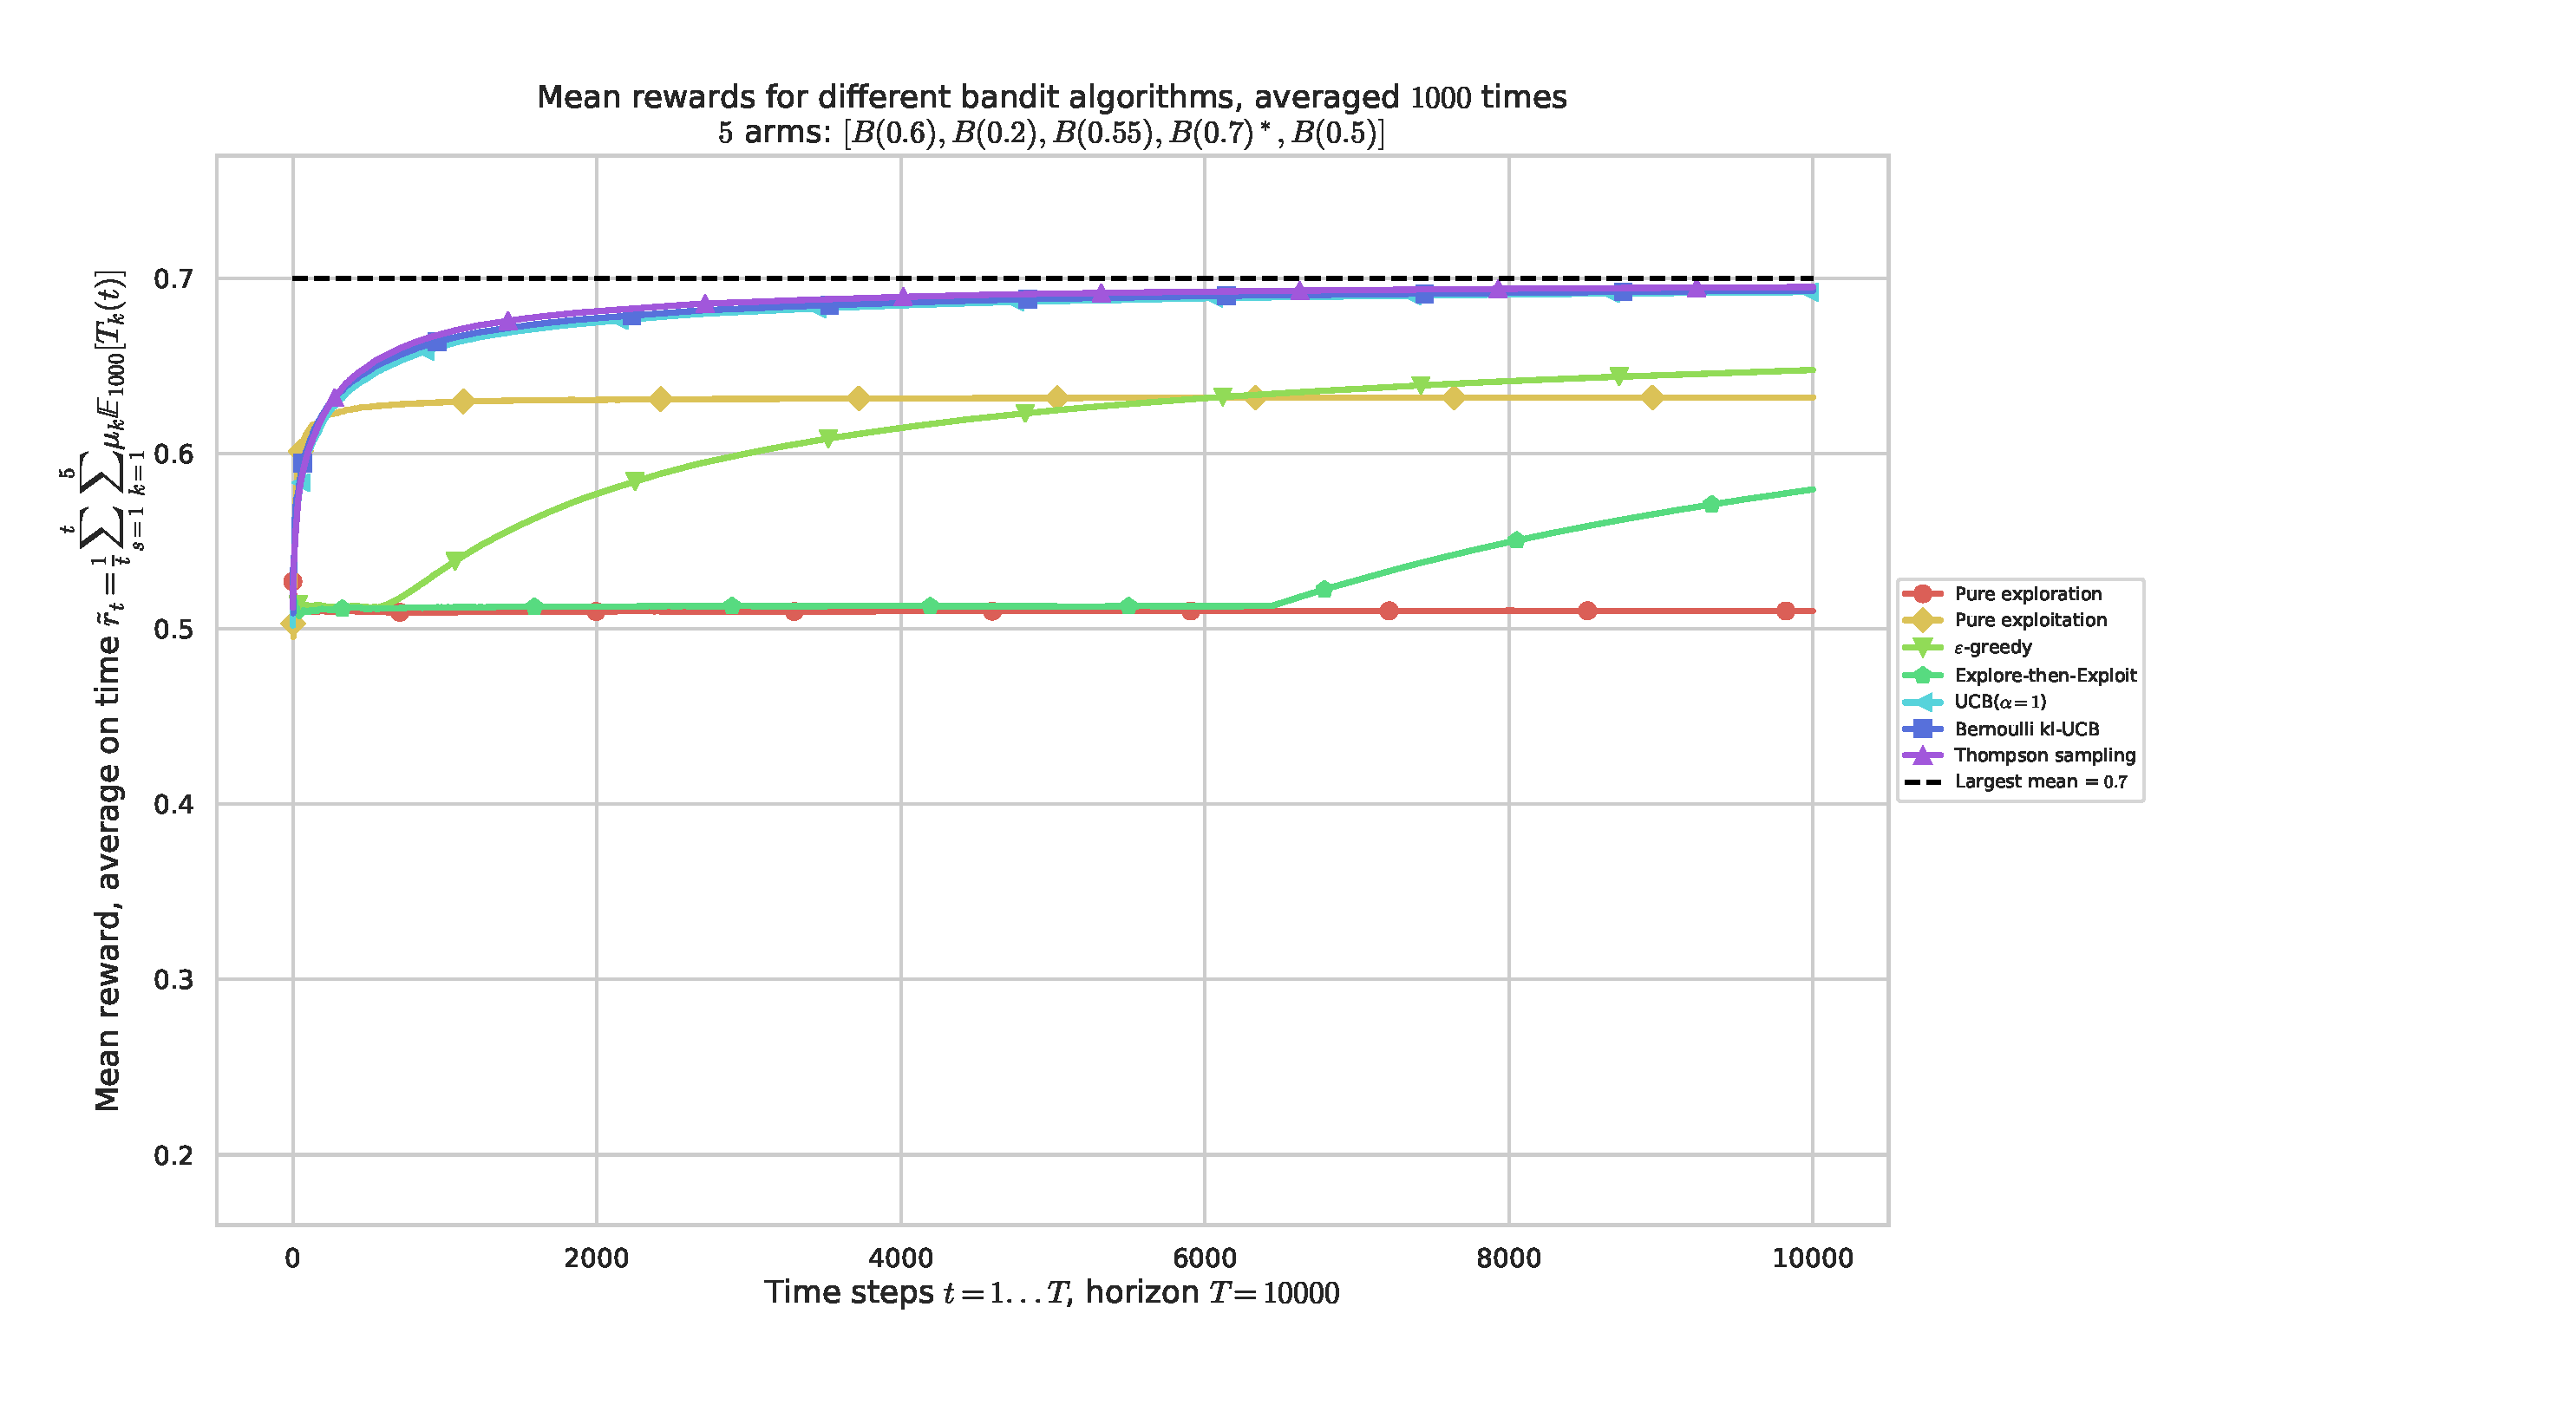
\includegraphics[width=1.15\linewidth]{SP__K5_T10000_N1000__7_algos/main_MeanRewards____env1-1_2506036032481767447.pdf}
	\caption{Average of the cumulated rewards, as function of $t$, for $T=10000$ and $N=1000$.}
	\label{fig:2:meanRewardsAsFunctionOfTimeForDifferentAlgorithmsT10000N1000}
\end{figure}

\begin{figure}[h!]  % [htbp]
	% \centering
	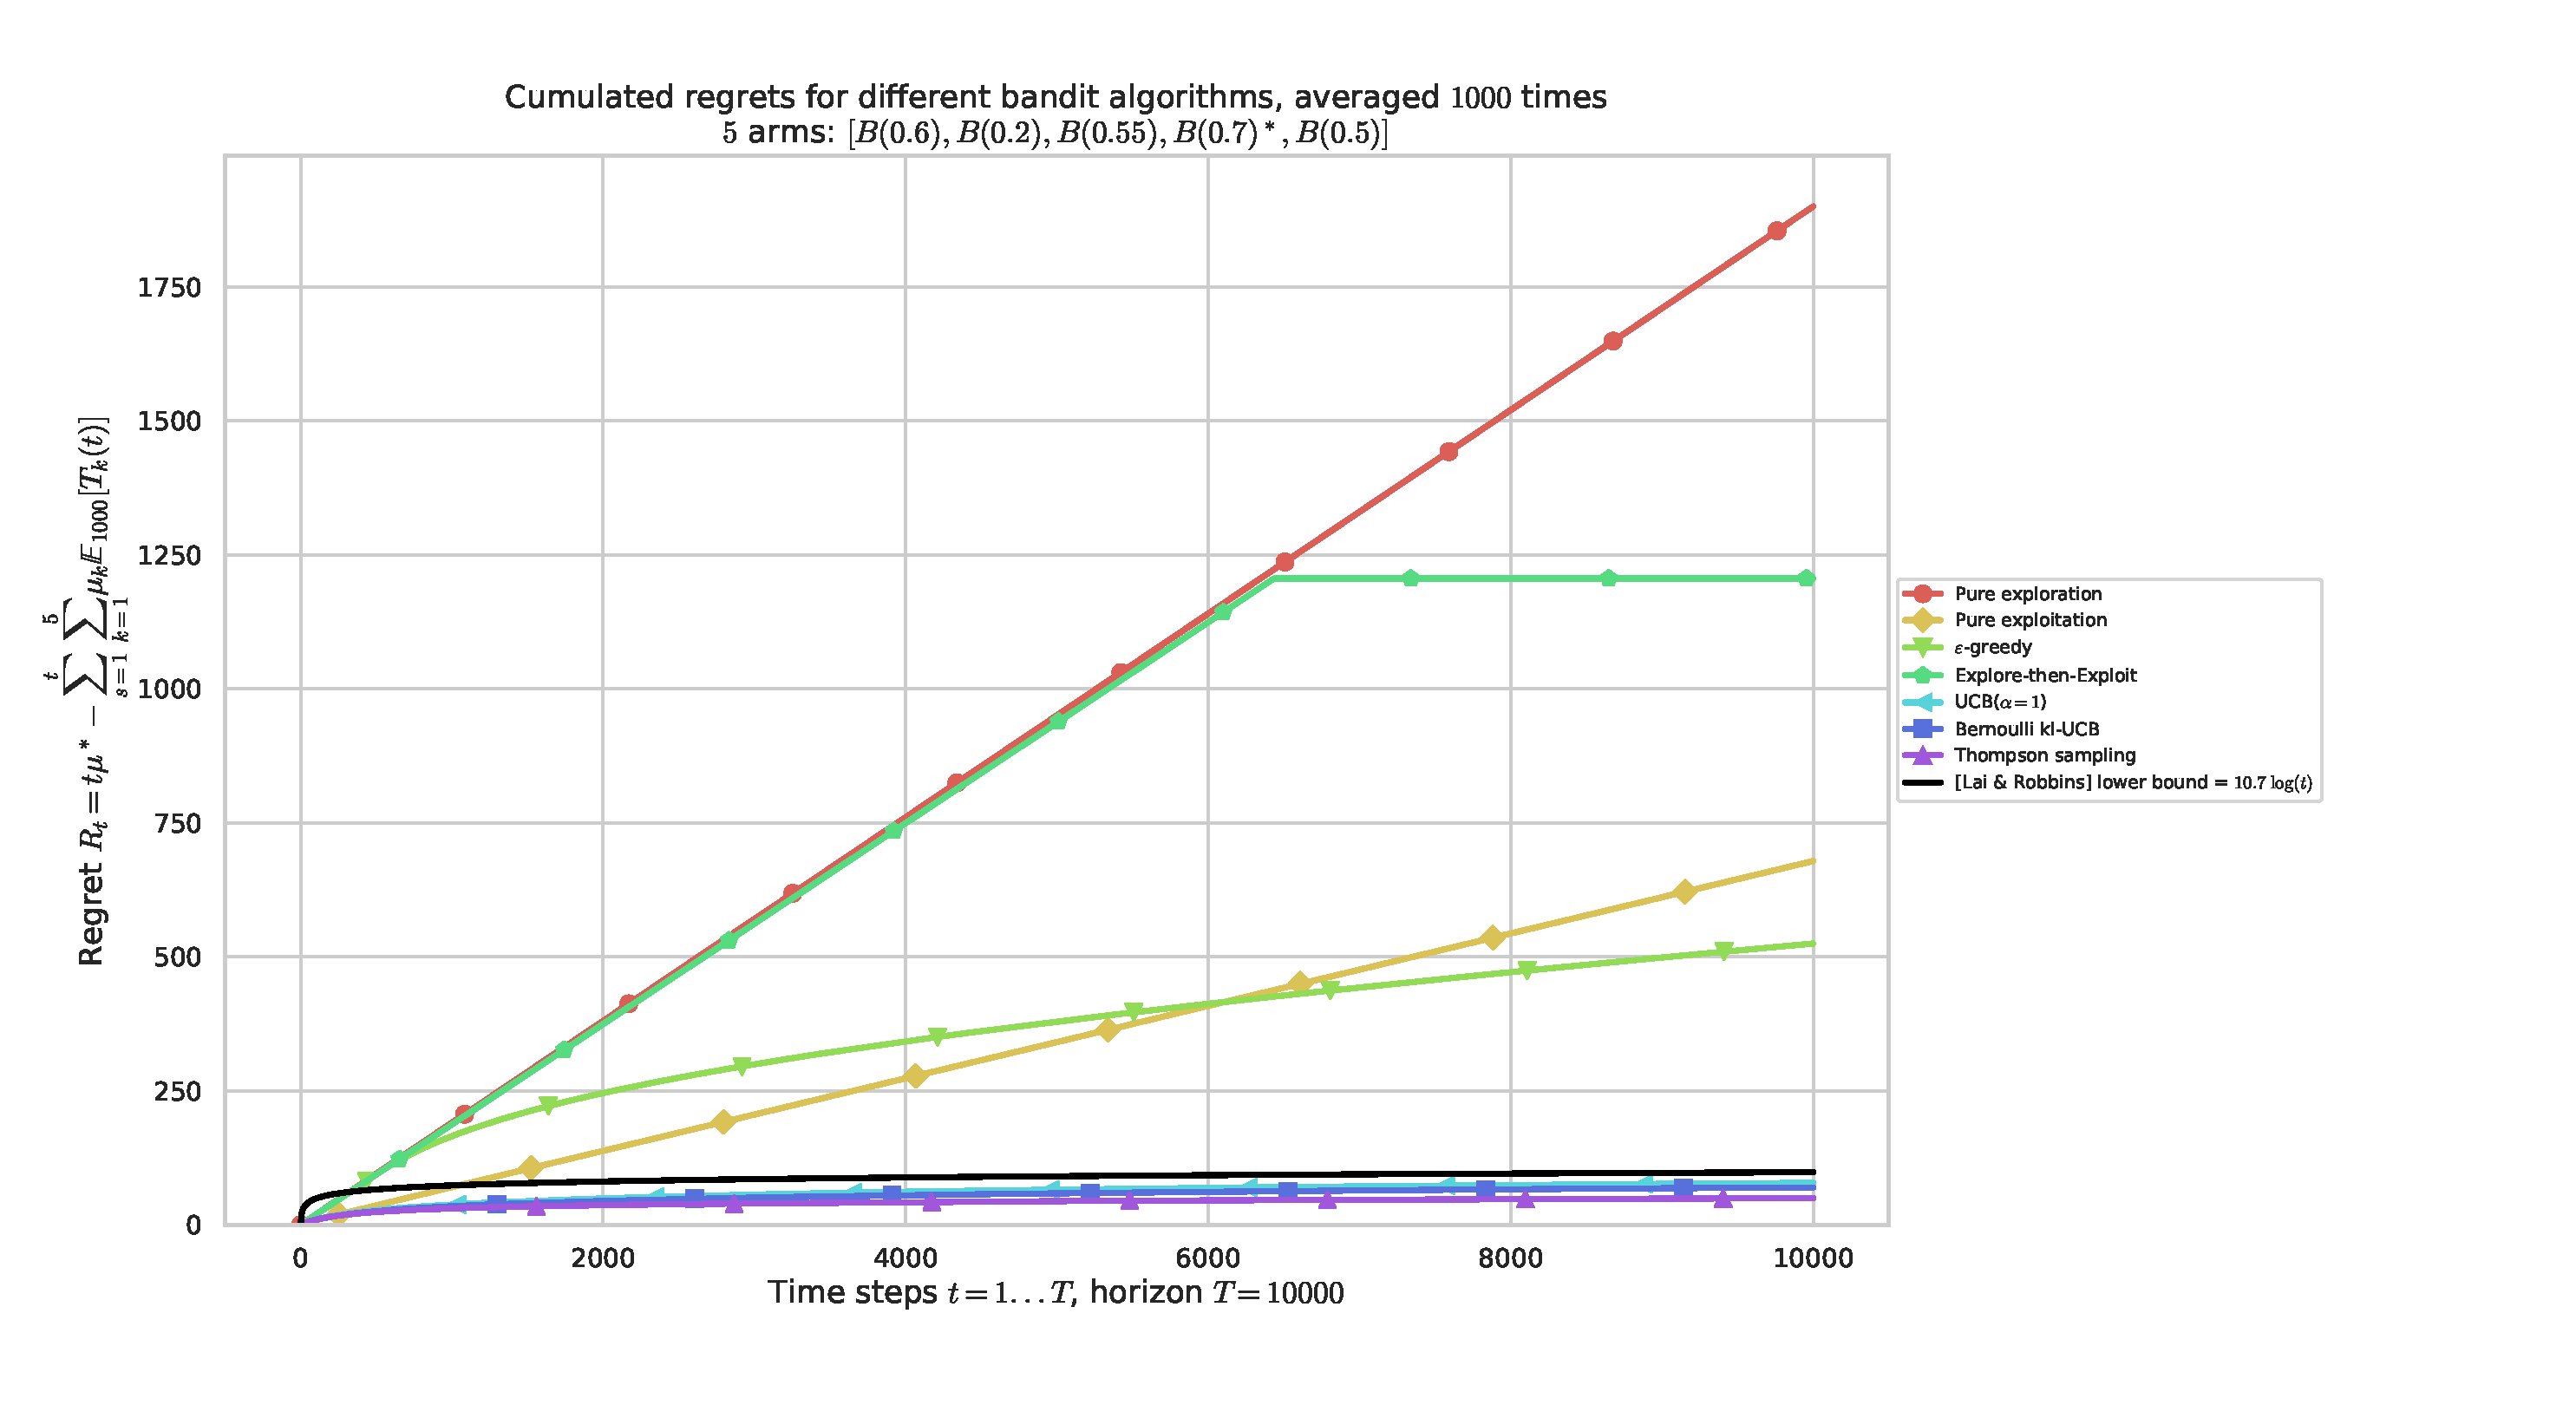
\includegraphics[width=1.15\linewidth]{SP__K5_T10000_N1000__7_algos/main____env1-1_2506036032481767447.pdf}
	\caption{Mean regret $R_t$ as function of $t$ for $T=10000$ and $N=1000$.}
	\label{fig:2:meanRegretAsFunctionOfTimeForDifferentAlgorithmsT10000N1000}
\end{figure}



\paragraph{Summary of this review of MAB algorithms.}
%
We gave an overview of the most well known families of algorithms for multi-armed bandits,
focussing on algorithms designed and analyzed for the single-player stationary and stochastic MAB model.
Except the naive and simple strategies given as introductory examples, most of the policies presented above are order-optimal for Bernoulli distributed problems or bounded rewards (or one-dimensional exponential families),
and some of them are known to be optimal in different settings.
%
To clearly understand the different in their empirical behaviors, we illustrated the performance of two naive and two simple strategies against three efficient ones, on the example of Bernoulli-distributed problem used for the online demonstration from Section~\ref{sec:2:notations} (see Figures~\ref{fig:2:example_of_a_5_arm_bandit_problem} and \ref{fig:2:example_of_a_5_arm_bandit_problem__step100}).
This also serves as a first example of numerical simulation performed with our library SMPyBandits, before the large-scale experiments of Section~\ref{sec:3:reviewSPAlgorithms} below.
%
In the rest of this thesis, we mainly use the $\UCB_1$ or Thompson sampling algorithms when simplicity and realistic deployment is favored (\ie, Chapter~\ref{chapter:4}), and the \klUCB{} algorithm when we give mathematical developments (\ie, Chapters~\ref{chapter:5} and \ref{chapter:6}).


% \newpage

% ----------------------------------------------------------------------------
\section{Different approaches on algorithm selection}
\label{sec:2:chooseYourPreferredBanditAlgorithm}

For any real-world applications of MAB algorithms,
several solutions have been explored based on various models, and for any model, typically there are many algorithms available, as we have seen above.
%
Thus, when a practitioner is facing a problem where MAB algorithms could be used, it is not an easy task to decide which algorithm to use.
It is hard to predict which solution could be the best for real-world conditions at every instant,
and even by assuming a stationary environment, when one is facing a certain problem but has limited information about it, it is hard to know beforehand which algorithm can be the best solution.

In this Section, we first present two naive approaches for selecting an algorithm when facing a new problem, and then we detail the online approach that uses a ``leader'' MAB algorithm running on top of a pool of ``followers'' algorithms, and we present our contribution that is a new ``leader'' algorithm based on \ExpQ.
This section is based on our article \cite{Besson2018WCNC}.


% ----------------------------------------------------------------------
\subsection{Motivation for online algorithm selection}\label{sub:25:introduction}

Many different learning algorithms have been proposed by the machine learning community,
and most of them depend on several parameters, for instance $\alpha$ for $\UCB_1$, the prior for Thompson sampling or BayesUCB,
the $\kl$ function for \klUCB{} etc.
Every time a new MAB algorithm $\Alg$ is introduced, it is compared and benchmarked on some bandit instances, parameterized by $\boldsymbol{\mu} = (\mu_1,\dots,\mu_K)$, usually by focusing on its expected regret $R_T^{\Alg}$.
%
For a known and specific instance, simulations help to select the best algorithm in a pool of algorithms,
but when one wants to tackle an \emph{unknown} real-world problem, one expects to be efficient against \emph{any} problem, of any size and complexity in a certain family:
ideally one would like to use an algorithm that can be applied identically against any problem of such family.


\textbf{Naive approaches:}
%
On the one hand, a practitioner can decide to pick one algorithm, maybe because it seems efficient on other problems, or maybe because it is simple enough to be used in its application. It might be unrealistic to implement complicated algorithms on limited hardware such as embedded chips in a very low-cost IoT end-device, and for instance a practitioner could chose to only consider the $\UCB_1$ algorithm (or other low-cost algorithms).
%
On the other hand, if prior knowledge on the application at hand is available, one could implement some benchmarks, and compare a set of algorithms on different problems. If a leader appears clearly, it is then possible to choose it for the application.


\textbf{Illustrative example:}
%
For instance, if you know that the considered problem can either have $K$ arms with very close means, or one optimal arm far away from the other, two versions of $\UCB_1$ will perform quite differently in the two problems:
using a large $\alpha$, \ie, favoring exploration, will give low regret in the first case,
while using a low $\alpha$, \ie, favoring exploitation, will give low regret in the second case.
One approach can be to use an intermediate value, as $\alpha=1/2$ suggested by theory, but another approach could be to consider an aggregated vote of different versions of $\UCB_1$, each running with a different value of $\alpha$ (\eg, in a logarithmic grid), and let another learning algorithm decide which value of $\alpha$ is the best \emph{for the problem at hand}.

\textbf{The online approach:}
%
Another possibility is to consider an online approach, which is interested in the case where the computation power or memory storage of the application is not a limitation factor, but where one cannot run benchmarks before deploying the application.
We consider a fixed set of algorithms, and we use another learning algorithm on top of this set, to learn \emph{on the fly} which one should be trusted more, and eventually, used on its own.

The aggregation approach is especially interesting if we know that the problem the application will face is one of a few known kinds of problems.
In such cases, if there are $N$ different sorts of problems, and if the practitioner has prior knowledge on it, one can use the naive approach to select an algorithm $\cA_i$ which should perform well on problem $i$, for $i\in[N]$,
and use the aggregation of $\cA_1,\dots,\cA_N$ when facing the unknown problem.

% To choose the best algorithm, three approaches can be followed:
% \begin{itemize}
%     \item
% \end{itemize}
% either extensive benchmarks are done beforehand -- if this is possible -- to select the algorithm and its optimal parameters, or an adaptive algorithm is used to learn \emph{on the fly} its parameters.

% We present a simple adaptive solution, that aggregates several learning algorithms in parallel and adaptively chooses which one to trust the most.

% \paragraph{Outline.}
% This section is organized as follows.
% First, we explain in Section~\ref{sub:25:aggregation} how to combine such algorithms for aggregation.
% Then we present our proposed algorithm, called \Aggr, in Section~\ref{sub:25:Aggr},
% Finally, we present numerical experiments in Section~\ref{sub:25:numExp},
% on Bernoulli and non-Bernoulli MAB problems,
% comparing the regret of several algorithms against different aggregation algorithms.
% Theoretical guarantees are shortly discussed in Section~\ref{sub:25:theory}, and Section~\ref{sub:25:conclusion} concludes.


% \subsection{Naive approaches}

% As mentioned, there are two naive approaches

% use UCB or Thompson sampling, and forget about the rest!}
% First solution: be naive, only use UCB everywhere


% \subsection{Use prior knowledge about the future application to select beforehand the chosen algorithm}

% Second solution, if one has some prior knowledge about the domain or setting for which the learning algorithms will be deployed, she can run synthetic or real-world simulations, compare many algorithms before deployment, and select the best algorithm!


\subsection{Online algorithm selection with expert aggregation}

% - ``Aggregation of Multi-Armed Bandits learning algorithms for Opportunistic Spectrum Access'', see https://hal.inria.fr/hal-01705292

As we said, a third possible approach is to select \emph{on the run} the best algorithm for a specific situation, for which the so called \emph{expert aggregation algorithms} framework can be useful.
%
To the best of our knowledge, aggregation algorithms, such as \ExpQ{} which dates back from 2002 \cite{Auer02},
have never been used in pratice for stochastic MAB problems.
% and we show that it appears empirically sub-optimal when applied to simple stochastic problems.

We present an improved variant of \ExpQ, called \Aggr.
For synthetic MAB problems, with Bernoulli or other distributions for $K$ arms, simulation results are presented to demonstrate its empirical efficiency.
We combine classical algorithms, such as Thompson sampling, Upper-Confidence Bounds algorithms (\UCB{} and variants), and Bayesian or Kullback-Leibler UCB.
%
Our algorithm offers good performance compared to state-of-the-art algorithms
(\ExpQ{}, \CORRAL{} or \LearnExp{}) \cite{Agarwal16,Singla17},
and appears as a robust approach to select on the run the best algorithm for any stochastic MAB problem, being more realistic to real-world radio settings than any tuning-based approach.

% \TODOL{This chapter is basically a raw include from my paper ``Aggregation of Multi-Armed Bandits learning algorithms for Opportunistic Spectrum Access'', see https://hal.inria.fr/hal-01705292}


% ----------------------------------------------------------------------
% \subsection{Aggregating bandit algorithms}\label{sub:25:aggregation}
\paragraph{Notations}\label{sub:25:aggregation}

We assume to have $N \geq 2$ MAB algorithms, $\Alg_1, \dots, \Alg_N$,
and let $\Alg_{\mathrm{aggr}}$ be an aggregation algorithm,
which runs the $N$ algorithms in parallel (with the same slotted time), and use them to choose its channels based on a voting from their $N$ decisions.
%
$\Alg_{\mathrm{aggr}}$ depends on a pool of algorithms and a set of parameters.
We would like that $\Alg_{\mathrm{aggr}}$
performs almost as well as the best of the $\Alg_a$, with a good choice of its parameters, independently of the MAB problem.
Ideally $\Alg_{\mathrm{aggr}}$ should perform similarly to the best of the $\Alg_a$.
%
To simplify the presentation, we only aggregate bandit algorithms that give deterministic recommendations:
one arm is chosen with probability $1$ and the others with probability $0$.
However, both \ExpQ{} and \Aggr{} can be adapted to aggregate randomized bandit algorithms, \ie, algorithms that output a probability distribution $\xi_t$ over the arms $[K]$ at each time step, and draw the next selected arm according to this distribution
(\eg, Thompson sampling).

The aggregation algorithm maintains a probability distribution $\pi^{t}$ on the $N$ algorithms $\Alg_a$, starting from a uniform distribution:
$\pi^t_a$ is the probability of trusting the decision made by algorithm $\Alg_a$ at time $t$.
$\Alg_{\mathrm{aggr}}$ then simply performs a weighted vote on its algorithms: it decides whom to trust by sampling $a \in [N]$ from $\pi^t$, then follows $\Alg_a$'s decision.
The main questions are then to know what observations (\ie, arms and rewards) should be given as feedback to which algorithms,
and how to update the trusts at each step, and our proposal \Aggr{} differs from \ExpQ{} on these very points.


% ----------------------------------------------------------------------
\subsection{Our contribution: the \Aggr{} algorithm}\label{sub:25:Aggr}

Our proposed \Aggr{} is detailed in Algorithm~\ref{algo:25:Aggr}.
%
\begin{small}
	\begin{figure}[h!]
		\centering
		\begin{framed}
		% Documentation at http://mirror.ctan.org/tex-archive/macros/latex/contrib/algorithm2e/doc/algorithm2e.pdf if needed
		% Or https://en.wikibooks.org/wiki/LaTeX/Algorithms#Typesetting_using_the_algorithm2e_package
		\begin{algorithm}[H]
			% XXX Input, data and output
			\KwIn{$N$ bandit algorithms, $\Alg_1, \dots, \Alg_N$, with $N \geq 2$}
			\KwIn{Number of arms, $K \geq 2$}
			\KwIn{Time horizon, $T \geq 1$, \textbf{not} used for the learning}
			\KwIn{A sequence of learning rates, $(\eta_t)_{t \geq 1}$}
			\KwData{Initial uniform distribution, $\pi^{0} = \cU([N])$}
			\KwResult{$\Alg_{\mathrm{aggr}}=\Aggr\left[\Alg_1, \dots, \Alg_N\right]$}
			% XXX Algorithm
			\For(\tcp*[f]{At every time step})
            {$t = 1, \dots, T$}{
				%
				% \tcp{First, run each algorithm $\Alg_a$}
				\For(\tcp*[f]{Can be parallel}){$a = 1, \dots, N$}{
					$\Alg_a$ updates its internal state (e.g., \UCB{} indexes)\;
					It chooses $A(t+1)_{a} \in [K]$.
				}
				%
				% \tcp{The more algorithms have chosen arm $j$, the more probable it is to be chosen.}
				Let $p^{t+1}_j := \sum\limits_{a = 1}^{N} \pi^{t}_a \times \mathbbm{1}(\{A(t+1)_{a} = j\}), \;\forall 1\leq j \leq K$\;
				% \tcp*{Sum trusts}
				Then $\Alg_{\mathrm{aggr}}$ chooses arm $A(t+1) \sim p^{t+1}$\;
				% $\P(A(t+1)_{\mathrm{aggr}} = j) = p^{t+1}_j$
				% \tcp*{Sample once}
				%
				Give \emph{original} reward $(A(t+1), 1 - \ell_{A(t+1)}(t+1))$ to \emph{each} $\Alg_a$ (maybe \emph{not} on its chosen arm)\;
				Compute an \emph{unbiased} estimate of the loss of the trusted algorithms,$$ \ell^{t+1} = \ell_{A(t+1)}(t+1) / p^{t+1}_{A(t+1)}\;. $$
				% \tcp{Use bandit feedback to update $\pi^{t}$}
				% \tcp{Finally, use the instantaneous bandit feedback (loss $\ell_{A(t+1),t}$) to update $\pi^{t}$}
				% \For(\tcp*[f]{Can be parallel}){$a = 1, \dots, N$}{
				\For{$a = 1, \dots, N$}{
					% \eIf{$\Alg_a$ was trusted, \ie, $A(t+1)_{a} = A(t+1)$}{
					\If{$\Alg_a$ was trusted, \ie, $A(t+1)_{a} = A(t+1)$}{
						$ \pi^{t+1}_{a} = \exp(\eta_t \ell^{t+1}) \times \pi^{t}_{a} $
						% \tcp*{More trusted}
						}%{
						% $ \pi^{t+1}_{a} = \exp(- \eta_t \ell^{t+1}) \times \pi^{t}_{a} $
						% \tcp*{Less trusted}
					% }
				}
				Renormalize the new $\pi$: $\pi^{t+1} := \pi^{t+1} / \sum_{a=1}^{N} \pi^{t+1}_{a}$.
				% \tcp*{Project it back to $\Delta_N$}
			}
			\caption{Our aggregation algorithm \Aggr.}
			\label{algo:25:Aggr}
		\end{algorithm}
		\end{framed}
	\end{figure}
\end{small}


At every time step, after having observed a loss $\ell_{A(t+1)}(t+1)$ for its chosen action $A(t+1)$,
the algorithm updates the trust probabilities from $\pi^t$ to $\pi^{t+1}$ by
a multiplicative exponential factor (using the learning rate and the \emph{unbiased} loss).
%
Only the algorithms $\Alg_a$ who advised the last decision get their trust updated, in order to trust more the ``reliable'' algorithms.

The loss estimate is unbiased in the following sense. If one had access to the rewards $r_k(t+1)$ (or the losses $\ell_k(t+1)$) for all arms $k$, the loss incurred by algorithm $a$ at time $t+1$ would be $\tilde{\ell}_{a,t+1} = \ell_{A_A(t+1)}(t+1)$. This quantity can only be observed for those algorithms for which $A_{a}^{t+1}=A(t+1)$. However, by dividing by the probability of observing this recommendation, one obtains an unbiased estimate of $\tilde{\ell}_{a,t}$. More precisely, if we define the estimate by
\begin{equation}
	\hat{\ell}_{a,t+1} = \frac{\ell_{A_A(t+1)}(t+1)}{p_{A_A(t+1)}^{t+1}} \mathbbm{1}(A_A(t+1) = A(t+1))
\end{equation}
satisfies $\mathbb{E}[\hat{\ell}_{a,t+1} | \mathcal{H}_t] = \tilde{\ell}_{a,t+1}$, for all $a$, where the expectation is taken conditionally to the history of observations up to round $t$, $\mathcal{H}_{t}$. Observe that $\tilde{\ell}_{a,t+1}=\ell^{t+1}$ for all algorithms $a$ such that $A_A(t+1)=A(t+1)$, and $\tilde{\ell}_{a,t+1}=0$ otherwise.


% - Precise some tricky points
An important feature of \Aggr{} is the feedback provided to each underlying bandit algorithm, upon the observation of arm $A(t+1)$. Rather than updating only the trusted algorithms (that is the algorithms which would have drawn arm $A(t+1)$) with the observed reward $r_{A(t+1)}(t+1)=1 - \ell_{A(t+1)}(t+1)$,  we found that updating each algorithm with the (original) loss observed for arm $A(t+1)$ improves the performance drastically.
%
As expected, the more feedback they get, the faster the underlying algorithms learn, and the better the aggregation algorithm is.
This intuition is backed up by theory explained in \cite{Maillard11}.


Regarding the update of $\pi^t$, one can note that the trust probabilities are not all updated before the normalization step,
and an alternative would be to
increase $\pi_{a}$ if $A(t+1)_a = A(t+1)$ and to decrease it otherwise.
It would not be so different, as there is a final renormalization step, and empirically this variation has little impact on the performance of \Aggr{}.



% ----------------------------------------------------------------------
\subsubsection{Explanations of \Aggr{} versus \ExpQ{} }\label{sub:25:Exp4}

% - explain, but don't give pseudo-code ?
The \ExpQ{} algorithm (see, e.g. \cite[Section 4.2]{Bubeck12})
is similar to \Aggr{}, presented in Algorithm \ref{algo:25:Aggr},
but differs in the two following points.
%
First, $a\sim\pi^t$ is sampled first and the arm chosen by $\Alg_a$ is trusted, whereas \Aggr{}
needs to listen to the $N$ decisions to perform the updates on $\pi^{t+1}$.
Then, \ExpQ{} gives back an observation (arm, reward) only to the last trusted algorithm
whereas \Aggr{} gives it to all algorithms.
%
Second, after having computed the loss estimate $\ell$, \ExpQ{} updates the estimated cumulative loss for each algorithm,
$\widetilde{L}_a(t) = \sum_{s=1}^{t} \ell_{A_a^s}(s) \times \mathbbm{1}(A^{s}_{a} = A^{s}_{\mathrm{aggr}})$.
%
Instead
\footnote{~It is the same for constant learning rates, and does not differ much for decreasing learning rates.}
of updating $\pi^{t}$ multiplicatively as we do for our proposal, \ExpQ{} recomputes it, proportionally to
$\exp(- \eta_t \widetilde{L}_a(t))$.


\paragraph{How to choose the learning rates $(\eta_t)$?}
%
The sequence of non-negative learning rates $(\eta_t)_{t \geq 1}$ used by \ExpQ{} can be arbitrary.
It can be constant but should be non-increasing \cite[Theorem 4.2]{Bubeck12}.
% helps to choose a good sequence.
If the horizon $T$ is known (and fixed), the best choice is given by $\eta_t = \eta = 2 \log(N) / (T K)$.
However, for real-world communication problems, it can be considered unrealistic\footnote{~For more discussion on this hypothesis, we refer to Section~1 of our article \cite{Besson2018DoublingTricks}.} to assume a fixed and known time horizon, so we prefer the alternative horizon-free choice%
\footnote{~It is non-increasing, and is obtained by minimizing the upper-bound on the regret derived in \cite[pp48]{Bubeck12}.}
of learning rates,
$\eta_t = \log(N) / (t K)$ suggested by \cite{Bubeck12}.
We compare both approaches empirically, and the second one usually performs better.
We also stick to this choice of $(\eta_t)_{t \geq 1}$ for \Aggr.



% ----------------------------------------------------------------------
\subsection{Experiments on simulated MAB problems}\label{sub:25:numExp}

% \TODOL{Je pense refaire complètement les expériences de ce morceau.

% - C'est un peu bête de montrer des problèmes chelous genre Gaussien et "mixed" quand tout le reste de la thèse s'intéresse vraiment aux Bernoulli.

% - C'est un peu naze de montrer en log-y ou en log-log, alors que le reste de la thèse s'intéresse uniquement à des plots x-y, ou des histogrammes.

% - Pour être plus consistant avec les sections suivantes, je pourrais inclure juste 1/2 courbes de regret, et un tableau de résultats pour d'autres problèmes ?
% }

% - explain the problem studied in the simulation
We focus on \emph{i.i.d.} MAB problems, with $K = 9$ channels\footnote{~Similar behaviors are observed for any not-too-large values of $K$, we tried up-to $K = 100$ and the same results were obtained.}.
For Bernoulli problem, the first one uses $\boldsymbol{\mu}=[0.1,\dots,0.9]$, and is considered as a ``simple'' problem.
The second one is divided in three groups:
2 very bad arms ($\mu = 0.01, 0.02$), 5 average arms ($\mu = 0.3$ to $0.6$) and 3 very good arms ($\mu = 0.78, 0.8, 0.82$), and it is considered as a ``harder'' problem.
The horizon is set to $T = 20000$ (but its value is unknown to all algorithms), and simulations are repeated $1000$ times, to estimate the expected regret.
%
This empirical estimation of the expected regret $R_T$ is plotted below, as a function of $T$, comparing some algorithms $\Alg_1,\dots,\Alg_N$ (for $N=6$), and their aggregation with \Aggr{} (displayed in orange bold),
using the parameter-free learning rate sequence, $\eta_t = \log{N} / (t K)$.

The Lai \& Robbins' logarithmic lower-bound \cite{LaiRobbins85} is also plotted.
It corresponds to the second point \eqref{eq:2:forSecondLogTLowerBound2} in Theorem~\ref{thm:2:secondLogTLowerBound}.
It is crucial to note that the lower-bound is only asymptotic, and as such one should not be surprised to see regret curves smaller than the lower-bound (\eg, for the easier Bernoulli problem in Figure~\ref{fig:25:EasyBernoulli}).

Note that for each of the $1000$ simulations, we choose to generate all the rewards beforehand, \ie, one full matrix $(r_k(t))_{1\leq k \leq K, 1 \leq t \leq T}$ for every repetition, in order to compare the algorithms on the same realizations%
\footnote{Similar plots and similar results are obtained if this choice is not made, but it makes more sense to compare them against the same randomization. Note that this choice is the default in SMPyBandits, but the other possibility is implemented as well, by changing \texttt{cache\_rewards} to \texttt{true} or \texttt{false} in the \texttt{configuration} dictionary. See Section~\ref{sub:3:miniConfigurationFileSMPyBandits} for explanations on this \texttt{configuration.py} file, or the online documentation.}
of the MAB problem.

We compare our \Aggr{} algorithm,
as well as other aggregation algorithms, \ExpQ{} from \cite{Bubeck12},
\CORRAL{} from \cite{Agarwal16} and \LearnExp{} from \cite{Singla17}, all with their default parameters.
%
The aggregated algorithms consist in a naive uniform exploration (to have at least one algorithm with bad performances, \ie, linear regret, but it is not included in the plots),
\UCB{} with $\alpha=1/2$, three \klUCB{} algorithms respectively using Bernoulli, Gaussian and exponential $\kl$ functions, and BayesUCB and Thompson sampling with uniform prior.

Figures~\ref{fig:25:EasyBernoulli} and \ref{fig:25:HarderMixed} are in semilog-$y$ scale, this helps to see that the best algorithms can be an \emph{order of magnitude} more efficient than the worst, and the \Aggr{} performs similarly to the best ones, when the other aggregation algorithms are usually amongst the worst.
Figure~\ref{fig:25:HarderMixed_semilogx} is in semilog-$x$ scale to show that the regret of efficient algorithms are indeed logarithmic.


\begin{figure}[h!]  % [htbp]
	\centering
	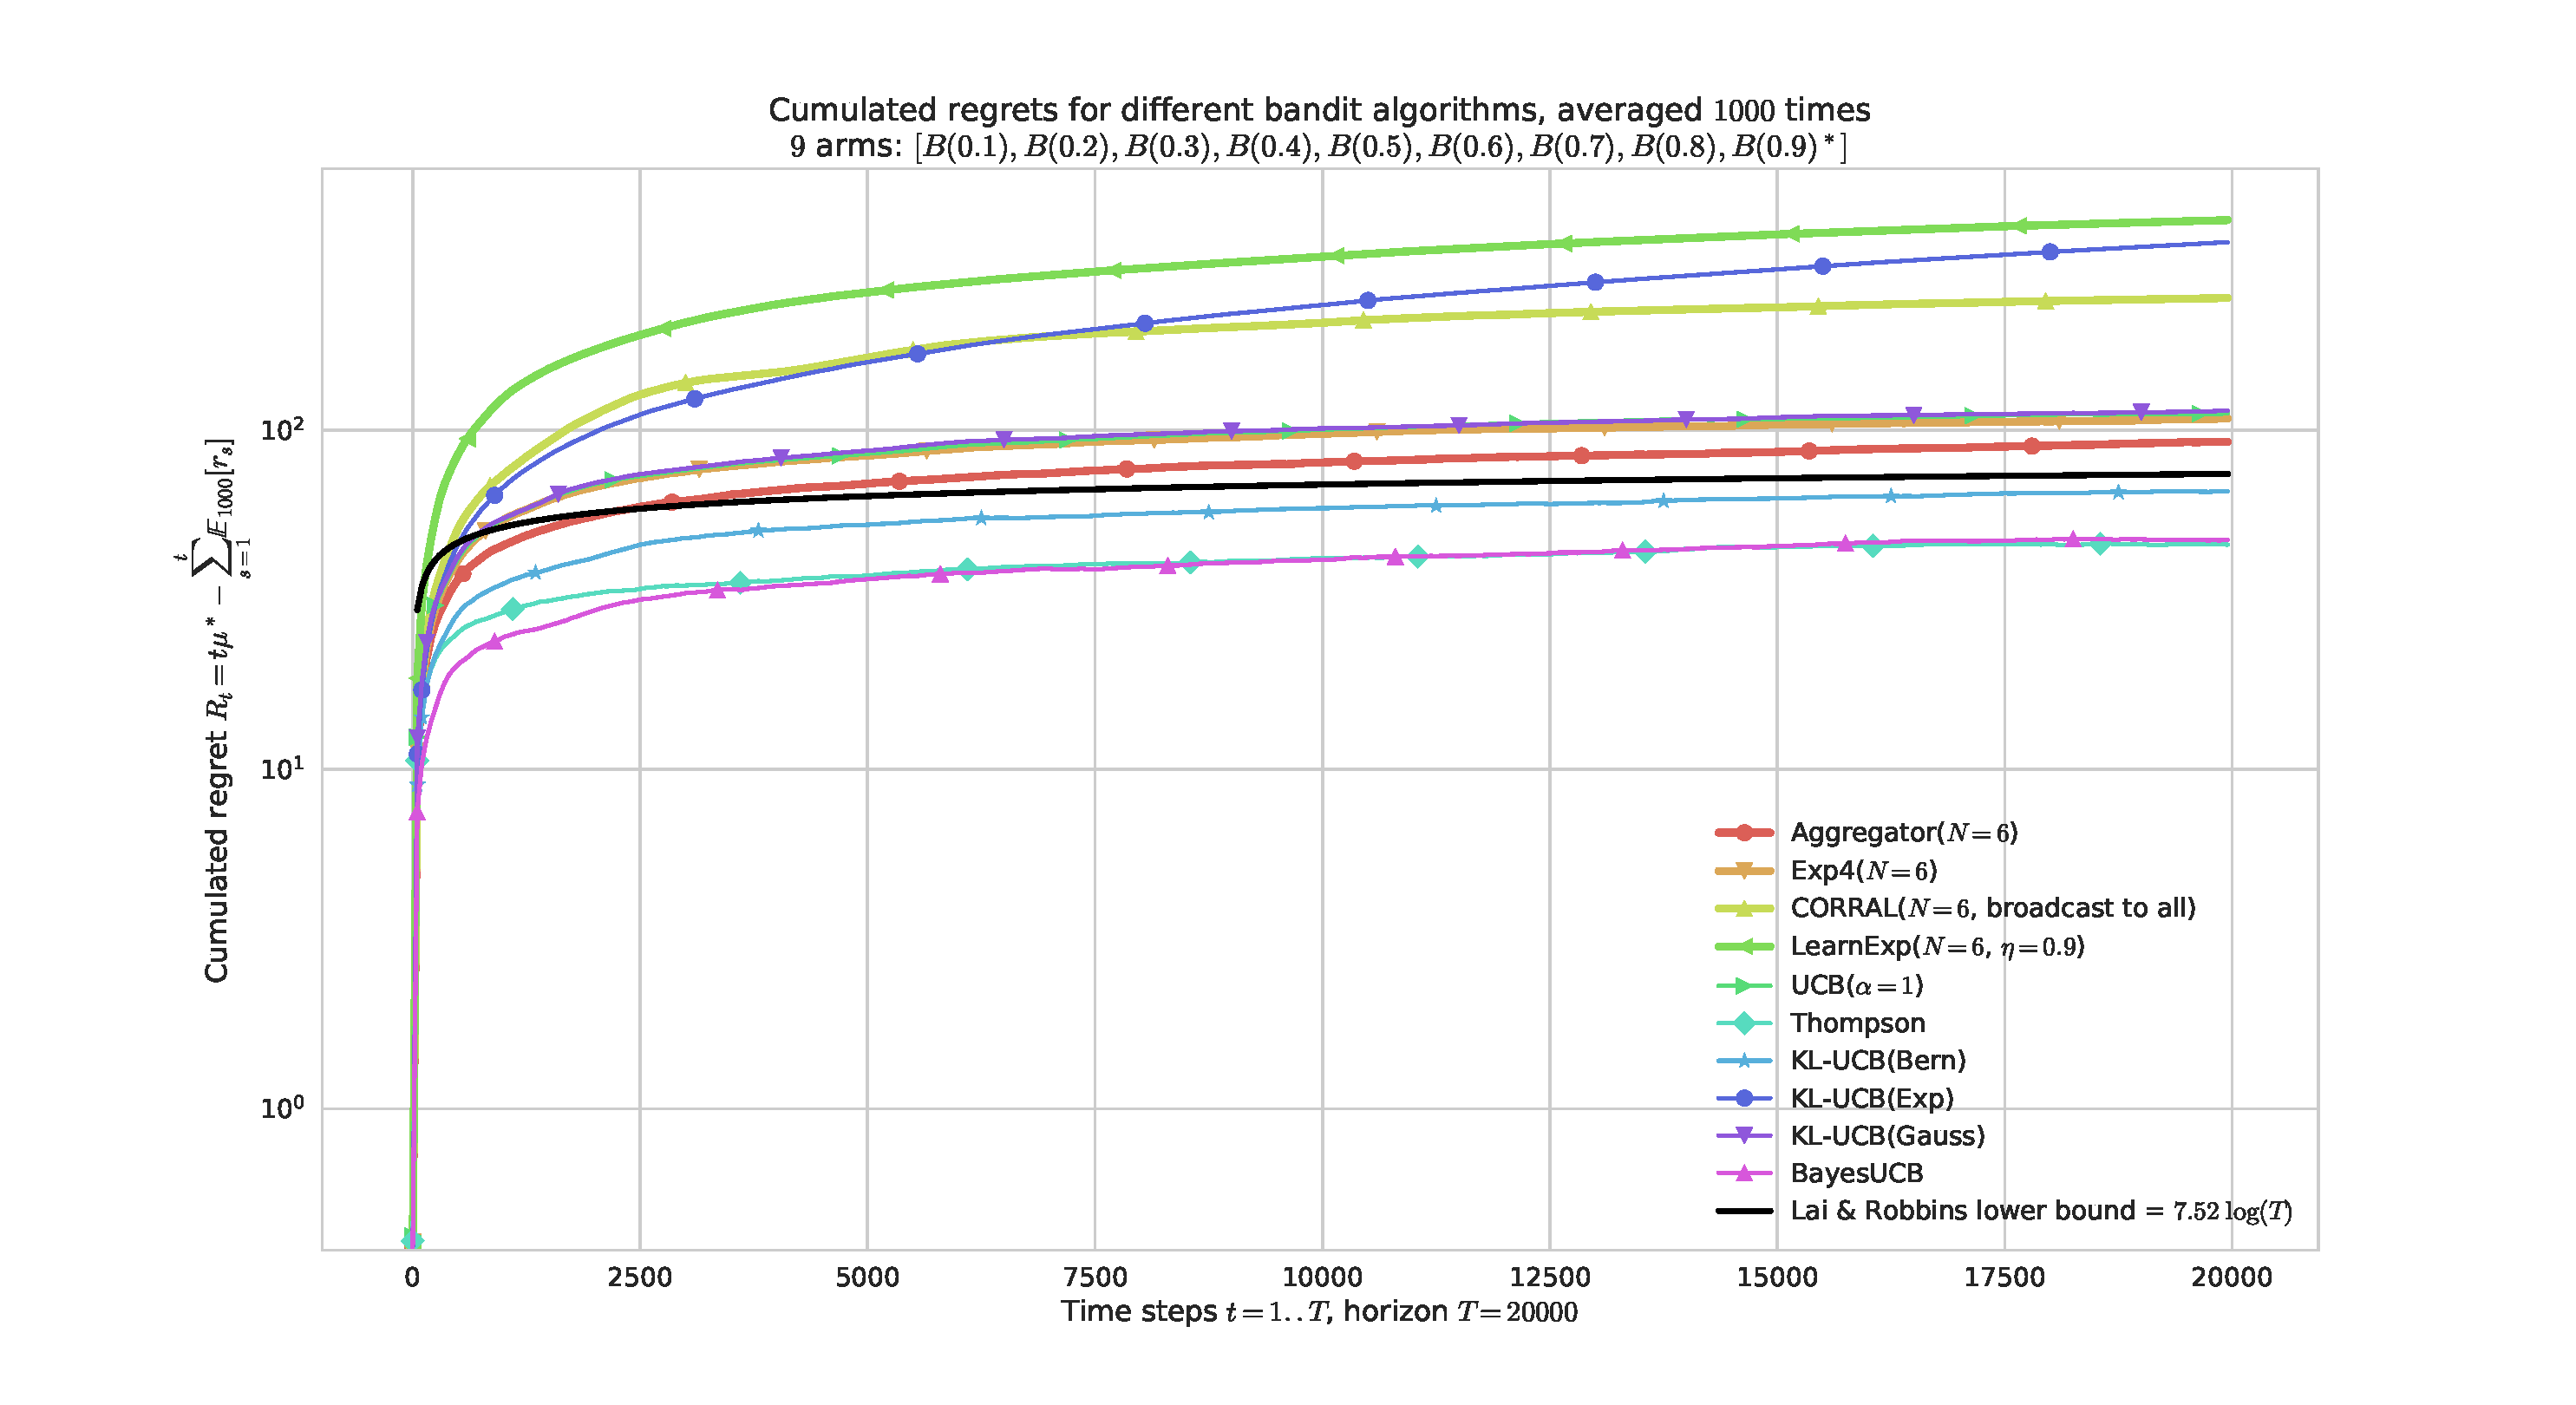
\includegraphics[width=1.10\linewidth]{2-Chapters/2-Chapter/IEEE_WCNC_2018.git/plots/main_semilogy____env1-4_932221613383548446.pdf}
	\caption{On a ``simple'' Bernoulli problem (semilog-$y$ scale).}
	\label{fig:25:EasyBernoulli}
\end{figure}

\begin{figure}[b!]  % [htbp]
	\centering
	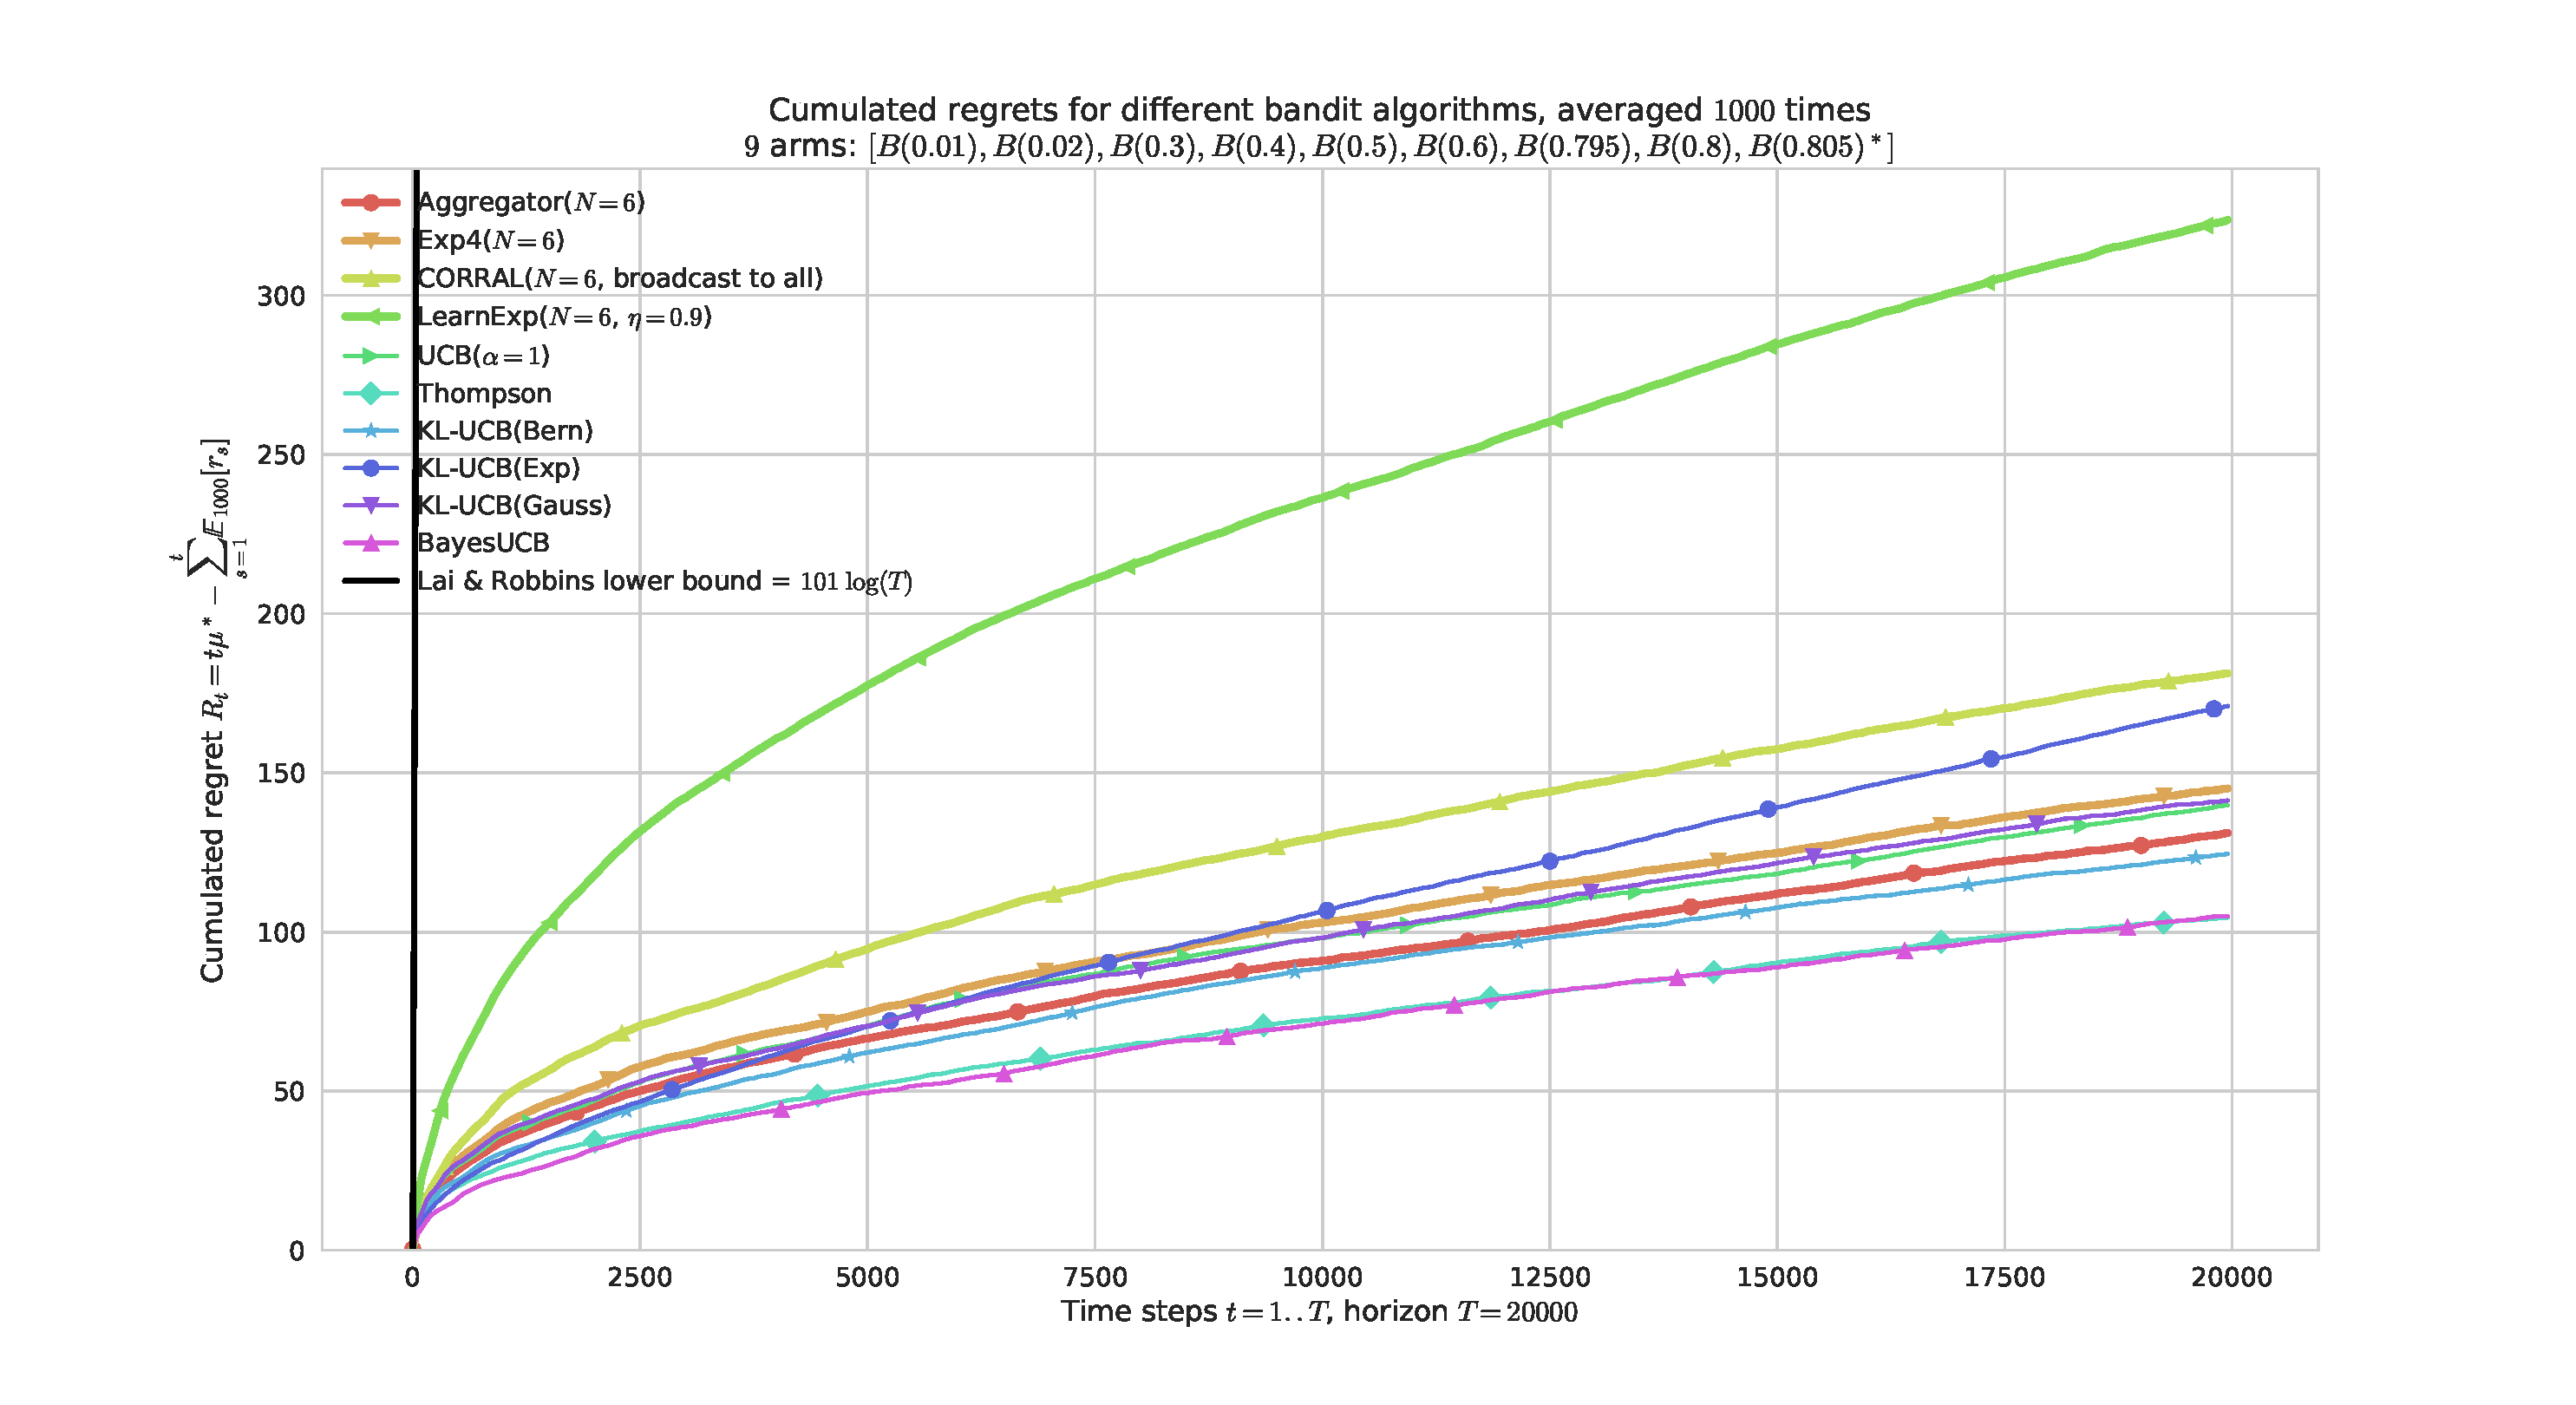
\includegraphics[width=1.10\linewidth]{2-Chapters/2-Chapter/IEEE_WCNC_2018.git/plots/main____env2-4_932221613383548446.pdf}
	\caption{On a ``harder'' Bernoulli problem, they all have similar performances, except \LearnExp.}
	\label{fig:25:HardBernoulli}
\end{figure}

\begin{figure}[b!]  % [htbp]
	\centering
	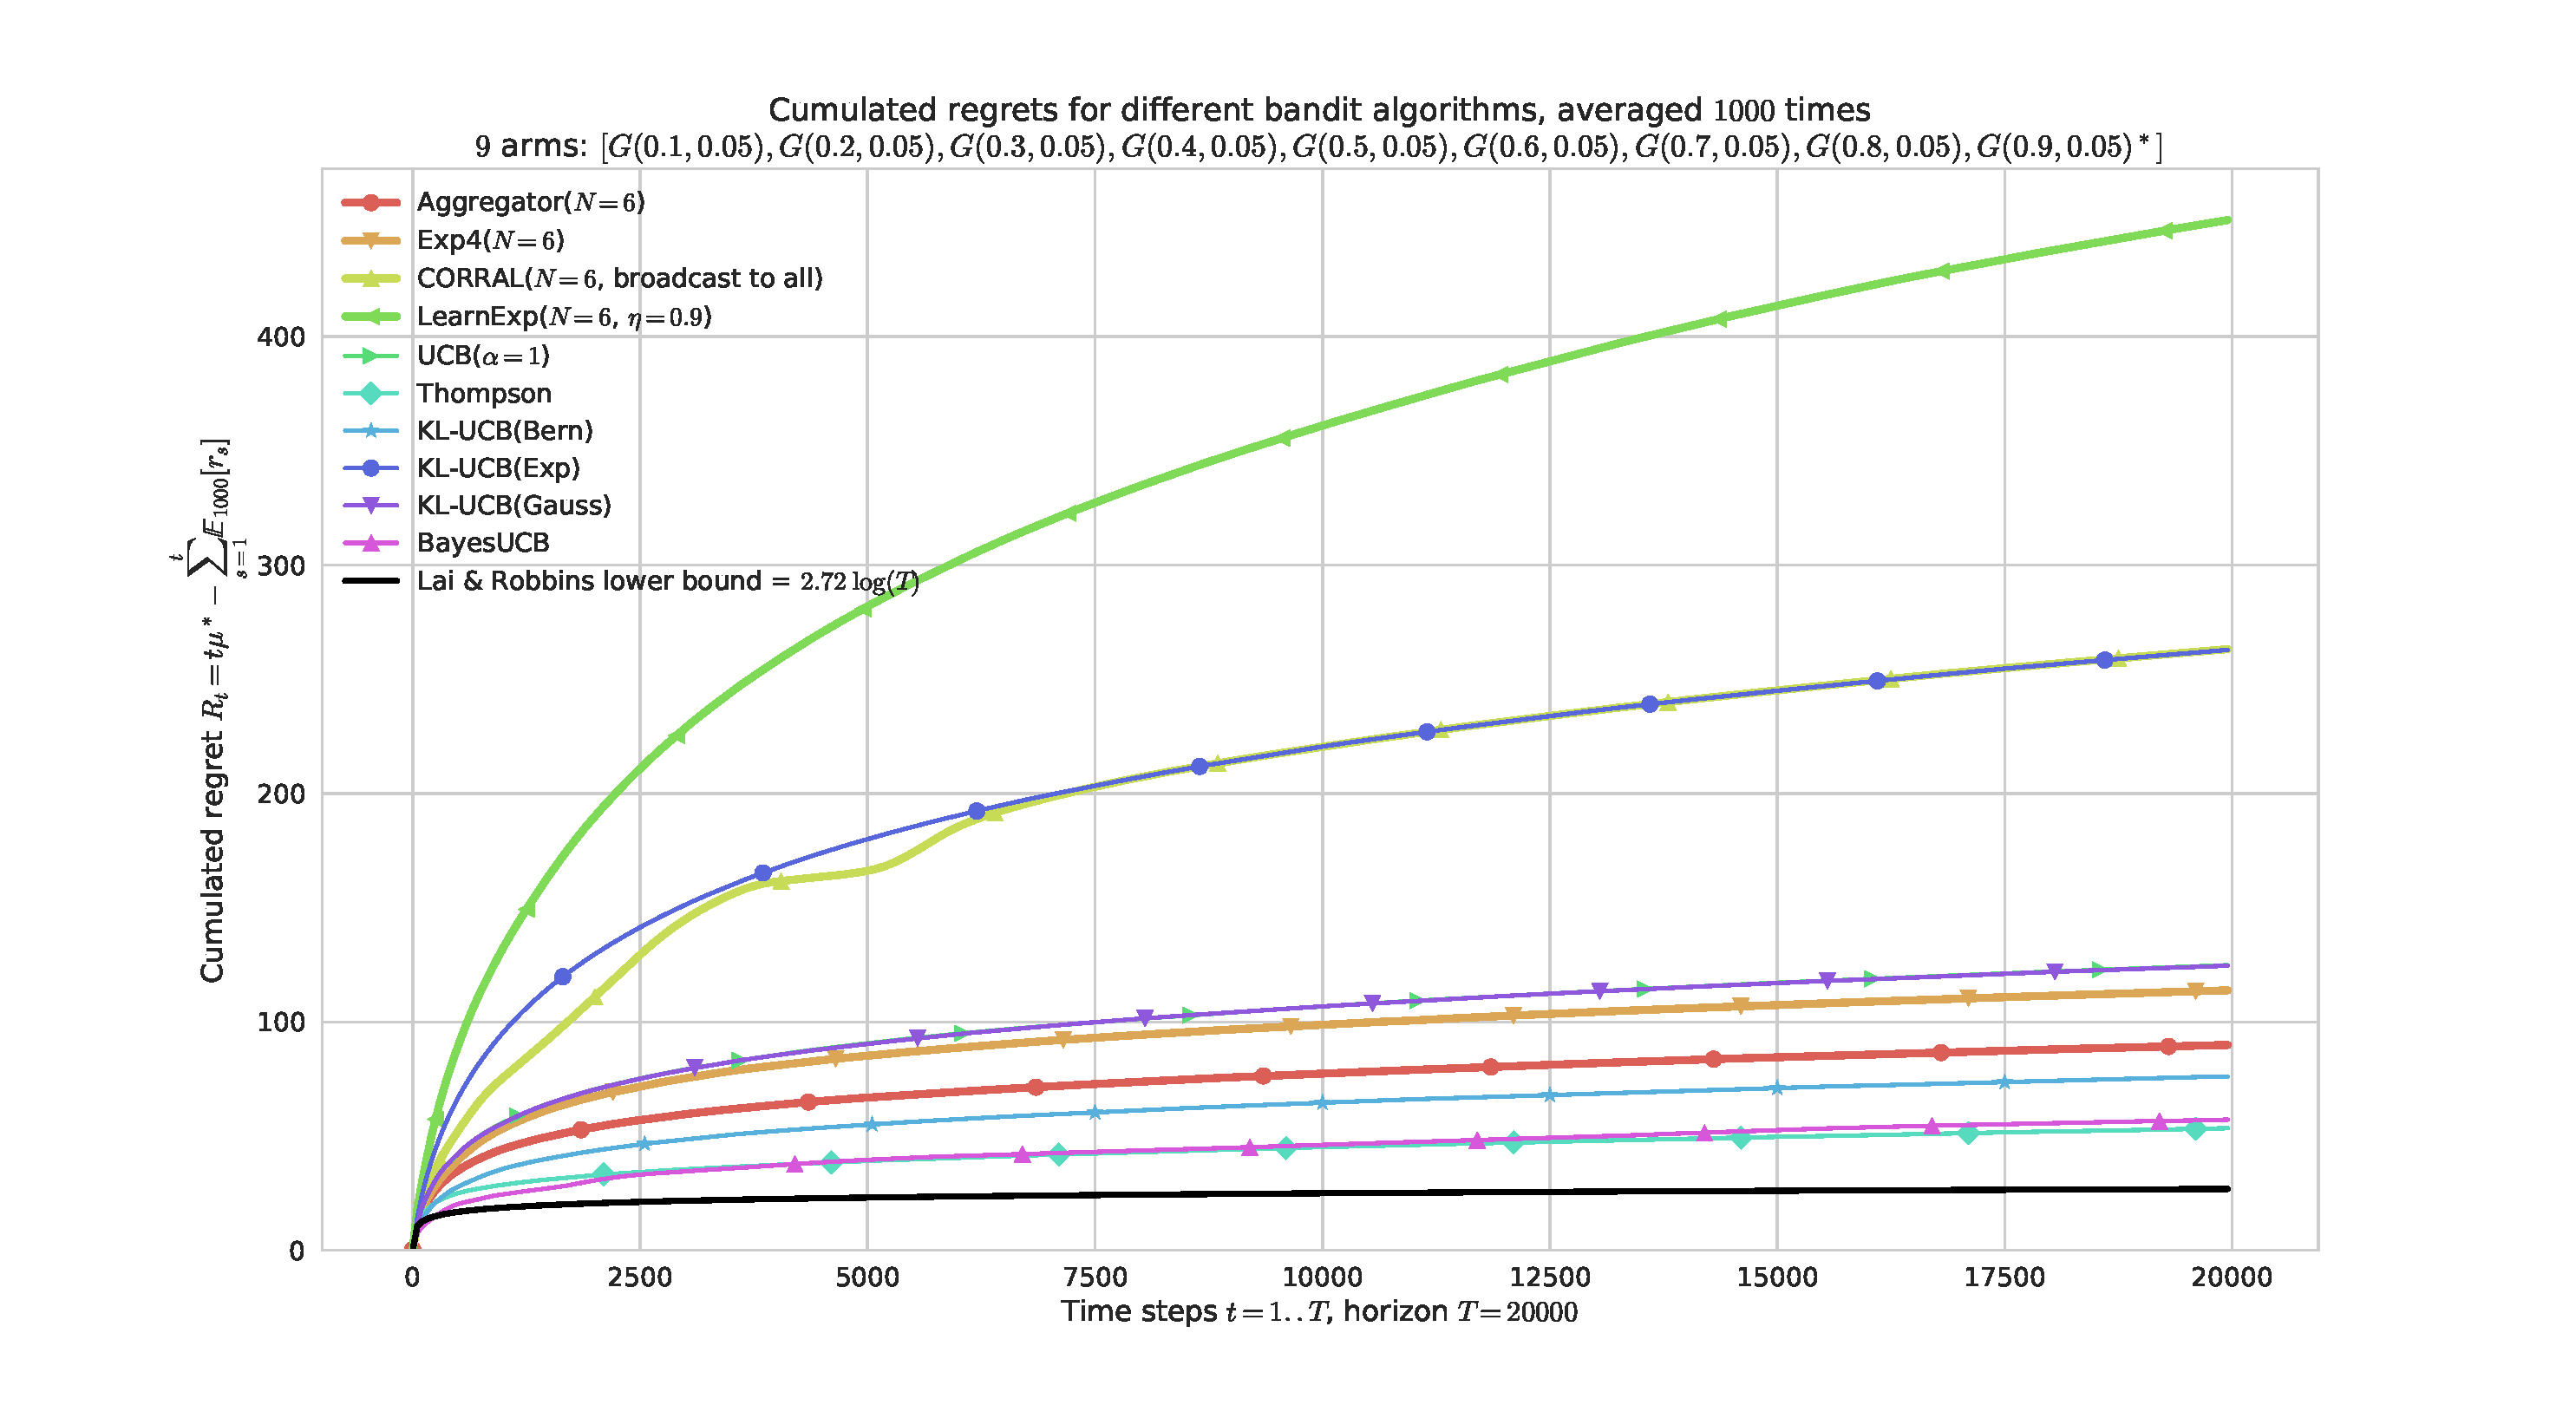
\includegraphics[width=1.10\linewidth]{2-Chapters/2-Chapter/IEEE_WCNC_2018.git/plots/main____env3-4_932221613383548446.pdf}
	\caption{On an ``easy'' Gaussian problem, only \Aggr{} shows reasonable performances, thanks to BayesUCB and Thompson sampling.}
	\label{fig:25:EasyGaussian}
\end{figure}

\begin{figure}[h!]  % [htbp]
	\centering
	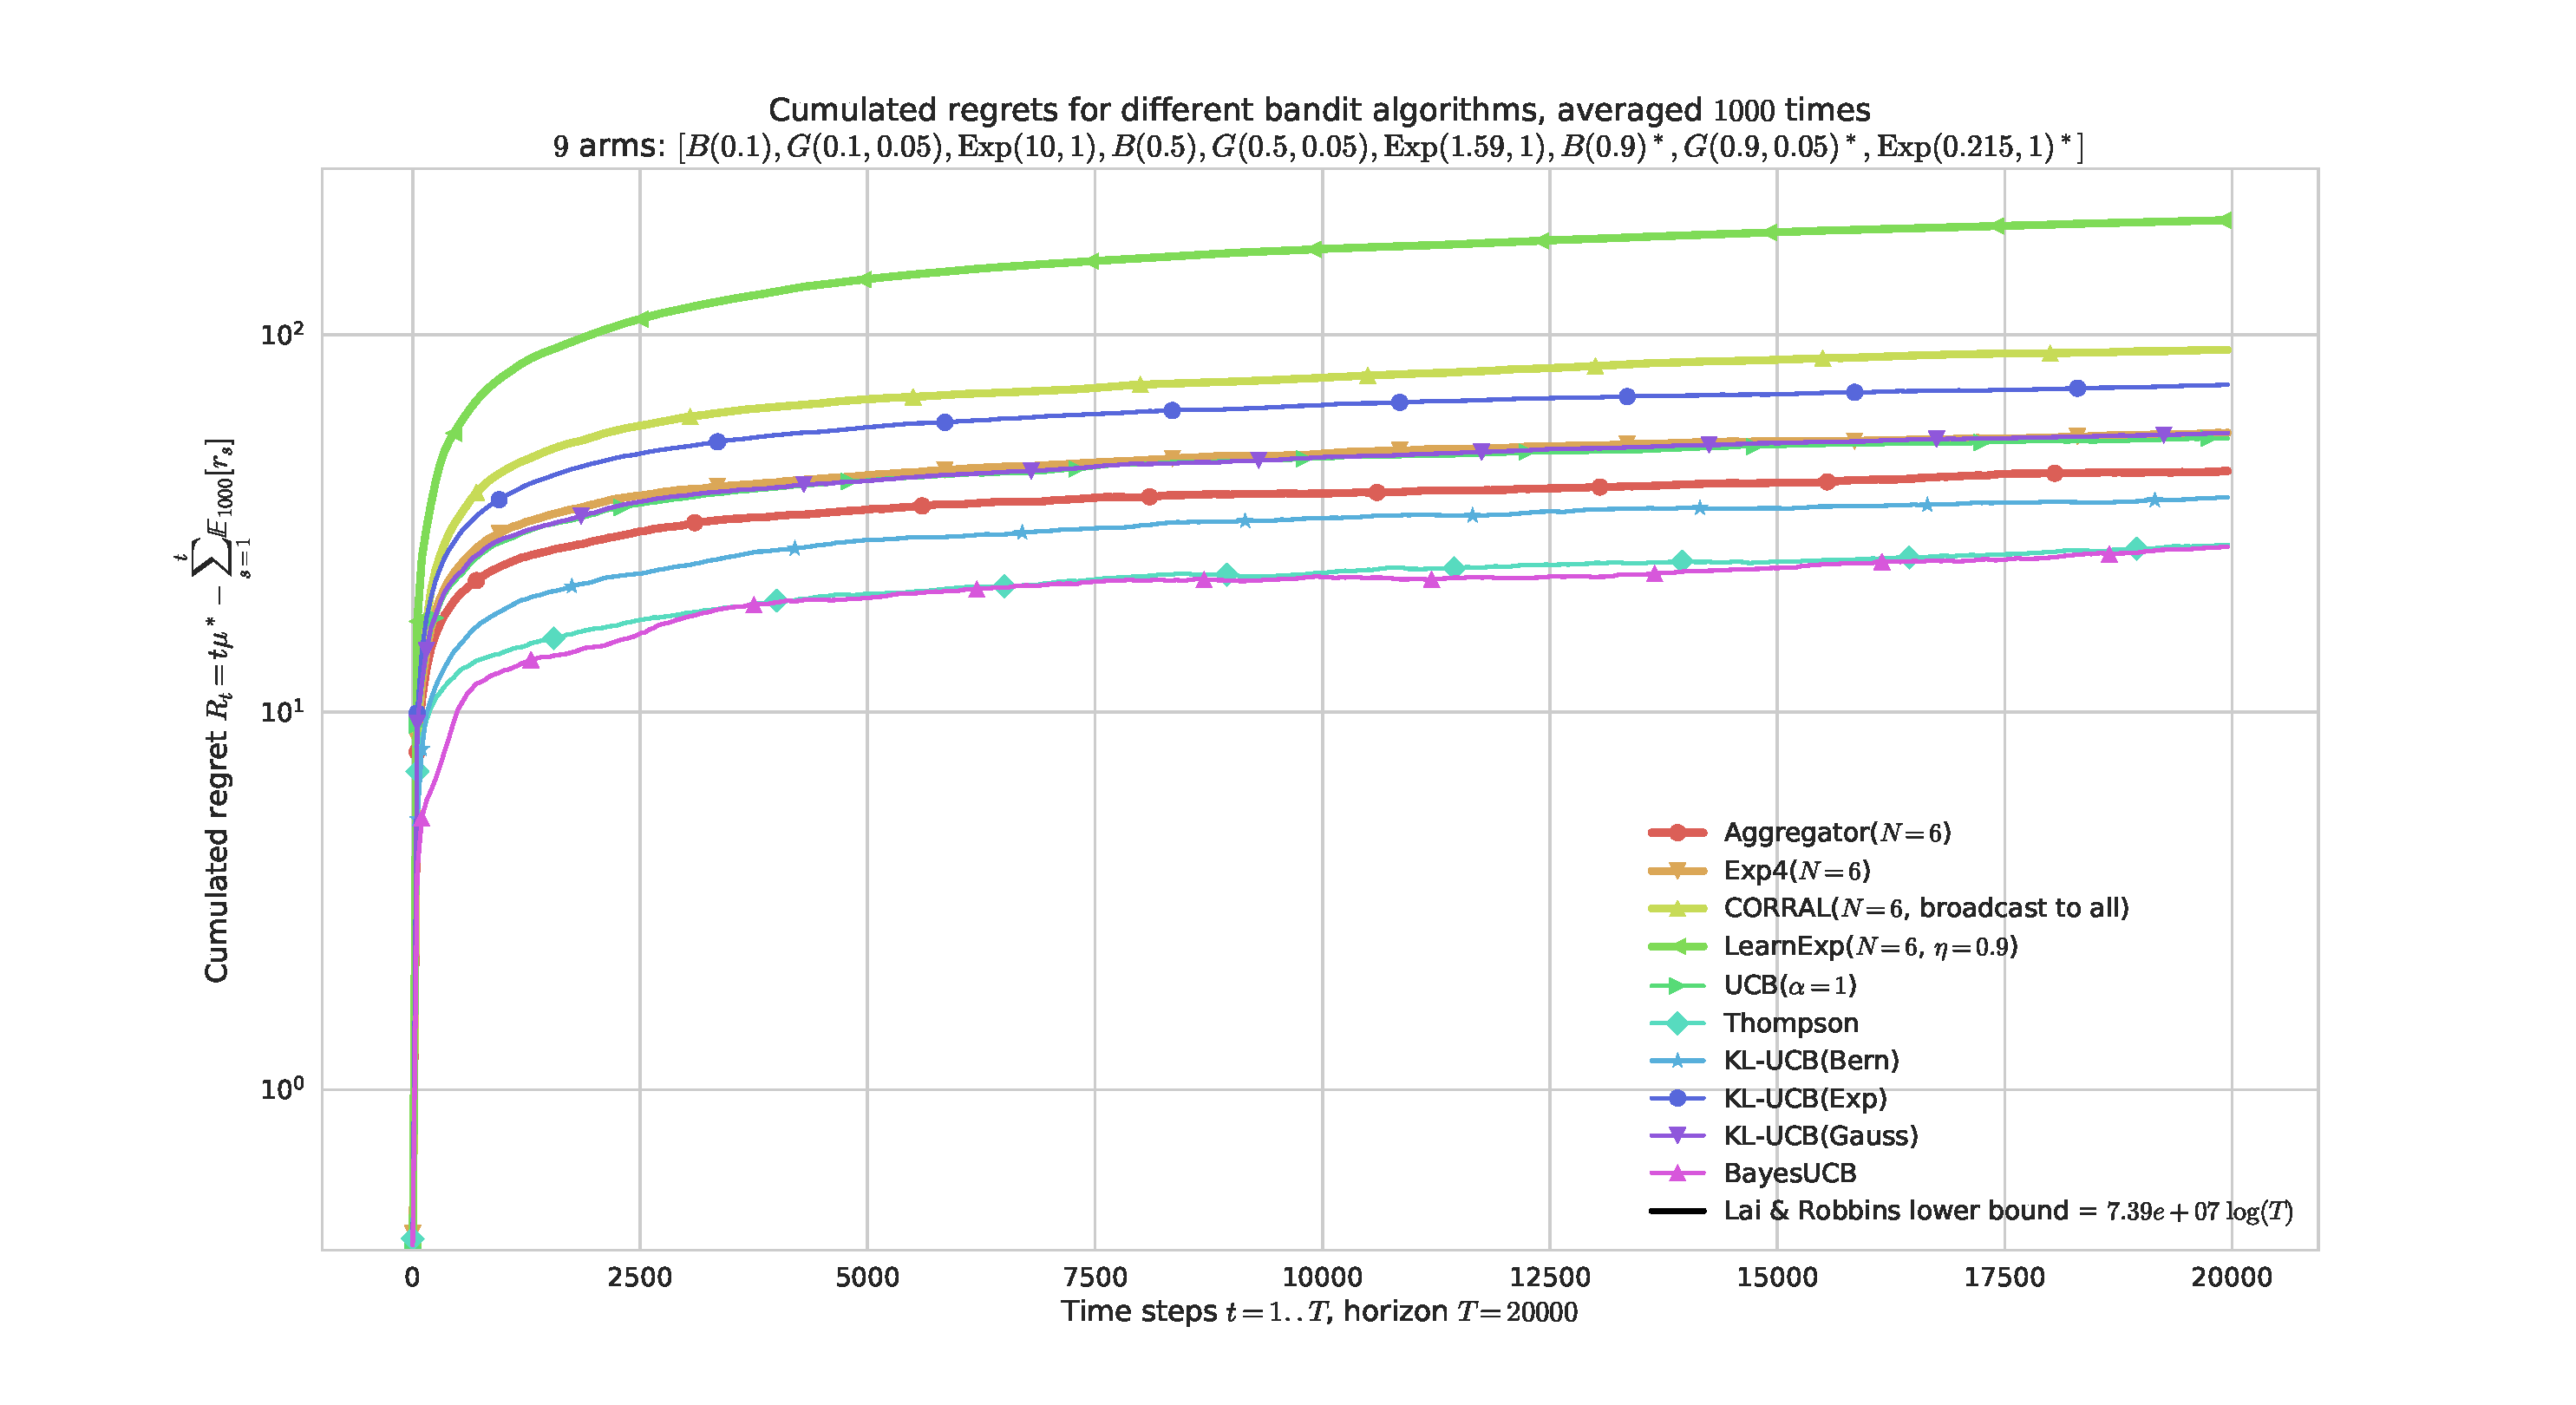
\includegraphics[width=1.10\linewidth]{2-Chapters/2-Chapter/IEEE_WCNC_2018.git/plots/main_semilogy____env4-4_932221613383548446.pdf}
	\caption{On a harder problem, mixing Bernoulli, Gaussian, Exponential arms, with 3 arms of each types with the \emph{same mean}.}
	\label{fig:25:HarderMixed}
\end{figure}

\begin{figure}[b!]  % [htbp]
	\centering
	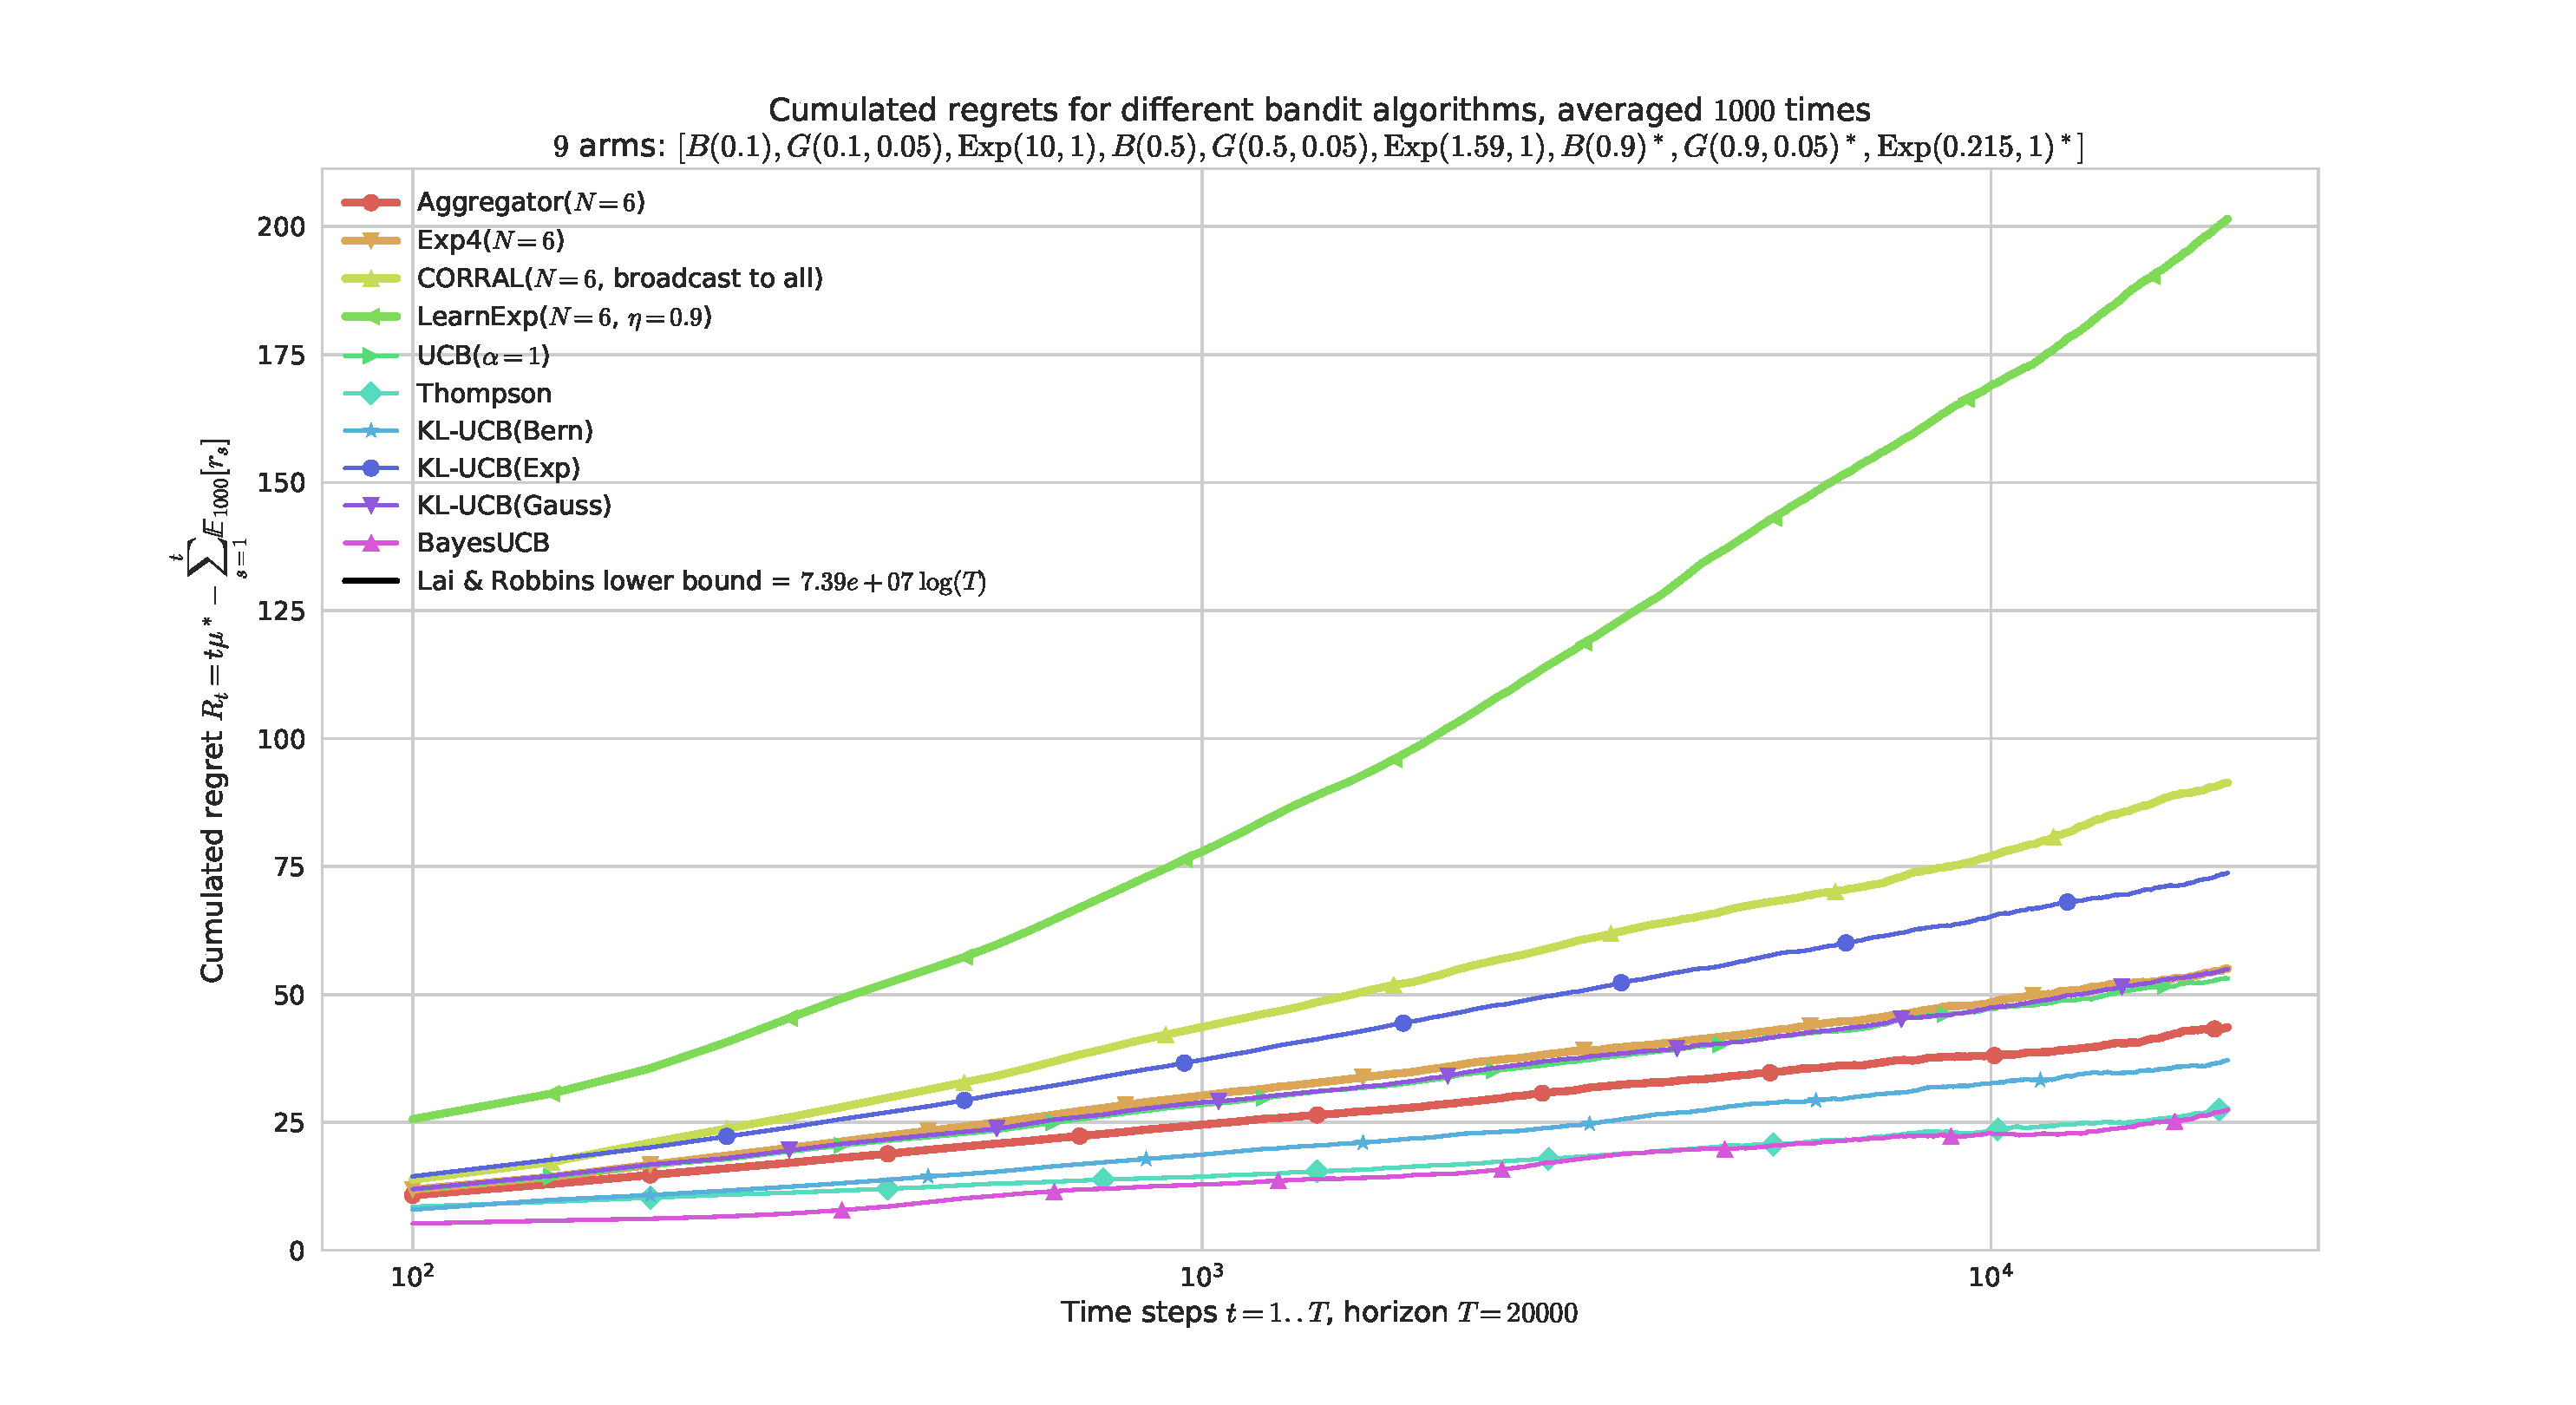
\includegraphics[width=1.10\linewidth]{2-Chapters/2-Chapter/IEEE_WCNC_2018.git/plots/main_semilogx____env4-4_932221613383548446.pdf}
	\caption{The semilog-$x$ scale clearly shows the logarithmic growth of the regret for the best algorithms and our proposal \Aggr, even in a hard ``mixed'' problem (\emph{cf}. Figure~\ref{fig:25:HarderMixed}).}
	\label{fig:25:HarderMixed_semilogx}
\end{figure}

For Bernoulli problems (Figures~\ref{fig:25:EasyBernoulli} and \ref{fig:25:HardBernoulli}), UCB with $\alpha=1/2$, Thompson sampling, BayesUCB and \klUCB{}$^+$ (with the binary $\kl$ function) all perform similarly, and \Aggr{} is found to be as efficient as all of them.
For Gaussian and exponential arms, rewards are truncated into $[0,1]$, and the variance of Gaussian distributions is fixed to $\sigma^2 = 0.05$ for all arms, and can be known to the algorithms (the \kl{} function is adapted to this one-dimensional exponential family).
%
Figure~\ref{fig:25:EasyGaussian} uses only Gaussian arms, with a large gap between their means and a relatively small variance, giving an ``easy'' problem.
%
And Figure~\ref{fig:25:HarderMixed} shows a considerably harder ``mixed'' problem, when the distributions are no longer in the same one-dimensional exponential family and so the Lai \& Robbins' lower-bound no longer holds (even if there still exists a lower-bound).

For each of the 4 problems considered, the \Aggr{} algorithm with default option (broadcast loss to all players) is the best of all the aggregation algorithms,
and its regret is very close to the best of the aggregated algorithms.
Especially in difficult problems with mixed or unknown distributions, \Aggr{} showed to be more efficient that \ExpQ{} and orders of magnitude better than the other reference aggregation algorithms \LearnExp{} and \CORRAL{} (see Figures~\ref{fig:25:HarderMixed} and \ref{fig:25:HarderMixed_semilogx}).


% ----------------------------------------------------------------------
\paragraph{No theoretical guarantees yet}\label{sub:25:theory}

The \Aggr{} does not have satisfying theoretical guarantees in terms of regret $R_T$, unlike many bandit algorithms.
%
Another notion, the \emph{adversarial regret}, denoted by $\overline{R_T}$,
measures the difference in terms of rewards,
between the aggregation algorithm $\Alg_{\mathrm{aggr}}$ and the best aggregated algorithm $\Alg_a$. This is in contrast with the (classical) regret, which measure the difference with the best fixed-arm strategy (Definition~\ref{def:2:regret}).
Thus, even if the aggregated algorithms have logarithmic (classical) regret, having an adversarial regret scaling as $\sqrt{T}$ does not permit to exhibit a logarithmic (classical) regret for the aggregation algorithm.
%
%
Under some additional hypotheses,
\cite[Theorem 4.2]{Bubeck12} proves that
\ExpQ{} satisfies a bound on adversarial regret, % $\overline{R_T}$
$\overline{R_T} \leq 2 \sqrt{T N \log(K)$,
with the good choice of the learning rate sequence $(\eta_t)_{t \geq 1}$.
Our proposed algorithm follows quite closely the architecture of \ExpQ,
and a similar bound for \Aggr{} is expected to hold.
% this is left as a future work.
% For sake of conciseness, we cannot present a proof here.
%

This would be a first theoretical guarantee, but not satisfactory as we saw above that simple algorithms (like \UCB) have regrets scaling as $\log(T)$ \cite{Auer02,Bubeck12}, not $\sqrt{T}$.
%
Regret bounds in several different settings are proved for the \CORRAL{} algorithm \cite{Agarwal16}, but no logarithmic upper-bound can be obtained from their technique, even in the simplest setting of stochastic bandits.
%
However, \Aggr{} always seems to have a (finite-horizon) logarithmic regret in all the experiments we performed,
for both Bernoulli and non-Bernoulli problems (\eg, Gaussian, exponential and Poisson distributions).
Further theoretical developments are left as future work.


% ----------------------------------------------------------------------
\paragraph{Conclusion about our \Aggr{} algorithm}\label{sub:25:conclusion}

We presented the use of aggregation algorithms in the context of Opportunistic Spectrum Access for Cognitive Radio,
especially for the real-world setting of unknown problem instances,
when tuning parameters before-hand is no longer possible and an adaptive algorithm is preferable.
% - \ExpQ and \Aggr works fine
% Both algorithms \ExpQ{} and \Aggr{} have been detailed, and we explained why
Our proposed \Aggr{} was presented in details,
and we also highlighted its differences with \ExpQ.
% as well \color{red} as the intuition that it seems more suited for purely stochastic problems\color{black}.

% - \Aggr{} really help to select the best algorithm against a certain problem, on the fly without any prior knowledge of the problem neither any prior knowledge on which algorithms is the best
We presented experiments on simple MAB problems coming from previous work on bandits for OSA \cite{Jouini10},
and the simulations results showed that \Aggr{} is able to identify on the fly the best algorithm to trust for a specific problem, as expected.
Experiments on problems mixing different families of distributions were also presented, with similar conclusions in favor of \Aggr.
It is not presented in this section, but our proposed algorithm also works well in dynamic scenarios, in which the distribution of the arms can change abruptly at some time,
and appears to be more robust than simple non-aggregated algorithms.

\ExpQ{} has theoretical guarantees in terms of adversarial regret, and even if the same result could hold for \Aggr, results in terms of classical regret are yet to be proved.
Empirically, \Aggr{} showed to always have a logarithmic
regret $R_T$ if it aggregates algorithms with logarithmic regrets (like UCB, \klUCB, Thompson sampling, BayesUCB etc).
It usually succeeds to be close to the best of the aggregated algorithms, both in term of regret and best arm pull frequency.
As expected, the \Aggr{} is never able to outperform any of the aggregated algorithms, but this was an over-optimistic goal.
%
What matters the most is that, empirically, \Aggr{} is able to quickly discover \emph{on the fly} the best algorithms to trust, and then performs almost as well as if it was following it from the beginning.

Our \Aggr{} algorithm could be rewritten as an Online Mirror Descent \cite{Hazan2016introduction,Zimmert2018}, as it is the case for both \ExpQ{} and \CORRAL.
But this direction does not appear very useful, as in the case of \CORRAL{}  the analysis cannot bring a logarithmic regret bound, even by aggregating asymptotically optimal algorithms.
% We will continue investigating regret bounds for \Aggr,
% and other directions include possible applications to the non-stochastic case (\eg, rested or restless Markovian problems, like it was very recently studied in \cite{Luo18}).

\paragraph{Reproducility of the experiments.}
%
Experiments presented in this Section are based on our library SMPyBandits,
and the page \texttt{SMPyBandits.GitHub.io/Aggregation.html} gives instructions to reproduce them.


% ----------------------------------------------------------------------------
% \bibliographystyle{ieeetr}
% \bibliography{IEEE_WCNC__2018__Paper__Lilian_Besson__07-17}


% A last solution is online algorithm selection, inspired from expert aggregation.
% Include here the discussion about expert aggregation and my \textbf{Aggregator} algorithm, see https://hal.inria.fr/hal-01705292


\newpage  % WARNING ?

% ----------------------------------------------------------------------------
\section{Conclusion}
\label{sec:2:conclusion}

In this chapter, we presented the multi-armed bandit model, focussing on a finite number of arms, and real-valued rewards.
Our main focus is on one-dimensional exponential families of distributions, and on stochastic and stationary problems.
By showcasing an interactive demonstration made available online,
% XXX ?
% (\href{https://perso.crans.org/besson/phd/MAB\_interactive\_demo/}{\texttt{perso.crans.org/besson/phd/MAB\_interactive\_demo/}}),
we presented the notations used in all this thesis.

The first contribution of this manuscript concludes this chapter, in Section~\ref{sec:2:chooseYourPreferredBanditAlgorithm}.
% and corresponds to our article \cite{Besson2018WCNC}.
We tackle the question of how to select a particular bandit algorithm when a practitioner is facing a particular (unknown) bandit problem.
Instead of always choosing a fixed algorithm, or running costly benchmarks before real-world deployment of the chosen algorithm, we advise to select a few candidate algorithms, where at least one is expected to be very efficient for the given problem, and use online algorithm selection to automatically and dynamically decide the best candidate.
We proposed an extension of the Exp4 algorithm for this problem, \Aggr, and illustrate its performance on some bandit problems.
%
The numerical simulations used our Python open-source library, SMPyBandits, that is presented in details in the next Chapter~\ref{chapter:3}.
The next chapter also includes simulations of the most important MAB algorithms that we presented above, on Bernoulli distributed problems of various sizes and durations.

We presented the simplest MAB model studied in this chapter, by focussing on one agent playing a stationary game.
Both hypotheses are removed or weaken in the rest of this manuscript,
% first in Chapter~\ref{chapter:4} where we consider many XXX
first by considering players facing a stationary problem in a decentralized way in Chapter~\ref{chapter:5},
and then by considering a single player facing a non-stationary or a piece-wise stationary problem in Chapter~\ref{chapter:6}.
%
For both directions, we present in the two final chapters natural extensions of the base model, and we detail our contributions that obtained state-of-the-art results for the two problems
of stationary multi-players and piece-wise stationary bandits.

We take another approach in Chapter~\ref{chapter:4}, where the MAB model is generalized to study decentralized learning of a large set of independent players, all having different activation times.
This extension is significantly harder than the two previously evoked ones, and we were unfortunately unable to obtain any strong theoretical results under these loose hypotheses.
This model is however more generic and as such it was found suitable for applications to Internet of Things (IoT) networks, where arms model orthogonal wireless channels, players model communicating devices (\ie, IoT end-devices) and rewards model successes or failures of a wireless packet sent by a device.


\paragraph{Possible future works.}
%
We focused in this thesis on finite-arms and one-dimensional bandit problems,
and thus two possible directions of future works could be to extend our works
to MAB models with either multidimensional rewards, like contextual bandits, or infinite arms, like Lipschitz bandits.


% % % ----------------------------------------------------------------------------
% \section{Appendix}
% \label{sec:2:appendix}


% % ----------------------------------------------------------------------------
% \subsubsection{Pinsker's inequality}\label{proof:2:Pinsker}

% We prove it below using simple real analysis arguments,
% % \footnote{~The proof is inspired by Lemma~10.2 from \cite{LattimoreBanditAlgorithmsBook} (version $1699$ of January $2019$).},
% %
% and for instance we use it again in Chapter~\ref{chapter:6}.
% %
% Moreover, using the notations of the exponential families for Bernoulli and fixed-variance Gaussian distributions (see above Section~\ref{par:2:notationsExponentialFamiliesBernoulliGaussian}), it can be written $\kl(x,y) \geq d_{1/4}(x,y)$.
% %
% As bounded distributions in $[0,1]$ are sub-Bernoulli as well as $1/4$-sub-Gaussian, one consequence of this inequality is that the confidence radius of \klUCB{} is \emph{smaller} than the one in $\UCB_1$, and different concentration inequalities can then be used to prove their finite-time logarithmic regret upper-bounds, and to prove that \klUCB{} is asymptotically optimal while $\UCB_1$ is only order-optimal for bounded rewards (see above in Section~\ref{proof:2:UCBregretBound} or \cite{Auer02} for $\UCB_1$, and \cite{KLUCBJournal} for \klUCB).


% \begin{lemma}[Pinsker's inequality]\label{lem:2:Pinsker}
% \begin{leftbar}[lemmabar]  % XXX leftbar lemmabar, comment if needed
%     Let $p,q\in[0,1]$, and remember that the \emph{relative binary entropy} is defined as $\kl(p,q) \eqdef p \ln\left(\frac{p}{q}\right) + (1-p)\ln\left(\frac{1-p}{1-q}\right)$.

%     Then for any $p,q\in[0,1]$, $\kl$ verifies $\kl(p,q) \geq 2 (p-q)^2$.
% \end{leftbar}  % XXX leftbar lemmabar, comment if needed
% \end{lemma}

% \begin{smallproof}
%     Fix $p\in[0,1]$, and consider the function $g(x) \eqdef \kl(p, p+x) - 2 x^2$ ($x$ will be $q-p$), for $x\in(-p, 1-p)$.
%     We first observe that $g(0) = 0$, and we easily prove that $x=0$ is the unique minimizer of $g$ over its domain.
%     By definition, $\kl$ is of class $\cC^1$ on its two variables, on the open interval $(0,1)$, so $g$ is of class $\cC^1$ on the interior of its domain, $(-p, 1-p)$.
%     Let us compute its derivative, $g'(x) = (\frac{\partial \; \kl}{\partial 2})(p, p + x) - 4x$.
%     Simple calculus yield
%     \[ \left(\frac{\partial \; \kl}{\partial 2}\right) (p, p + x) = - \frac{p}{p+x} + \frac{1-p}{1-(p+x)} = -x \frac{(2(p + x) - 1)^2}{(p + x)(p + x - 1)}. \]
%     % https://www.wolframalpha.com/input/?i=diff(p+*+log(p%2F(p%2Bx))+%2B+(1-p)+*+log((1-p)%2F(1-(p%2Bx)))+-+2*x**2,+x)
%     We can verify that $g'(0) = -1 + 1 - 4 \times 0 = 0$, and it has the sign of $-x$ on its domain, as $p + x - 1 < 0$ because $x < 1 - p$, and $p + x > 0$.
%     So $g'$ is first positive then negative, so $g$ is increasing then decreasing on its domain, with a change in its monotony at $x=0$, and thus it indeed has a unique minimizer.
%     We conclude that $g(x) \geq g(0) = 0$ on $(-p, 1-p)$, and so $\kl(p,q) \geq 2 (p-q)^2$ if $x = q-p$.

%     The edge case is the ends of the interval, that is if $x=-p$ or $x=1-p$, that is if $q=0$ or $q=1$.
%     If $p\in(0,1)$, then computing the limit of $\kl(p,q)$ for $q\to0^+$ and $q\to1^-$ is obvious and gives $\kl(p,q) \to +\infty$, while the right-hand side of Pinsker's inequality stays finite (so the inequality is still true at the limit).
%     If $p=0$ or $p=1$, the same computation works, by the convention that $p \log(p) = 0$ if $p=0$.
%     %
%     % Bonus: one can verify our computation in Python with the SymPy module:
%     % \begin{verbatim}
%     %     $ (bash) python
%     %     >>> from sympy import *
%     %     >>> x, p = symbols('x p')
%     %     >>> g = p * log(p/(p+x)) + (1-p) * log((1-p)/(1-(p+x))) - 2*x**2
%     %     >>> print(diff(g, x))
%     %     -p/(p + x) - 4*x + (-p + 1)/(-p - x + 1)
%     % \end{verbatim}
% \end{smallproof}
